\documentclass[twoside]{book}

% Packages required by doxygen
\usepackage{fixltx2e}
\usepackage{calc}
\usepackage{doxygen}
\usepackage[export]{adjustbox} % also loads graphicx
\usepackage{graphicx}
\usepackage[utf8]{inputenc}
\usepackage{makeidx}
\usepackage{multicol}
\usepackage{multirow}
\PassOptionsToPackage{warn}{textcomp}
\usepackage{textcomp}
\usepackage[nointegrals]{wasysym}
\usepackage[table]{xcolor}

% Font selection
\usepackage[T1]{fontenc}
\usepackage[scaled=.90]{helvet}
\usepackage{courier}
\usepackage{amssymb}
\usepackage{sectsty}
\renewcommand{\familydefault}{\sfdefault}
\allsectionsfont{%
  \fontseries{bc}\selectfont%
  \color{darkgray}%
}
\renewcommand{\DoxyLabelFont}{%
  \fontseries{bc}\selectfont%
  \color{darkgray}%
}
\newcommand{\+}{\discretionary{\mbox{\scriptsize$\hookleftarrow$}}{}{}}

% Page & text layout
\usepackage{geometry}
\geometry{%
  a4paper,%
  top=2.5cm,%
  bottom=2.5cm,%
  left=2.5cm,%
  right=2.5cm%
}
\tolerance=750
\hfuzz=15pt
\hbadness=750
\setlength{\emergencystretch}{15pt}
\setlength{\parindent}{0cm}
\setlength{\parskip}{0.2cm}
\makeatletter
\renewcommand{\paragraph}{%
  \@startsection{paragraph}{4}{0ex}{-1.0ex}{1.0ex}{%
    \normalfont\normalsize\bfseries\SS@parafont%
  }%
}
\renewcommand{\subparagraph}{%
  \@startsection{subparagraph}{5}{0ex}{-1.0ex}{1.0ex}{%
    \normalfont\normalsize\bfseries\SS@subparafont%
  }%
}
\makeatother

% Headers & footers
\usepackage{fancyhdr}
\pagestyle{fancyplain}
\fancyhead[LE]{\fancyplain{}{\bfseries\thepage}}
\fancyhead[CE]{\fancyplain{}{}}
\fancyhead[RE]{\fancyplain{}{\bfseries\leftmark}}
\fancyhead[LO]{\fancyplain{}{\bfseries\rightmark}}
\fancyhead[CO]{\fancyplain{}{}}
\fancyhead[RO]{\fancyplain{}{\bfseries\thepage}}
\fancyfoot[LE]{\fancyplain{}{}}
\fancyfoot[CE]{\fancyplain{}{}}
\fancyfoot[RE]{\fancyplain{}{\bfseries\scriptsize Generated on Mon Nov 16 2015 23\+:21\+:16 for Item\+Prototype by Doxygen }}
\fancyfoot[LO]{\fancyplain{}{\bfseries\scriptsize Generated on Mon Nov 16 2015 23\+:21\+:16 for Item\+Prototype by Doxygen }}
\fancyfoot[CO]{\fancyplain{}{}}
\fancyfoot[RO]{\fancyplain{}{}}
\renewcommand{\footrulewidth}{0.4pt}
\renewcommand{\chaptermark}[1]{%
  \markboth{#1}{}%
}
\renewcommand{\sectionmark}[1]{%
  \markright{\thesection\ #1}%
}

% Indices & bibliography
\usepackage{natbib}
\usepackage[titles]{tocloft}
\setcounter{tocdepth}{3}
\setcounter{secnumdepth}{5}
\makeindex

% Hyperlinks (required, but should be loaded last)
\usepackage{ifpdf}
\ifpdf
  \usepackage[pdftex,pagebackref=true]{hyperref}
\else
  \usepackage[ps2pdf,pagebackref=true]{hyperref}
\fi
\hypersetup{%
  colorlinks=true,%
  linkcolor=blue,%
  citecolor=blue,%
  unicode%
}

% Custom commands
\newcommand{\clearemptydoublepage}{%
  \newpage{\pagestyle{empty}\cleardoublepage}%
}


%===== C O N T E N T S =====

\begin{document}

% Titlepage & ToC
\hypersetup{pageanchor=false,
             bookmarks=true,
             bookmarksnumbered=true,
             pdfencoding=unicode
            }
\pagenumbering{roman}
\begin{titlepage}
\vspace*{7cm}
\begin{center}%
{\Large Item\+Prototype }\\
\vspace*{1cm}
{\large Generated by Doxygen 1.8.10}\\
\vspace*{0.5cm}
{\small Mon Nov 16 2015 23:21:16}\\
\end{center}
\end{titlepage}
\clearemptydoublepage
\tableofcontents
\clearemptydoublepage
\pagenumbering{arabic}
\hypersetup{pageanchor=true}

%--- Begin generated contents ---
\chapter{Deprecated List}
\label{deprecated}
\hypertarget{deprecated}{}

\begin{DoxyRefList}
\item[\label{deprecated__deprecated000008}%
\hypertarget{deprecated__deprecated000008}{}%
Class \hyperlink{class_json_1_1_fast_writer}{Json\+:\+:Fast\+Writer} ]Use \hyperlink{class_json_1_1_stream_writer_builder}{Stream\+Writer\+Builder}.  
\item[\label{deprecated__deprecated000005}%
\hypertarget{deprecated__deprecated000005}{}%
Class \hyperlink{class_json_1_1_reader}{Json\+:\+:Reader} ]Use \hyperlink{class_json_1_1_char_reader}{Char\+Reader} and \hyperlink{class_json_1_1_char_reader_builder}{Char\+Reader\+Builder}.  
\item[\label{deprecated__deprecated000006}%
\hypertarget{deprecated__deprecated000006}{}%
Member \hyperlink{class_json_1_1_reader_afa4a59e962d23c4d1c38b433fc95eefa}{Json\+:\+:Reader\+:\+:get\+Formated\+Error\+Messages} () const ]Use \hyperlink{class_json_1_1_reader_a95ab50aa789132e9dee0fc1475c85acf}{get\+Formatted\+Error\+Messages()} instead (typo fix).  
\item[\label{deprecated__deprecated000010}%
\hypertarget{deprecated__deprecated000010}{}%
Class \hyperlink{class_json_1_1_styled_stream_writer}{Json\+:\+:Styled\+Stream\+Writer} ]Use \hyperlink{class_json_1_1_stream_writer_builder}{Stream\+Writer\+Builder}.  
\item[\label{deprecated__deprecated000009}%
\hypertarget{deprecated__deprecated000009}{}%
Class \hyperlink{class_json_1_1_styled_writer}{Json\+:\+:Styled\+Writer} ]Use \hyperlink{class_json_1_1_stream_writer_builder}{Stream\+Writer\+Builder}.  
\item[\label{deprecated__deprecated000002}%
\hypertarget{deprecated__deprecated000002}{}%
Member \hyperlink{class_json_1_1_value_ae1f95f7ca3906e6bcc2a7be93210ecba}{Json\+:\+:Value\+:\+:remove\+Member} (const std\+::string \&key)]
\item[\label{deprecated__deprecated000001}%
\hypertarget{deprecated__deprecated000001}{}%
Member \hyperlink{class_json_1_1_value_aa52f7873b95d29627d6e83ba96f69aaa}{Json\+:\+:Value\+:\+:remove\+Member} (const char $\ast$key)]
\item[\label{deprecated__deprecated000003}%
\hypertarget{deprecated__deprecated000003}{}%
Member \hyperlink{class_json_1_1_value_a29f3a30f7e5d3af6f38d57999bf5b480}{Json\+:\+:Value\+:\+:set\+Comment} (const char $\ast$comment, Comment\+Placement placement)]Always pass len.  
\item[\label{deprecated__deprecated000004}%
\hypertarget{deprecated__deprecated000004}{}%
Member \hyperlink{class_json_1_1_value_iterator_base_ac3aa3870761342e47c6486d81f643c6c}{Json\+:\+:Value\+Iterator\+Base\+:\+:member\+Name} () const ]This cannot be used for U\+T\+F-\/8 strings, since there can be embedded nulls.  
\item[\label{deprecated__deprecated000007}%
\hypertarget{deprecated__deprecated000007}{}%
Class \hyperlink{class_json_1_1_writer}{Json\+:\+:Writer} ]Use \hyperlink{class_json_1_1_stream_writer}{Stream\+Writer}. (And really, this is an implementation detail.) 
\end{DoxyRefList}
\chapter{Namespace Index}
\section{Namespace List}
Here is a list of all documented namespaces with brief descriptions\+:\begin{DoxyCompactList}
\item\contentsline{section}{\hyperlink{namespace_json}{Json} \\*J\+S\+O\+N (Java\+Script Object Notation) }{\pageref{namespace_json}}{}
\end{DoxyCompactList}

\chapter{Hierarchical Index}
\section{Class Hierarchy}
This inheritance list is sorted roughly, but not completely, alphabetically\+:\begin{DoxyCompactList}
\item \contentsline{section}{Item}{\pageref{class_item}}{}
\begin{DoxyCompactList}
\item \contentsline{section}{Antidote}{\pageref{class_antidote}}{}
\item \contentsline{section}{Potion}{\pageref{class_potion}}{}
\end{DoxyCompactList}
\item \contentsline{section}{Item\+Factory}{\pageref{class_item_factory}}{}
\end{DoxyCompactList}

\chapter{Class Index}
\section{Class List}
Here are the classes, structs, unions and interfaces with brief descriptions\+:\begin{DoxyCompactList}
\item\contentsline{section}{\hyperlink{class_antidote}{Antidote} \\*An \hyperlink{class_antidote}{Antidote} class }{\pageref{class_antidote}}{}
\item\contentsline{section}{\hyperlink{class_item}{Item} \\*Abstract \hyperlink{class_item}{Item} Class }{\pageref{class_item}}{}
\item\contentsline{section}{\hyperlink{class_item_factory}{Item\+Factory} \\*An \hyperlink{class_item_factory}{Item\+Factory} class }{\pageref{class_item_factory}}{}
\item\contentsline{section}{\hyperlink{class_potion}{Potion} \\*A \hyperlink{class_potion}{Potion} class inherited from \hyperlink{class_item}{Item} class }{\pageref{class_potion}}{}
\end{DoxyCompactList}

\chapter{Namespace Documentation}
\hypertarget{namespace_json}{}\section{Json Namespace Reference}
\label{namespace_json}\index{Json@{Json}}


J\+S\+O\+N (Java\+Script Object Notation).  


\subsection*{Classes}
\begin{DoxyCompactItemize}
\item 
struct \hyperlink{struct_json_1_1_built_styled_stream_writer}{Built\+Styled\+Stream\+Writer}
\item 
class \hyperlink{class_json_1_1_char_reader}{Char\+Reader}
\item 
class \hyperlink{class_json_1_1_char_reader_builder}{Char\+Reader\+Builder}
\begin{DoxyCompactList}\small\item\em Build a \hyperlink{class_json_1_1_char_reader}{Char\+Reader} implementation. \end{DoxyCompactList}\item 
struct \hyperlink{struct_json_1_1_comment_style}{Comment\+Style}
\begin{DoxyCompactList}\small\item\em Scoped enums are not available until C++11. \end{DoxyCompactList}\item 
class \hyperlink{class_json_1_1_exception}{Exception}
\item 
class \hyperlink{class_json_1_1_fast_writer}{Fast\+Writer}
\begin{DoxyCompactList}\small\item\em Outputs a \hyperlink{class_json_1_1_value}{Value} in \href{http://www.json.org}{\tt J\+S\+O\+N} format without formatting (not human friendly). \end{DoxyCompactList}\item 
class \hyperlink{class_json_1_1_features}{Features}
\begin{DoxyCompactList}\small\item\em Configuration passed to reader and writer. This configuration object can be used to force the \hyperlink{class_json_1_1_reader}{Reader} or \hyperlink{class_json_1_1_writer}{Writer} to behave in a standard conforming way. \end{DoxyCompactList}\item 
class \hyperlink{class_json_1_1_logic_error}{Logic\+Error}
\item 
class \hyperlink{class_json_1_1_our_char_reader}{Our\+Char\+Reader}
\item 
class \hyperlink{class_json_1_1_our_features}{Our\+Features}
\item 
class \hyperlink{class_json_1_1_our_reader}{Our\+Reader}
\item 
class \hyperlink{class_json_1_1_path}{Path}
\begin{DoxyCompactList}\small\item\em Experimental and untested\+: represents a \char`\"{}path\char`\"{} to access a node. \end{DoxyCompactList}\item 
class \hyperlink{class_json_1_1_path_argument}{Path\+Argument}
\begin{DoxyCompactList}\small\item\em Experimental and untested\+: represents an element of the \char`\"{}path\char`\"{} to access a node. \end{DoxyCompactList}\item 
class \hyperlink{class_json_1_1_reader}{Reader}
\begin{DoxyCompactList}\small\item\em Unserialize a \href{http://www.json.org}{\tt J\+S\+O\+N} document into a \hyperlink{class_json_1_1_value}{Value}. \end{DoxyCompactList}\item 
class \hyperlink{class_json_1_1_runtime_error}{Runtime\+Error}
\item 
class \hyperlink{class_json_1_1_static_string}{Static\+String}
\begin{DoxyCompactList}\small\item\em Lightweight wrapper to tag static string. \end{DoxyCompactList}\item 
class \hyperlink{class_json_1_1_stream_writer}{Stream\+Writer}
\item 
class \hyperlink{class_json_1_1_stream_writer_builder}{Stream\+Writer\+Builder}
\begin{DoxyCompactList}\small\item\em Build a \hyperlink{class_json_1_1_stream_writer}{Stream\+Writer} implementation. \end{DoxyCompactList}\item 
class \hyperlink{class_json_1_1_styled_stream_writer}{Styled\+Stream\+Writer}
\begin{DoxyCompactList}\small\item\em Writes a \hyperlink{class_json_1_1_value}{Value} in \href{http://www.json.org}{\tt J\+S\+O\+N} format in a human friendly way, to a stream rather than to a string. \end{DoxyCompactList}\item 
class \hyperlink{class_json_1_1_styled_writer}{Styled\+Writer}
\begin{DoxyCompactList}\small\item\em Writes a \hyperlink{class_json_1_1_value}{Value} in \href{http://www.json.org}{\tt J\+S\+O\+N} format in a human friendly way. \end{DoxyCompactList}\item 
class \hyperlink{class_json_1_1_value}{Value}
\begin{DoxyCompactList}\small\item\em Represents a \href{http://www.json.org}{\tt J\+S\+O\+N} value. \end{DoxyCompactList}\item 
class \hyperlink{class_json_1_1_value_const_iterator}{Value\+Const\+Iterator}
\begin{DoxyCompactList}\small\item\em const iterator for object and array value. \end{DoxyCompactList}\item 
class \hyperlink{class_json_1_1_value_iterator}{Value\+Iterator}
\begin{DoxyCompactList}\small\item\em Iterator for object and array value. \end{DoxyCompactList}\item 
class \hyperlink{class_json_1_1_value_iterator_base}{Value\+Iterator\+Base}
\begin{DoxyCompactList}\small\item\em base class for \hyperlink{class_json_1_1_value}{Value} iterators. \end{DoxyCompactList}\item 
class \hyperlink{class_json_1_1_writer}{Writer}
\begin{DoxyCompactList}\small\item\em Abstract class for writers. \end{DoxyCompactList}\end{DoxyCompactItemize}
\subsection*{Typedefs}
\begin{DoxyCompactItemize}
\item 
\hypertarget{namespace_json_a08122e8005b706d982e48cca1e2119c7}{}typedef int {\bfseries Int}\label{namespace_json_a08122e8005b706d982e48cca1e2119c7}

\item 
\hypertarget{namespace_json_a800fb90eb6ee8d5d62b600c06f87f7d4}{}typedef unsigned int {\bfseries U\+Int}\label{namespace_json_a800fb90eb6ee8d5d62b600c06f87f7d4}

\item 
\hypertarget{namespace_json_ab7b47d2905da3b4ae60e4e800ec9ae5f}{}typedef long long int {\bfseries Int64}\label{namespace_json_ab7b47d2905da3b4ae60e4e800ec9ae5f}

\item 
\hypertarget{namespace_json_a01f20bce8f8229f38ff890168c0e6452}{}typedef unsigned long long int {\bfseries U\+Int64}\label{namespace_json_a01f20bce8f8229f38ff890168c0e6452}

\item 
\hypertarget{namespace_json_a218d880af853ce786cd985e82571d297}{}typedef Int64 {\bfseries Largest\+Int}\label{namespace_json_a218d880af853ce786cd985e82571d297}

\item 
\hypertarget{namespace_json_ae202ecad69725e23443f465e257456d0}{}typedef U\+Int64 {\bfseries Largest\+U\+Int}\label{namespace_json_ae202ecad69725e23443f465e257456d0}

\item 
\hypertarget{namespace_json_a8048e741f2177c3b5d9ede4a5b8c53c2}{}typedef unsigned int {\bfseries Array\+Index}\label{namespace_json_a8048e741f2177c3b5d9ede4a5b8c53c2}

\item 
\hypertarget{namespace_json_a602bcf69c2042fb61c3b243cb16f04ca}{}typedef char {\bfseries U\+Int\+To\+String\+Buffer}\mbox{[}\hyperlink{namespace_json_a2aacab54ef6fc18e833fbd4982a0a23aae4f2008c7919f20d81286121d1374424}{uint\+To\+String\+Buffer\+Size}\mbox{]}\label{namespace_json_a602bcf69c2042fb61c3b243cb16f04ca}

\item 
\hypertarget{namespace_json_a4724efb8d41614b47036cb8b54233837}{}typedef std\+::auto\+\_\+ptr$<$ \hyperlink{class_json_1_1_char_reader}{Char\+Reader} $>$ {\bfseries Char\+Reader\+Ptr}\label{namespace_json_a4724efb8d41614b47036cb8b54233837}

\item 
\hypertarget{namespace_json_a7132404aeebfc96d7c6ad2c66260afb5}{}typedef std\+::auto\+\_\+ptr$<$ \hyperlink{class_json_1_1_stream_writer}{Stream\+Writer} $>$ {\bfseries Stream\+Writer\+Ptr}\label{namespace_json_a7132404aeebfc96d7c6ad2c66260afb5}

\end{DoxyCompactItemize}
\subsection*{Enumerations}
\begin{DoxyCompactItemize}
\item 
enum \hyperlink{namespace_json_a7d654b75c16a57007925868e38212b4e}{Value\+Type} \{ \\*
\hyperlink{namespace_json_a7d654b75c16a57007925868e38212b4ea7d9899633b4409bd3fc107e6737f8391}{null\+Value} = 0, 
\hyperlink{namespace_json_a7d654b75c16a57007925868e38212b4eae5a9d708d5c9e23ae9bf98898522512d}{int\+Value}, 
\hyperlink{namespace_json_a7d654b75c16a57007925868e38212b4eaea788d9a3bb00adc6d68d97d43e1ccd3}{uint\+Value}, 
\hyperlink{namespace_json_a7d654b75c16a57007925868e38212b4eab837c7b869c14d8be712deb45c9e490e}{real\+Value}, 
\\*
\hyperlink{namespace_json_a7d654b75c16a57007925868e38212b4ea804ef857affea2d415843c73f261c258}{string\+Value}, 
\hyperlink{namespace_json_a7d654b75c16a57007925868e38212b4ea14c30dbf4da86f7b809be299f671f7fd}{boolean\+Value}, 
\hyperlink{namespace_json_a7d654b75c16a57007925868e38212b4eadc8f264f36b55b063c78126b335415f4}{array\+Value}, 
\hyperlink{namespace_json_a7d654b75c16a57007925868e38212b4eae8386dcfc36d1ae897745f7b4f77a1f6}{object\+Value}
 \}\begin{DoxyCompactList}\small\item\em Type of the value held by a Value object. \end{DoxyCompactList}
\item 
enum \hyperlink{namespace_json_a4fc417c23905b2ae9e2c47d197a45351}{Comment\+Placement} \{ \hyperlink{namespace_json_a4fc417c23905b2ae9e2c47d197a45351a52f1733775460517b2ea6bedf4906d52}{comment\+Before} = 0, 
\hyperlink{namespace_json_a4fc417c23905b2ae9e2c47d197a45351a008a230a0586de54f30b76afe70fdcfa}{comment\+After\+On\+Same\+Line}, 
\hyperlink{namespace_json_a4fc417c23905b2ae9e2c47d197a45351ac5784ca53b12250888ddb642b06aebef}{comment\+After}, 
\hyperlink{namespace_json_a4fc417c23905b2ae9e2c47d197a45351abcbd3eb00417335e094e4a03379659b5}{number\+Of\+Comment\+Placement}
 \}
\item 
enum \{ \hyperlink{namespace_json_a2aacab54ef6fc18e833fbd4982a0a23aae4f2008c7919f20d81286121d1374424}{uint\+To\+String\+Buffer\+Size} = 3 $\ast$ sizeof(Largest\+U\+Int) + 1
 \}
\end{DoxyCompactItemize}
\subsection*{Functions}
\begin{DoxyCompactItemize}
\item 
\hypertarget{namespace_json_a97f039a107b3f6cf1c3edee50e978f76}{}void \hyperlink{namespace_json_a97f039a107b3f6cf1c3edee50e978f76}{throw\+Runtime\+Error} (std\+::string const \&msg)\label{namespace_json_a97f039a107b3f6cf1c3edee50e978f76}

\begin{DoxyCompactList}\small\item\em used internally \end{DoxyCompactList}\item 
\hypertarget{namespace_json_a27613326e9e36bbfe04a905ac90caa91}{}void \hyperlink{namespace_json_a27613326e9e36bbfe04a905ac90caa91}{throw\+Logic\+Error} (std\+::string const \&msg)\label{namespace_json_a27613326e9e36bbfe04a905ac90caa91}

\begin{DoxyCompactList}\small\item\em used internally \end{DoxyCompactList}\item 
bool J\+S\+O\+N\+\_\+\+A\+P\+I \hyperlink{namespace_json_acfebeaf759a841173ddce34c4da22486}{parse\+From\+Stream} (\hyperlink{class_json_1_1_char_reader_1_1_factory}{Char\+Reader\+::\+Factory} const \&, std\+::istream \&, \hyperlink{class_json_1_1_value}{Value} $\ast$root, std\+::string $\ast$errs)
\item 
J\+S\+O\+N\+\_\+\+A\+P\+I std\+::istream \& \hyperlink{namespace_json_a4d245ef719cc0853e8e78eb5f99c16e5}{operator$>$$>$} (std\+::istream \&, \hyperlink{class_json_1_1_value}{Value} \&)
\begin{DoxyCompactList}\small\item\em Read from \textquotesingle{}sin\textquotesingle{} into \textquotesingle{}root\textquotesingle{}. \end{DoxyCompactList}\item 
\hypertarget{namespace_json_afd767fe4c7e962d0ff3d1a6d1622619f}{}std\+::string J\+S\+O\+N\+\_\+\+A\+P\+I \hyperlink{namespace_json_afd767fe4c7e962d0ff3d1a6d1622619f}{write\+String} (\hyperlink{class_json_1_1_stream_writer_1_1_factory}{Stream\+Writer\+::\+Factory} const \&factory, \hyperlink{class_json_1_1_value}{Value} const \&root)\label{namespace_json_afd767fe4c7e962d0ff3d1a6d1622619f}

\begin{DoxyCompactList}\small\item\em Write into stringstream, then return string, for convenience. A \hyperlink{class_json_1_1_stream_writer}{Stream\+Writer} will be created from the factory, used, and then deleted. \end{DoxyCompactList}\item 
\hypertarget{namespace_json_a5d3eba6789f9a9c1ab563ff8b4a5090f}{}std\+::string J\+S\+O\+N\+\_\+\+A\+P\+I {\bfseries value\+To\+String} (Int value)\label{namespace_json_a5d3eba6789f9a9c1ab563ff8b4a5090f}

\item 
\hypertarget{namespace_json_a4d43b0ff222bd3975bcf1babca0b978f}{}std\+::string J\+S\+O\+N\+\_\+\+A\+P\+I {\bfseries value\+To\+String} (U\+Int value)\label{namespace_json_a4d43b0ff222bd3975bcf1babca0b978f}

\item 
\hypertarget{namespace_json_abd9c650f70d9434f98f9025e2e2faf2d}{}std\+::string J\+S\+O\+N\+\_\+\+A\+P\+I {\bfseries value\+To\+String} (Largest\+Int value)\label{namespace_json_abd9c650f70d9434f98f9025e2e2faf2d}

\item 
\hypertarget{namespace_json_a3f46b0bc62b95a9426a2da0117bdf9f0}{}std\+::string J\+S\+O\+N\+\_\+\+A\+P\+I {\bfseries value\+To\+String} (Largest\+U\+Int value)\label{namespace_json_a3f46b0bc62b95a9426a2da0117bdf9f0}

\item 
\hypertarget{namespace_json_a99995d7dafa4f4970b349d7d3c8d1d99}{}std\+::string J\+S\+O\+N\+\_\+\+A\+P\+I {\bfseries value\+To\+String} (double value)\label{namespace_json_a99995d7dafa4f4970b349d7d3c8d1d99}

\item 
\hypertarget{namespace_json_a979ed531f091985e22f0051cd2a8e341}{}std\+::string J\+S\+O\+N\+\_\+\+A\+P\+I {\bfseries value\+To\+String} (bool value)\label{namespace_json_a979ed531f091985e22f0051cd2a8e341}

\item 
\hypertarget{namespace_json_aa0c8235a4a5c6599da5d3332743db8ac}{}std\+::string J\+S\+O\+N\+\_\+\+A\+P\+I {\bfseries value\+To\+Quoted\+String} (const char $\ast$value)\label{namespace_json_aa0c8235a4a5c6599da5d3332743db8ac}

\item 
J\+S\+O\+N\+\_\+\+A\+P\+I std\+::ostream \& \hyperlink{namespace_json_a0ef6e98bafd4dba52f6ef28ed33913f4}{operator$<$$<$} (std\+::ostream \&, const \hyperlink{class_json_1_1_value}{Value} \&root)
\begin{DoxyCompactList}\small\item\em Output using the \hyperlink{class_json_1_1_styled_stream_writer}{Styled\+Stream\+Writer}. \end{DoxyCompactList}\item 
\hypertarget{namespace_json_adf0456e397a18cd7218a7b51dfc13c73}{}static std\+::string \hyperlink{namespace_json_adf0456e397a18cd7218a7b51dfc13c73}{code\+Point\+To\+U\+T\+F8} (unsigned int cp)\label{namespace_json_adf0456e397a18cd7218a7b51dfc13c73}

\begin{DoxyCompactList}\small\item\em Converts a unicode code-\/point to U\+T\+F-\/8. \end{DoxyCompactList}\item 
\hypertarget{namespace_json_a0381e631737f51331065a388f4f59197}{}static bool \hyperlink{namespace_json_a0381e631737f51331065a388f4f59197}{is\+Control\+Character} (char ch)\label{namespace_json_a0381e631737f51331065a388f4f59197}

\begin{DoxyCompactList}\small\item\em Returns true if ch is a control character (in range \mbox{[}1,31\mbox{]}). \end{DoxyCompactList}\item 
static void \hyperlink{namespace_json_ac1ffd21a9e55122014353c773ccc496e}{uint\+To\+String} (Largest\+U\+Int value, char $\ast$\&current)
\item 
static void \hyperlink{namespace_json_aa208904144dc7b11ccc28f47c9afab9a}{fix\+Numeric\+Locale} (char $\ast$begin, char $\ast$end)
\item 
\hypertarget{namespace_json_a4d6ab0f651348832e5cc49b577a854d2}{}static bool {\bfseries contains\+New\+Line} (Reader\+::\+Location begin, Reader\+::\+Location end)\label{namespace_json_a4d6ab0f651348832e5cc49b577a854d2}

\item 
\hypertarget{namespace_json_a2e6b8616041876128cbef54b8c75da62}{}static std\+::string {\bfseries normalize\+E\+O\+L} (Reader\+::\+Location begin, Reader\+::\+Location end)\label{namespace_json_a2e6b8616041876128cbef54b8c75da62}

\item 
\hypertarget{namespace_json_a8fedd83f49c9a9109d503b2b1d4824aa}{}static void {\bfseries get\+Valid\+Reader\+Keys} (std\+::set$<$ std\+::string $>$ $\ast$valid\+\_\+keys)\label{namespace_json_a8fedd83f49c9a9109d503b2b1d4824aa}

\item 
\hypertarget{namespace_json_ad0638ab262fec34f995ca3d8a22c9cc4}{}static const unsigned char {\bfseries A\+L\+I\+G\+N\+A\+S} (8) k\+Null\mbox{[}sizeof(\hyperlink{class_json_1_1_value}{Value})\mbox{]}\label{namespace_json_ad0638ab262fec34f995ca3d8a22c9cc4}

\item 
\hypertarget{namespace_json_aff0180507262a244de61b961178d7443}{}{\footnotesize template$<$typename T , typename U $>$ }\\static bool {\bfseries In\+Range} (double d, T min, U max)\label{namespace_json_aff0180507262a244de61b961178d7443}

\item 
static char $\ast$ \hyperlink{namespace_json_a678ac3a60cd70ec0fb4c9abfd40eb0c4}{duplicate\+String\+Value} (const char $\ast$value, size\+\_\+t length)
\item 
\hypertarget{namespace_json_a9795a09a0141d1f12d307c4386aeaee6}{}static char $\ast$ {\bfseries duplicate\+And\+Prefix\+String\+Value} (const char $\ast$value, unsigned int length)\label{namespace_json_a9795a09a0141d1f12d307c4386aeaee6}

\item 
\hypertarget{namespace_json_aad8b4982c1acd164f541fba396ac9fb1}{}static void {\bfseries decode\+Prefixed\+String} (bool is\+Prefixed, char const $\ast$prefixed, unsigned $\ast$length, char const $\ast$$\ast$value)\label{namespace_json_aad8b4982c1acd164f541fba396ac9fb1}

\item 
static void \hyperlink{namespace_json_acf8dd162c01e37846e129556c50e4037}{release\+String\+Value} (char $\ast$value)
\item 
\hypertarget{namespace_json_a1a04cc9d31e64b5912dade003c9b99b5}{}static bool {\bfseries Is\+Integral} (double d)\label{namespace_json_a1a04cc9d31e64b5912dade003c9b99b5}

\item 
\hypertarget{namespace_json_aa11b210ff98a4f4dd4e2df19260f8c3a}{}static bool {\bfseries contains\+Control\+Character} (const char $\ast$str)\label{namespace_json_aa11b210ff98a4f4dd4e2df19260f8c3a}

\item 
\hypertarget{namespace_json_ae8a357381f264cf28f46449e79ab1dea}{}static bool {\bfseries contains\+Control\+Character0} (const char $\ast$str, unsigned len)\label{namespace_json_ae8a357381f264cf28f46449e79ab1dea}

\item 
\hypertarget{namespace_json_a1c49ced79060a67638d7fa78a63b1813}{}std\+::string {\bfseries value\+To\+String} (double value, bool use\+Special\+Floats, unsigned int precision)\label{namespace_json_a1c49ced79060a67638d7fa78a63b1813}

\item 
\hypertarget{namespace_json_a7492156d0c7d2dd2f672acacfb240320}{}static char const $\ast$ {\bfseries strnpbrk} (char const $\ast$s, char const $\ast$accept, size\+\_\+t n)\label{namespace_json_a7492156d0c7d2dd2f672acacfb240320}

\item 
\hypertarget{namespace_json_a20d52b5a457ee5d833645d119451c2cd}{}static std\+::string {\bfseries value\+To\+Quoted\+String\+N} (const char $\ast$value, unsigned length)\label{namespace_json_a20d52b5a457ee5d833645d119451c2cd}

\item 
\hypertarget{namespace_json_a45c3c8847f03b09cd61035e615d1d820}{}static void {\bfseries get\+Valid\+Writer\+Keys} (std\+::set$<$ std\+::string $>$ $\ast$valid\+\_\+keys)\label{namespace_json_a45c3c8847f03b09cd61035e615d1d820}

\item 
\hypertarget{namespace_json_af64fba09a9679b8b8cb50dd3e85f6fd5}{}std\+::ostream \& {\bfseries operator$<$$<$} (std\+::ostream \&sout, \hyperlink{class_json_1_1_value}{Value} const \&root)\label{namespace_json_af64fba09a9679b8b8cb50dd3e85f6fd5}

\end{DoxyCompactItemize}
\subsection*{Variables}
\begin{DoxyCompactItemize}
\item 
\hypertarget{namespace_json_ab30055b4bbd82aecaca57ccecd63bbe6}{}const unsigned char \& {\bfseries k\+Null\+Ref} = k\+Null\mbox{[}0\mbox{]}\label{namespace_json_ab30055b4bbd82aecaca57ccecd63bbe6}

\item 
\hypertarget{namespace_json_aecc0306aa526f25c5156f842182fb7fb}{}static const double {\bfseries max\+U\+Int64\+As\+Double} = 18446744073709551615.\+0\label{namespace_json_aecc0306aa526f25c5156f842182fb7fb}

\end{DoxyCompactItemize}


\subsection{Detailed Description}
J\+S\+O\+N (Java\+Script Object Notation). 

\subsection{Enumeration Type Documentation}
\hypertarget{namespace_json_a2aacab54ef6fc18e833fbd4982a0a23a}{}\subsubsection[{anonymous enum}]{\setlength{\rightskip}{0pt plus 5cm}anonymous enum}\label{namespace_json_a2aacab54ef6fc18e833fbd4982a0a23a}
\begin{Desc}
\item[Enumerator]\par
\begin{description}
\index{uint\+To\+String\+Buffer\+Size@{uint\+To\+String\+Buffer\+Size}!Json@{Json}}\index{Json@{Json}!uint\+To\+String\+Buffer\+Size@{uint\+To\+String\+Buffer\+Size}}\item[{\em 
\hypertarget{namespace_json_a2aacab54ef6fc18e833fbd4982a0a23aae4f2008c7919f20d81286121d1374424}{}uint\+To\+String\+Buffer\+Size\label{namespace_json_a2aacab54ef6fc18e833fbd4982a0a23aae4f2008c7919f20d81286121d1374424}
}]Constant that specify the size of the buffer that must be passed to uint\+To\+String. \end{description}
\end{Desc}
\hypertarget{namespace_json_a4fc417c23905b2ae9e2c47d197a45351}{}\index{Json@{Json}!Comment\+Placement@{Comment\+Placement}}
\index{Comment\+Placement@{Comment\+Placement}!Json@{Json}}
\subsubsection[{Comment\+Placement}]{\setlength{\rightskip}{0pt plus 5cm}enum {\bf Json\+::\+Comment\+Placement}}\label{namespace_json_a4fc417c23905b2ae9e2c47d197a45351}
\begin{Desc}
\item[Enumerator]\par
\begin{description}
\index{comment\+Before@{comment\+Before}!Json@{Json}}\index{Json@{Json}!comment\+Before@{comment\+Before}}\item[{\em 
\hypertarget{namespace_json_a4fc417c23905b2ae9e2c47d197a45351a52f1733775460517b2ea6bedf4906d52}{}comment\+Before\label{namespace_json_a4fc417c23905b2ae9e2c47d197a45351a52f1733775460517b2ea6bedf4906d52}
}]a comment placed on the line before a value \index{comment\+After\+On\+Same\+Line@{comment\+After\+On\+Same\+Line}!Json@{Json}}\index{Json@{Json}!comment\+After\+On\+Same\+Line@{comment\+After\+On\+Same\+Line}}\item[{\em 
\hypertarget{namespace_json_a4fc417c23905b2ae9e2c47d197a45351a008a230a0586de54f30b76afe70fdcfa}{}comment\+After\+On\+Same\+Line\label{namespace_json_a4fc417c23905b2ae9e2c47d197a45351a008a230a0586de54f30b76afe70fdcfa}
}]a comment just after a value on the same line \index{comment\+After@{comment\+After}!Json@{Json}}\index{Json@{Json}!comment\+After@{comment\+After}}\item[{\em 
\hypertarget{namespace_json_a4fc417c23905b2ae9e2c47d197a45351ac5784ca53b12250888ddb642b06aebef}{}comment\+After\label{namespace_json_a4fc417c23905b2ae9e2c47d197a45351ac5784ca53b12250888ddb642b06aebef}
}]a comment on the line after a value (only make sense for \index{number\+Of\+Comment\+Placement@{number\+Of\+Comment\+Placement}!Json@{Json}}\index{Json@{Json}!number\+Of\+Comment\+Placement@{number\+Of\+Comment\+Placement}}\item[{\em 
\hypertarget{namespace_json_a4fc417c23905b2ae9e2c47d197a45351abcbd3eb00417335e094e4a03379659b5}{}number\+Of\+Comment\+Placement\label{namespace_json_a4fc417c23905b2ae9e2c47d197a45351abcbd3eb00417335e094e4a03379659b5}
}]root value) \end{description}
\end{Desc}
\hypertarget{namespace_json_a7d654b75c16a57007925868e38212b4e}{}\index{Json@{Json}!Value\+Type@{Value\+Type}}
\index{Value\+Type@{Value\+Type}!Json@{Json}}
\subsubsection[{Value\+Type}]{\setlength{\rightskip}{0pt plus 5cm}enum {\bf Json\+::\+Value\+Type}}\label{namespace_json_a7d654b75c16a57007925868e38212b4e}


Type of the value held by a \hyperlink{class_json_1_1_value}{Value} object. 

\begin{Desc}
\item[Enumerator]\par
\begin{description}
\index{null\+Value@{null\+Value}!Json@{Json}}\index{Json@{Json}!null\+Value@{null\+Value}}\item[{\em 
\hypertarget{namespace_json_a7d654b75c16a57007925868e38212b4ea7d9899633b4409bd3fc107e6737f8391}{}null\+Value\label{namespace_json_a7d654b75c16a57007925868e38212b4ea7d9899633b4409bd3fc107e6737f8391}
}]\textquotesingle{}null\textquotesingle{} value \index{int\+Value@{int\+Value}!Json@{Json}}\index{Json@{Json}!int\+Value@{int\+Value}}\item[{\em 
\hypertarget{namespace_json_a7d654b75c16a57007925868e38212b4eae5a9d708d5c9e23ae9bf98898522512d}{}int\+Value\label{namespace_json_a7d654b75c16a57007925868e38212b4eae5a9d708d5c9e23ae9bf98898522512d}
}]signed integer value \index{uint\+Value@{uint\+Value}!Json@{Json}}\index{Json@{Json}!uint\+Value@{uint\+Value}}\item[{\em 
\hypertarget{namespace_json_a7d654b75c16a57007925868e38212b4eaea788d9a3bb00adc6d68d97d43e1ccd3}{}uint\+Value\label{namespace_json_a7d654b75c16a57007925868e38212b4eaea788d9a3bb00adc6d68d97d43e1ccd3}
}]unsigned integer value \index{real\+Value@{real\+Value}!Json@{Json}}\index{Json@{Json}!real\+Value@{real\+Value}}\item[{\em 
\hypertarget{namespace_json_a7d654b75c16a57007925868e38212b4eab837c7b869c14d8be712deb45c9e490e}{}real\+Value\label{namespace_json_a7d654b75c16a57007925868e38212b4eab837c7b869c14d8be712deb45c9e490e}
}]double value \index{string\+Value@{string\+Value}!Json@{Json}}\index{Json@{Json}!string\+Value@{string\+Value}}\item[{\em 
\hypertarget{namespace_json_a7d654b75c16a57007925868e38212b4ea804ef857affea2d415843c73f261c258}{}string\+Value\label{namespace_json_a7d654b75c16a57007925868e38212b4ea804ef857affea2d415843c73f261c258}
}]U\+T\+F-\/8 string value. \index{boolean\+Value@{boolean\+Value}!Json@{Json}}\index{Json@{Json}!boolean\+Value@{boolean\+Value}}\item[{\em 
\hypertarget{namespace_json_a7d654b75c16a57007925868e38212b4ea14c30dbf4da86f7b809be299f671f7fd}{}boolean\+Value\label{namespace_json_a7d654b75c16a57007925868e38212b4ea14c30dbf4da86f7b809be299f671f7fd}
}]bool value \index{array\+Value@{array\+Value}!Json@{Json}}\index{Json@{Json}!array\+Value@{array\+Value}}\item[{\em 
\hypertarget{namespace_json_a7d654b75c16a57007925868e38212b4eadc8f264f36b55b063c78126b335415f4}{}array\+Value\label{namespace_json_a7d654b75c16a57007925868e38212b4eadc8f264f36b55b063c78126b335415f4}
}]array value (ordered list) \index{object\+Value@{object\+Value}!Json@{Json}}\index{Json@{Json}!object\+Value@{object\+Value}}\item[{\em 
\hypertarget{namespace_json_a7d654b75c16a57007925868e38212b4eae8386dcfc36d1ae897745f7b4f77a1f6}{}object\+Value\label{namespace_json_a7d654b75c16a57007925868e38212b4eae8386dcfc36d1ae897745f7b4f77a1f6}
}]object value (collection of name/value pairs). \end{description}
\end{Desc}


\subsection{Function Documentation}
\hypertarget{namespace_json_a678ac3a60cd70ec0fb4c9abfd40eb0c4}{}\index{Json@{Json}!duplicate\+String\+Value@{duplicate\+String\+Value}}
\index{duplicate\+String\+Value@{duplicate\+String\+Value}!Json@{Json}}
\subsubsection[{duplicate\+String\+Value(const char $\ast$value, size\+\_\+t length)}]{\setlength{\rightskip}{0pt plus 5cm}static char$\ast$ Json\+::duplicate\+String\+Value (
\begin{DoxyParamCaption}
\item[{const char $\ast$}]{value, }
\item[{size\+\_\+t}]{length}
\end{DoxyParamCaption}
)\hspace{0.3cm}{\ttfamily [inline]}, {\ttfamily [static]}}\label{namespace_json_a678ac3a60cd70ec0fb4c9abfd40eb0c4}
Duplicates the specified string value. 
\begin{DoxyParams}{Parameters}
{\em value} & Pointer to the string to duplicate. Must be zero-\/terminated if length is \char`\"{}unknown\char`\"{}. \\
\hline
{\em length} & Length of the value. if equals to unknown, then it will be computed using strlen(value). \\
\hline
\end{DoxyParams}
\begin{DoxyReturn}{Returns}
Pointer on the duplicate instance of string. 
\end{DoxyReturn}
\hypertarget{namespace_json_aa208904144dc7b11ccc28f47c9afab9a}{}\index{Json@{Json}!fix\+Numeric\+Locale@{fix\+Numeric\+Locale}}
\index{fix\+Numeric\+Locale@{fix\+Numeric\+Locale}!Json@{Json}}
\subsubsection[{fix\+Numeric\+Locale(char $\ast$begin, char $\ast$end)}]{\setlength{\rightskip}{0pt plus 5cm}static void Json\+::fix\+Numeric\+Locale (
\begin{DoxyParamCaption}
\item[{char $\ast$}]{begin, }
\item[{char $\ast$}]{end}
\end{DoxyParamCaption}
)\hspace{0.3cm}{\ttfamily [inline]}, {\ttfamily [static]}}\label{namespace_json_aa208904144dc7b11ccc28f47c9afab9a}
Change \textquotesingle{},\textquotesingle{} to \textquotesingle{}.\textquotesingle{} everywhere in buffer.

We had a sophisticated way, but it did not work in Win\+C\+E. \begin{DoxySeeAlso}{See also}
\href{https://github.com/open-source-parsers/jsoncpp/pull/9}{\tt https\+://github.\+com/open-\/source-\/parsers/jsoncpp/pull/9} 
\end{DoxySeeAlso}
\hypertarget{namespace_json_a0ef6e98bafd4dba52f6ef28ed33913f4}{}\index{Json@{Json}!operator$<$$<$@{operator$<$$<$}}
\index{operator$<$$<$@{operator$<$$<$}!Json@{Json}}
\subsubsection[{operator$<$$<$(std\+::ostream \&, const Value \&root)}]{\setlength{\rightskip}{0pt plus 5cm}J\+S\+O\+N\+\_\+\+A\+P\+I std\+::ostream\& Json\+::operator$<$$<$ (
\begin{DoxyParamCaption}
\item[{std\+::ostream \&}]{, }
\item[{const {\bf Value} \&}]{root}
\end{DoxyParamCaption}
)}\label{namespace_json_a0ef6e98bafd4dba52f6ef28ed33913f4}


Output using the \hyperlink{class_json_1_1_styled_stream_writer}{Styled\+Stream\+Writer}. 

\begin{DoxySeeAlso}{See also}
\hyperlink{namespace_json_a4d245ef719cc0853e8e78eb5f99c16e5}{Json\+::operator$>$$>$()} 
\end{DoxySeeAlso}
\hypertarget{namespace_json_a4d245ef719cc0853e8e78eb5f99c16e5}{}\index{Json@{Json}!operator$>$$>$@{operator$>$$>$}}
\index{operator$>$$>$@{operator$>$$>$}!Json@{Json}}
\subsubsection[{operator$>$$>$(std\+::istream \&, Value \&)}]{\setlength{\rightskip}{0pt plus 5cm}std\+::istream \& Json\+::operator$>$$>$ (
\begin{DoxyParamCaption}
\item[{std\+::istream \&}]{sin, }
\item[{{\bf Value} \&}]{root}
\end{DoxyParamCaption}
)}\label{namespace_json_a4d245ef719cc0853e8e78eb5f99c16e5}


Read from \textquotesingle{}sin\textquotesingle{} into \textquotesingle{}root\textquotesingle{}. 

Always keep comments from the input J\+S\+O\+N.

This can be used to read a file into a particular sub-\/object. For example\+: 
\begin{DoxyCode}
\hyperlink{class_json_1_1_value}{Json::Value} root;
cin >> root[\textcolor{stringliteral}{"dir"}][\textcolor{stringliteral}{"file"}];
cout << root;
\end{DoxyCode}
 Result\+: \begin{DoxyVerb}{
"dir": {
    "file": {
    // The input stream JSON would be nested here.
    }
}
}
\end{DoxyVerb}
 
\begin{DoxyExceptions}{Exceptions}
{\em std\+::exception} & on parse error. \\
\hline
\end{DoxyExceptions}
\begin{DoxySeeAlso}{See also}
\hyperlink{namespace_json_a0ef6e98bafd4dba52f6ef28ed33913f4}{Json\+::operator$<$$<$()} 
\end{DoxySeeAlso}
\hypertarget{namespace_json_acfebeaf759a841173ddce34c4da22486}{}\index{Json@{Json}!parse\+From\+Stream@{parse\+From\+Stream}}
\index{parse\+From\+Stream@{parse\+From\+Stream}!Json@{Json}}
\subsubsection[{parse\+From\+Stream(\+Char\+Reader\+::\+Factory const \&, std\+::istream \&, Value $\ast$root, std\+::string $\ast$errs)}]{\setlength{\rightskip}{0pt plus 5cm}bool Json\+::parse\+From\+Stream (
\begin{DoxyParamCaption}
\item[{{\bf Char\+Reader\+::\+Factory} const \&}]{fact, }
\item[{std\+::istream \&}]{sin, }
\item[{{\bf Value} $\ast$}]{root, }
\item[{std\+::string $\ast$}]{errs}
\end{DoxyParamCaption}
)}\label{namespace_json_acfebeaf759a841173ddce34c4da22486}
Consume entire stream and use its begin/end. Someday we might have a real Stream\+Reader, but for now this is convenient. \hypertarget{namespace_json_acf8dd162c01e37846e129556c50e4037}{}\index{Json@{Json}!release\+String\+Value@{release\+String\+Value}}
\index{release\+String\+Value@{release\+String\+Value}!Json@{Json}}
\subsubsection[{release\+String\+Value(char $\ast$value)}]{\setlength{\rightskip}{0pt plus 5cm}static void Json\+::release\+String\+Value (
\begin{DoxyParamCaption}
\item[{char $\ast$}]{value}
\end{DoxyParamCaption}
)\hspace{0.3cm}{\ttfamily [inline]}, {\ttfamily [static]}}\label{namespace_json_acf8dd162c01e37846e129556c50e4037}
Free the string duplicated by \hyperlink{namespace_json_a678ac3a60cd70ec0fb4c9abfd40eb0c4}{duplicate\+String\+Value()}/duplicate\+And\+Prefix\+String\+Value(). \hypertarget{namespace_json_ac1ffd21a9e55122014353c773ccc496e}{}\index{Json@{Json}!uint\+To\+String@{uint\+To\+String}}
\index{uint\+To\+String@{uint\+To\+String}!Json@{Json}}
\subsubsection[{uint\+To\+String(\+Largest\+U\+Int value, char $\ast$\&current)}]{\setlength{\rightskip}{0pt plus 5cm}static void Json\+::uint\+To\+String (
\begin{DoxyParamCaption}
\item[{Largest\+U\+Int}]{value, }
\item[{char $\ast$\&}]{current}
\end{DoxyParamCaption}
)\hspace{0.3cm}{\ttfamily [inline]}, {\ttfamily [static]}}\label{namespace_json_ac1ffd21a9e55122014353c773ccc496e}
Converts an unsigned integer to string. 
\begin{DoxyParams}{Parameters}
{\em value} & Unsigned interger to convert to string \\
\hline
{\em current} & Input/\+Output string buffer. Must have at least uint\+To\+String\+Buffer\+Size chars free. \\
\hline
\end{DoxyParams}

\chapter{Class Documentation}
\hypertarget{class_antidote}{}\section{Antidote Class Reference}
\label{class_antidote}\index{Antidote@{Antidote}}


An \hyperlink{class_antidote}{Antidote} class.  




{\ttfamily \#include $<$Item\+Prototype.\+h$>$}

Inheritance diagram for Antidote\+:\begin{figure}[H]
\begin{center}
\leavevmode
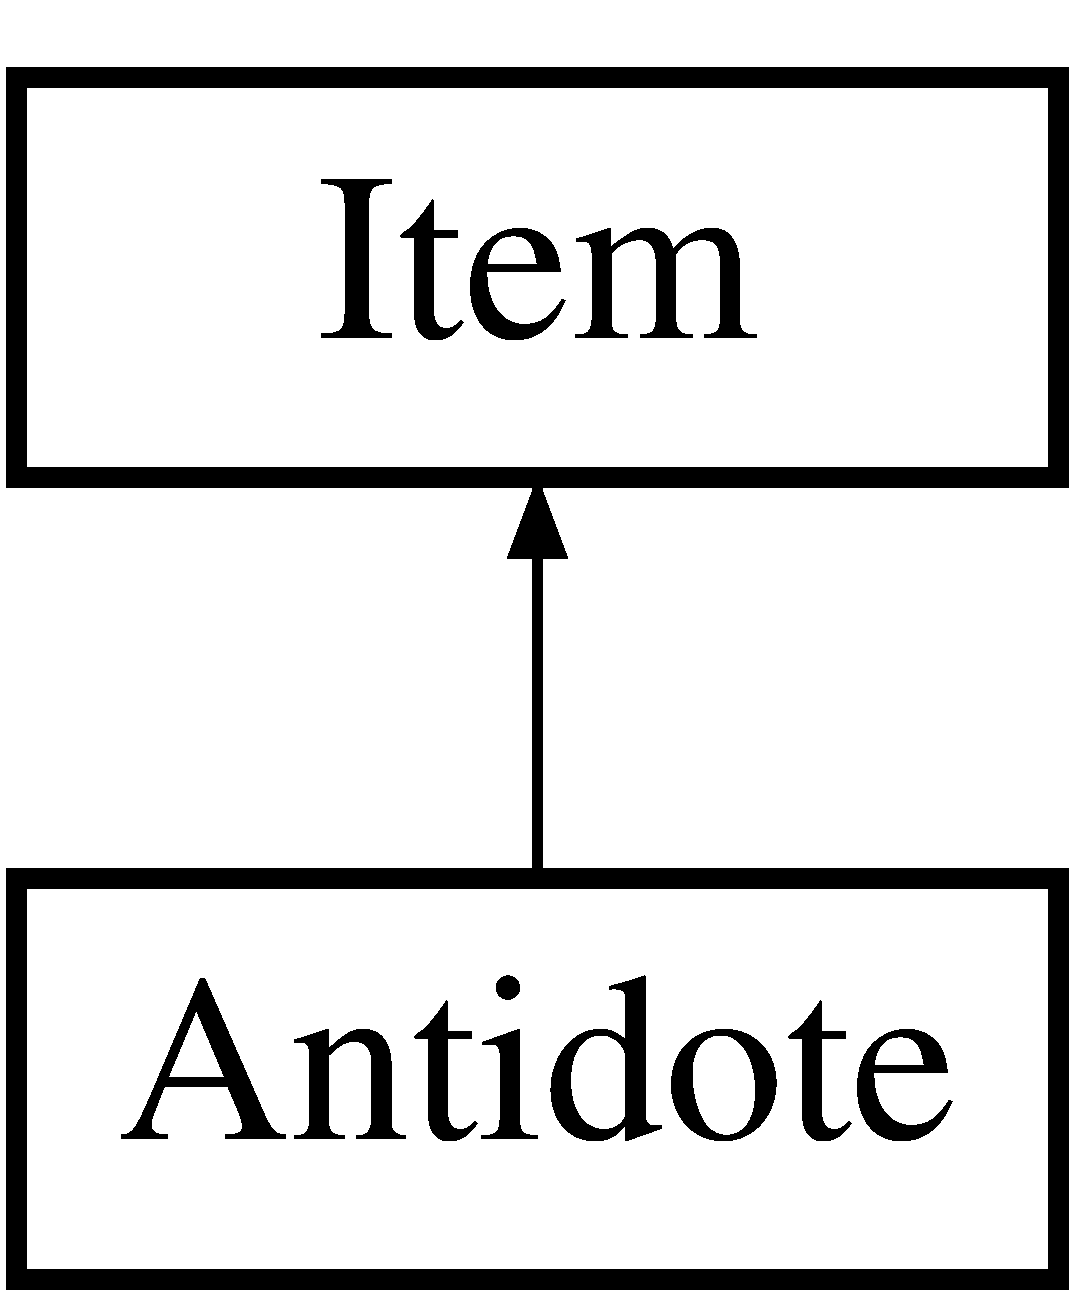
\includegraphics[height=2.000000cm]{class_antidote}
\end{center}
\end{figure}
\subsection*{Public Member Functions}
\begin{DoxyCompactItemize}
\item 
\hypertarget{class_antidote_af9e842ead3c6fbab1147056647ec0ced}{}\hyperlink{class_antidote_af9e842ead3c6fbab1147056647ec0ced}{Antidote} (string name)\label{class_antidote_af9e842ead3c6fbab1147056647ec0ced}

\begin{DoxyCompactList}\small\item\em Constructs an object \hyperlink{class_antidote}{Antidote}. \end{DoxyCompactList}\item 
\hypertarget{class_antidote_af984adccc80a2f49791d6bdfd4918201}{}\hyperlink{class_item}{Item} $\ast$ \hyperlink{class_antidote_af984adccc80a2f49791d6bdfd4918201}{clone} (string name)\label{class_antidote_af984adccc80a2f49791d6bdfd4918201}

\begin{DoxyCompactList}\small\item\em Return a new object \hyperlink{class_antidote}{Antidote}. \end{DoxyCompactList}\end{DoxyCompactItemize}
\subsection*{Additional Inherited Members}


\subsection{Detailed Description}
An \hyperlink{class_antidote}{Antidote} class. 

\hyperlink{class_antidote}{Antidote} class inherited from \hyperlink{class_item}{Item} class. It contains a constructor and a clone function. It is used to cure the player from poison. 

The documentation for this class was generated from the following files\+:\begin{DoxyCompactItemize}
\item 
C\+:/\+Users/\+Mook T/\+Desktop/item/Item\+Prototype.\+h\item 
C\+:/\+Users/\+Mook T/\+Desktop/item/Item\+Prototype.\+cpp\end{DoxyCompactItemize}

\hypertarget{struct_json_1_1_built_styled_stream_writer}{}\section{Json\+:\+:Built\+Styled\+Stream\+Writer Struct Reference}
\label{struct_json_1_1_built_styled_stream_writer}\index{Json\+::\+Built\+Styled\+Stream\+Writer@{Json\+::\+Built\+Styled\+Stream\+Writer}}
Inheritance diagram for Json\+:\+:Built\+Styled\+Stream\+Writer\+:\begin{figure}[H]
\begin{center}
\leavevmode
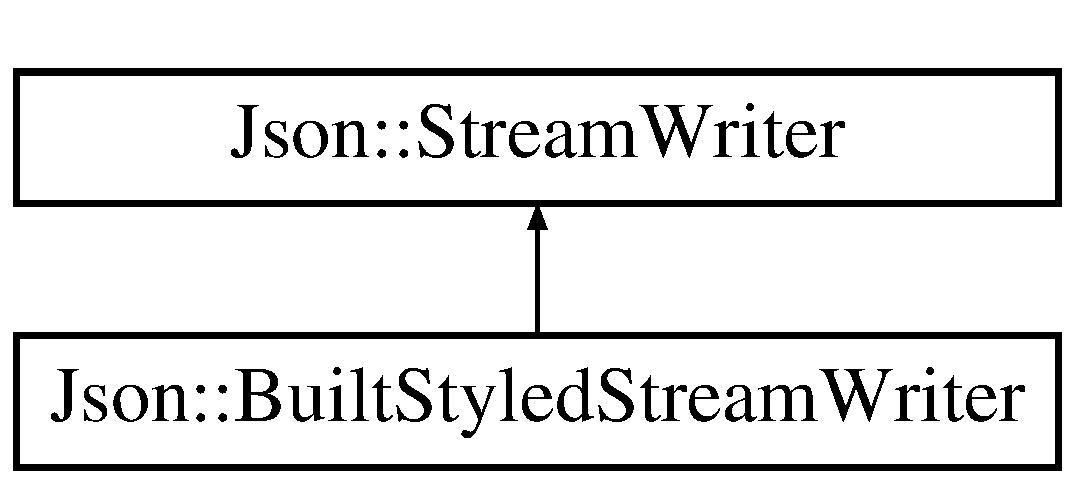
\includegraphics[height=2.000000cm]{struct_json_1_1_built_styled_stream_writer}
\end{center}
\end{figure}
\subsection*{Public Member Functions}
\begin{DoxyCompactItemize}
\item 
\hypertarget{struct_json_1_1_built_styled_stream_writer_ab0c2e665c86b22f8fafb0e52c8069954}{}{\bfseries Built\+Styled\+Stream\+Writer} (std\+::string const \&indentation, \hyperlink{struct_json_1_1_comment_style_a51fc08f3518fd81eba12f340d19a3d0c}{Comment\+Style\+::\+Enum} cs, std\+::string const \&colon\+Symbol, std\+::string const \&null\+Symbol, std\+::string const \&ending\+Line\+Feed\+Symbol, bool use\+Special\+Floats, unsigned int precision)\label{struct_json_1_1_built_styled_stream_writer_ab0c2e665c86b22f8fafb0e52c8069954}

\item 
int \hyperlink{struct_json_1_1_built_styled_stream_writer_ab8810d938c35c8442cbffcd001628cd0}{write} (\hyperlink{class_json_1_1_value}{Value} const \&root, std\+::ostream $\ast$sout)
\end{DoxyCompactItemize}
\subsection*{Private Types}
\begin{DoxyCompactItemize}
\item 
\hypertarget{struct_json_1_1_built_styled_stream_writer_a8356597862a354bcd55a7cb6e0512899}{}typedef std\+::vector$<$ std\+::string $>$ {\bfseries Child\+Values}\label{struct_json_1_1_built_styled_stream_writer_a8356597862a354bcd55a7cb6e0512899}

\end{DoxyCompactItemize}
\subsection*{Private Member Functions}
\begin{DoxyCompactItemize}
\item 
\hypertarget{struct_json_1_1_built_styled_stream_writer_a7c9da861861e570a51b45f270c9ff150}{}void {\bfseries write\+Value} (\hyperlink{class_json_1_1_value}{Value} const \&value)\label{struct_json_1_1_built_styled_stream_writer_a7c9da861861e570a51b45f270c9ff150}

\item 
\hypertarget{struct_json_1_1_built_styled_stream_writer_acd20e9274bbcf7876ef3af2e7d23a31f}{}void {\bfseries write\+Array\+Value} (\hyperlink{class_json_1_1_value}{Value} const \&value)\label{struct_json_1_1_built_styled_stream_writer_acd20e9274bbcf7876ef3af2e7d23a31f}

\item 
\hypertarget{struct_json_1_1_built_styled_stream_writer_af423fd33b3d580506ea3efc53b05a077}{}bool {\bfseries is\+Multine\+Array} (\hyperlink{class_json_1_1_value}{Value} const \&value)\label{struct_json_1_1_built_styled_stream_writer_af423fd33b3d580506ea3efc53b05a077}

\item 
\hypertarget{struct_json_1_1_built_styled_stream_writer_a53de0fe57c883d621c7255e49248651e}{}void {\bfseries push\+Value} (std\+::string const \&value)\label{struct_json_1_1_built_styled_stream_writer_a53de0fe57c883d621c7255e49248651e}

\item 
\hypertarget{struct_json_1_1_built_styled_stream_writer_a2b38a3714d415c4bd3b4812897130f3d}{}void {\bfseries write\+Indent} ()\label{struct_json_1_1_built_styled_stream_writer_a2b38a3714d415c4bd3b4812897130f3d}

\item 
\hypertarget{struct_json_1_1_built_styled_stream_writer_a764c6d530b5bd660c4a7d1ad4eff6b8d}{}void {\bfseries write\+With\+Indent} (std\+::string const \&value)\label{struct_json_1_1_built_styled_stream_writer_a764c6d530b5bd660c4a7d1ad4eff6b8d}

\item 
\hypertarget{struct_json_1_1_built_styled_stream_writer_a73e09692a2cfbd6e67836b060dc34a9f}{}void {\bfseries indent} ()\label{struct_json_1_1_built_styled_stream_writer_a73e09692a2cfbd6e67836b060dc34a9f}

\item 
\hypertarget{struct_json_1_1_built_styled_stream_writer_a0da6c6f603e00c8c6e38af553edd8c55}{}void {\bfseries unindent} ()\label{struct_json_1_1_built_styled_stream_writer_a0da6c6f603e00c8c6e38af553edd8c55}

\item 
\hypertarget{struct_json_1_1_built_styled_stream_writer_a32c4afca4e08fba79bb0a80a8010283a}{}void {\bfseries write\+Comment\+Before\+Value} (\hyperlink{class_json_1_1_value}{Value} const \&root)\label{struct_json_1_1_built_styled_stream_writer_a32c4afca4e08fba79bb0a80a8010283a}

\item 
\hypertarget{struct_json_1_1_built_styled_stream_writer_a89625b134fce0255263ca40e6125742b}{}void {\bfseries write\+Comment\+After\+Value\+On\+Same\+Line} (\hyperlink{class_json_1_1_value}{Value} const \&root)\label{struct_json_1_1_built_styled_stream_writer_a89625b134fce0255263ca40e6125742b}

\end{DoxyCompactItemize}
\subsection*{Static Private Member Functions}
\begin{DoxyCompactItemize}
\item 
\hypertarget{struct_json_1_1_built_styled_stream_writer_a457c2f3c1e8c952caeb60e52477d0c9a}{}static bool {\bfseries has\+Comment\+For\+Value} (const \hyperlink{class_json_1_1_value}{Value} \&value)\label{struct_json_1_1_built_styled_stream_writer_a457c2f3c1e8c952caeb60e52477d0c9a}

\end{DoxyCompactItemize}
\subsection*{Private Attributes}
\begin{DoxyCompactItemize}
\item 
\hypertarget{struct_json_1_1_built_styled_stream_writer_a47d562d7874c5b1e68995bd62f575792}{}Child\+Values {\bfseries child\+Values\+\_\+}\label{struct_json_1_1_built_styled_stream_writer_a47d562d7874c5b1e68995bd62f575792}

\item 
\hypertarget{struct_json_1_1_built_styled_stream_writer_a2abfd5beb7f33adc3f690ce4f618aa2f}{}std\+::string {\bfseries indent\+String\+\_\+}\label{struct_json_1_1_built_styled_stream_writer_a2abfd5beb7f33adc3f690ce4f618aa2f}

\item 
\hypertarget{struct_json_1_1_built_styled_stream_writer_a3a0b46b31273cf61cf3564fba28ea03b}{}int {\bfseries right\+Margin\+\_\+}\label{struct_json_1_1_built_styled_stream_writer_a3a0b46b31273cf61cf3564fba28ea03b}

\item 
\hypertarget{struct_json_1_1_built_styled_stream_writer_ab1d7561ca0f480cb46cc113e1005e8ac}{}std\+::string {\bfseries indentation\+\_\+}\label{struct_json_1_1_built_styled_stream_writer_ab1d7561ca0f480cb46cc113e1005e8ac}

\item 
\hypertarget{struct_json_1_1_built_styled_stream_writer_a89a9c76c7531143b52785861ba21c1d4}{}\hyperlink{struct_json_1_1_comment_style_a51fc08f3518fd81eba12f340d19a3d0c}{Comment\+Style\+::\+Enum} {\bfseries cs\+\_\+}\label{struct_json_1_1_built_styled_stream_writer_a89a9c76c7531143b52785861ba21c1d4}

\item 
\hypertarget{struct_json_1_1_built_styled_stream_writer_ac28b111b1c3ecc1ea6d981c8530ceca4}{}std\+::string {\bfseries colon\+Symbol\+\_\+}\label{struct_json_1_1_built_styled_stream_writer_ac28b111b1c3ecc1ea6d981c8530ceca4}

\item 
\hypertarget{struct_json_1_1_built_styled_stream_writer_a238a8f4737c9835af78ea80cc4f12658}{}std\+::string {\bfseries null\+Symbol\+\_\+}\label{struct_json_1_1_built_styled_stream_writer_a238a8f4737c9835af78ea80cc4f12658}

\item 
\hypertarget{struct_json_1_1_built_styled_stream_writer_a85a8c0e3c9deb2503d497f61bc0da74c}{}std\+::string {\bfseries ending\+Line\+Feed\+Symbol\+\_\+}\label{struct_json_1_1_built_styled_stream_writer_a85a8c0e3c9deb2503d497f61bc0da74c}

\item 
\hypertarget{struct_json_1_1_built_styled_stream_writer_abed9cc31da503b48798e7cea68c42e16}{}bool {\bfseries add\+Child\+Values\+\_\+}\+: 1\label{struct_json_1_1_built_styled_stream_writer_abed9cc31da503b48798e7cea68c42e16}

\item 
\hypertarget{struct_json_1_1_built_styled_stream_writer_a6aa0ad023e623f600103631a6bca6d10}{}bool {\bfseries indented\+\_\+}\+: 1\label{struct_json_1_1_built_styled_stream_writer_a6aa0ad023e623f600103631a6bca6d10}

\item 
\hypertarget{struct_json_1_1_built_styled_stream_writer_a6f1b8694b4eb17ab8c34f6d6dd8c8a4a}{}bool {\bfseries use\+Special\+Floats\+\_\+}\+: 1\label{struct_json_1_1_built_styled_stream_writer_a6f1b8694b4eb17ab8c34f6d6dd8c8a4a}

\item 
\hypertarget{struct_json_1_1_built_styled_stream_writer_a6373d8d0ae4741b64e3904e4db0eef46}{}unsigned int {\bfseries precision\+\_\+}\label{struct_json_1_1_built_styled_stream_writer_a6373d8d0ae4741b64e3904e4db0eef46}

\end{DoxyCompactItemize}
\subsection*{Additional Inherited Members}


\subsection{Member Function Documentation}
\hypertarget{struct_json_1_1_built_styled_stream_writer_ab8810d938c35c8442cbffcd001628cd0}{}\index{Json\+::\+Built\+Styled\+Stream\+Writer@{Json\+::\+Built\+Styled\+Stream\+Writer}!write@{write}}
\index{write@{write}!Json\+::\+Built\+Styled\+Stream\+Writer@{Json\+::\+Built\+Styled\+Stream\+Writer}}
\subsubsection[{write(\+Value const \&root, std\+::ostream $\ast$sout)}]{\setlength{\rightskip}{0pt plus 5cm}int Json\+::\+Built\+Styled\+Stream\+Writer\+::write (
\begin{DoxyParamCaption}
\item[{{\bf Value} const \&}]{root, }
\item[{std\+::ostream $\ast$}]{sout}
\end{DoxyParamCaption}
)\hspace{0.3cm}{\ttfamily [virtual]}}\label{struct_json_1_1_built_styled_stream_writer_ab8810d938c35c8442cbffcd001628cd0}
Write \hyperlink{class_json_1_1_value}{Value} into document as configured in sub-\/class. Do not take ownership of sout, but maintain a reference during function. \begin{DoxyPrecond}{Precondition}
sout != N\+U\+L\+L 
\end{DoxyPrecond}
\begin{DoxyReturn}{Returns}
zero on success (For now, we always return zero, so check the stream instead.) 
\end{DoxyReturn}

\begin{DoxyExceptions}{Exceptions}
{\em std\+::exception} & possibly, depending on configuration \\
\hline
\end{DoxyExceptions}


Implements \hyperlink{class_json_1_1_stream_writer_a237368cf13b41decc015640d25f176ab}{Json\+::\+Stream\+Writer}.



The documentation for this struct was generated from the following file\+:\begin{DoxyCompactItemize}
\item 
C\+:/\+Users/\+Mook T/\+Desktop/item/jsoncpp.\+cpp\end{DoxyCompactItemize}

\hypertarget{class_json_1_1_char_reader}{}\section{Json\+:\+:Char\+Reader Class Reference}
\label{class_json_1_1_char_reader}\index{Json\+::\+Char\+Reader@{Json\+::\+Char\+Reader}}


{\ttfamily \#include $<$json.\+h$>$}

Inheritance diagram for Json\+:\+:Char\+Reader\+:\begin{figure}[H]
\begin{center}
\leavevmode
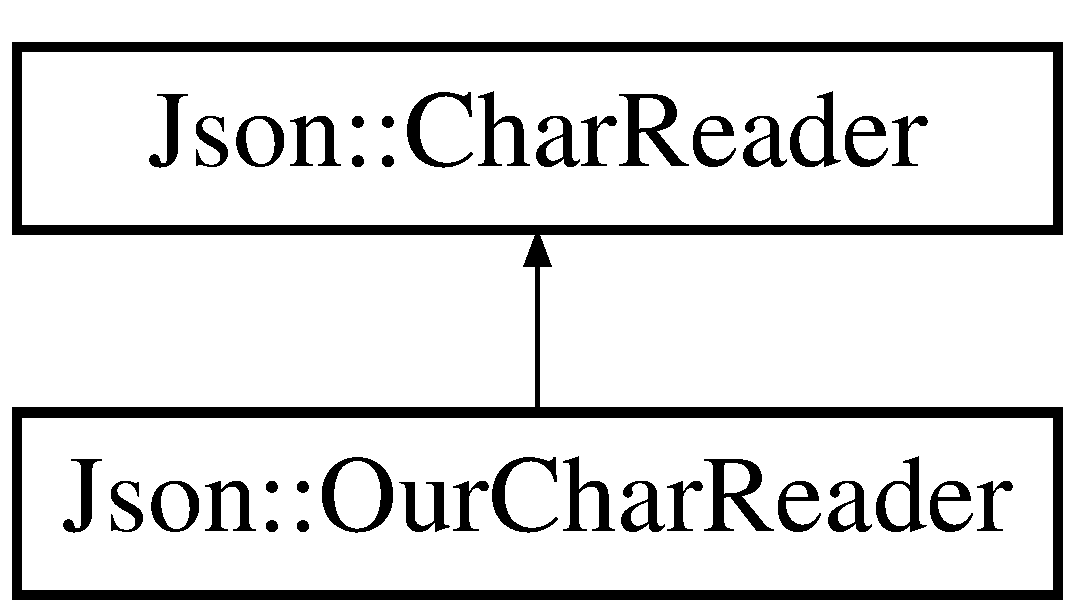
\includegraphics[height=2.000000cm]{class_json_1_1_char_reader}
\end{center}
\end{figure}
\subsection*{Classes}
\begin{DoxyCompactItemize}
\item 
class \hyperlink{class_json_1_1_char_reader_1_1_factory}{Factory}
\end{DoxyCompactItemize}
\subsection*{Public Member Functions}
\begin{DoxyCompactItemize}
\item 
virtual bool \hyperlink{class_json_1_1_char_reader_a48e320be8b13bbc0960cc5808cafec98}{parse} (char const $\ast$begin\+Doc, char const $\ast$end\+Doc, \hyperlink{class_json_1_1_value}{Value} $\ast$root, std\+::string $\ast$errs)=0
\begin{DoxyCompactList}\small\item\em Read a \hyperlink{class_json_1_1_value}{Value} from a \href{http://www.json.org}{\tt J\+S\+O\+N} document. The document must be a U\+T\+F-\/8 encoded string containing the document to read. \end{DoxyCompactList}\end{DoxyCompactItemize}


\subsection{Detailed Description}
Interface for reading J\+S\+O\+N from a char array. 

\subsection{Member Function Documentation}
\hypertarget{class_json_1_1_char_reader_a48e320be8b13bbc0960cc5808cafec98}{}\index{Json\+::\+Char\+Reader@{Json\+::\+Char\+Reader}!parse@{parse}}
\index{parse@{parse}!Json\+::\+Char\+Reader@{Json\+::\+Char\+Reader}}
\subsubsection[{parse(char const $\ast$begin\+Doc, char const $\ast$end\+Doc, Value $\ast$root, std\+::string $\ast$errs)=0}]{\setlength{\rightskip}{0pt plus 5cm}virtual bool Json\+::\+Char\+Reader\+::parse (
\begin{DoxyParamCaption}
\item[{char const $\ast$}]{begin\+Doc, }
\item[{char const $\ast$}]{end\+Doc, }
\item[{{\bf Value} $\ast$}]{root, }
\item[{std\+::string $\ast$}]{errs}
\end{DoxyParamCaption}
)\hspace{0.3cm}{\ttfamily [pure virtual]}}\label{class_json_1_1_char_reader_a48e320be8b13bbc0960cc5808cafec98}


Read a \hyperlink{class_json_1_1_value}{Value} from a \href{http://www.json.org}{\tt J\+S\+O\+N} document. The document must be a U\+T\+F-\/8 encoded string containing the document to read. 


\begin{DoxyParams}{Parameters}
{\em begin\+Doc} & Pointer on the beginning of the U\+T\+F-\/8 encoded string of the document to read. \\
\hline
{\em end\+Doc} & Pointer on the end of the U\+T\+F-\/8 encoded string of the document to read. Must be $>$= begin\+Doc. \\
\hline
{\em root} & \mbox{[}out\mbox{]} Contains the root value of the document if it was successfully parsed. \\
\hline
{\em errs} & \mbox{[}out\mbox{]} Formatted error messages (if not N\+U\+L\+L) a user friendly string that lists errors in the parsed document. \\
\hline
\end{DoxyParams}
\begin{DoxyReturn}{Returns}
{\ttfamily true} if the document was successfully parsed, {\ttfamily false} if an error occurred. 
\end{DoxyReturn}


Implemented in \hyperlink{class_json_1_1_our_char_reader_a268b63f96796d6acea7053fc7c83b05d}{Json\+::\+Our\+Char\+Reader}.



The documentation for this class was generated from the following file\+:\begin{DoxyCompactItemize}
\item 
C\+:/\+Users/\+Mook T/\+Desktop/item/json.\+h\end{DoxyCompactItemize}

\hypertarget{class_json_1_1_char_reader_builder}{}\section{Json\+:\+:Char\+Reader\+Builder Class Reference}
\label{class_json_1_1_char_reader_builder}\index{Json\+::\+Char\+Reader\+Builder@{Json\+::\+Char\+Reader\+Builder}}


Build a \hyperlink{class_json_1_1_char_reader}{Char\+Reader} implementation.  




{\ttfamily \#include $<$json.\+h$>$}

Inheritance diagram for Json\+:\+:Char\+Reader\+Builder\+:\begin{figure}[H]
\begin{center}
\leavevmode
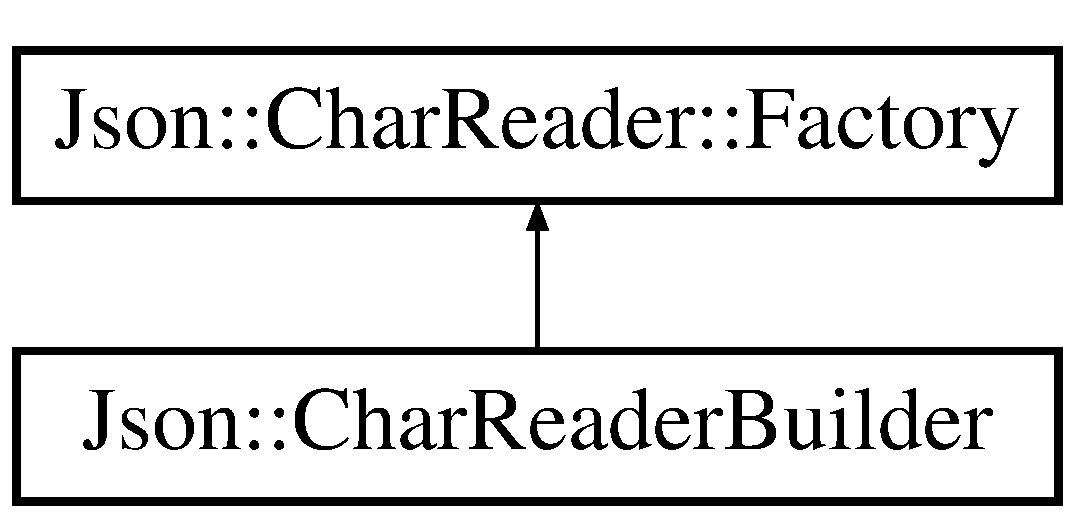
\includegraphics[height=2.000000cm]{class_json_1_1_char_reader_builder}
\end{center}
\end{figure}
\subsection*{Public Member Functions}
\begin{DoxyCompactItemize}
\item 
\hyperlink{class_json_1_1_char_reader}{Char\+Reader} $\ast$ \hyperlink{class_json_1_1_char_reader_builder_a3e3c9f4aeb07023ef0c5f6255003078a}{new\+Char\+Reader} () const 
\begin{DoxyCompactList}\small\item\em Allocate a \hyperlink{class_json_1_1_char_reader}{Char\+Reader} via operator new(). \end{DoxyCompactList}\item 
bool \hyperlink{class_json_1_1_char_reader_builder_a3d233735a1e4b3c9a2cb9c68f972c02a}{validate} (\hyperlink{class_json_1_1_value}{Json\+::\+Value} $\ast$invalid) const 
\item 
\hyperlink{class_json_1_1_value}{Value} \& \hyperlink{class_json_1_1_char_reader_builder_a324561448113b48eb7aa6e6a5ce3aa0d}{operator\mbox{[}$\,$\mbox{]}} (std\+::string key)
\end{DoxyCompactItemize}
\subsection*{Static Public Member Functions}
\begin{DoxyCompactItemize}
\item 
static void \hyperlink{class_json_1_1_char_reader_builder_a03ff031e06aabff989ab4addc87294ab}{set\+Defaults} (\hyperlink{class_json_1_1_value}{Json\+::\+Value} $\ast$settings)
\item 
static void \hyperlink{class_json_1_1_char_reader_builder_a9c19e3c5475f9072d527810d4bf56749}{strict\+Mode} (\hyperlink{class_json_1_1_value}{Json\+::\+Value} $\ast$settings)
\end{DoxyCompactItemize}
\subsection*{Public Attributes}
\begin{DoxyCompactItemize}
\item 
\hyperlink{class_json_1_1_value}{Json\+::\+Value} \hyperlink{class_json_1_1_char_reader_builder_ac69b7911ad64c171c51ebaf2ea26d958}{settings\+\_\+}
\end{DoxyCompactItemize}


\subsection{Detailed Description}
Build a \hyperlink{class_json_1_1_char_reader}{Char\+Reader} implementation. 

Usage\+: 
\begin{DoxyCode}
\textcolor{keyword}{using namespace }\hyperlink{namespace_json}{Json};
\hyperlink{class_json_1_1_char_reader_builder}{CharReaderBuilder} builder;
builder[\textcolor{stringliteral}{"collectComments"}] = \textcolor{keyword}{false};
\hyperlink{class_json_1_1_value}{Value} value;
std::string errs;
\textcolor{keywordtype}{bool} ok = \hyperlink{namespace_json_acfebeaf759a841173ddce34c4da22486}{parseFromStream}(builder, std::cin, &value, &errs);
\end{DoxyCode}
 

\subsection{Member Function Documentation}
\hypertarget{class_json_1_1_char_reader_builder_a3e3c9f4aeb07023ef0c5f6255003078a}{}\index{Json\+::\+Char\+Reader\+Builder@{Json\+::\+Char\+Reader\+Builder}!new\+Char\+Reader@{new\+Char\+Reader}}
\index{new\+Char\+Reader@{new\+Char\+Reader}!Json\+::\+Char\+Reader\+Builder@{Json\+::\+Char\+Reader\+Builder}}
\subsubsection[{new\+Char\+Reader() const }]{\setlength{\rightskip}{0pt plus 5cm}{\bf Char\+Reader} $\ast$ Json\+::\+Char\+Reader\+Builder\+::new\+Char\+Reader (
\begin{DoxyParamCaption}
{}
\end{DoxyParamCaption}
) const\hspace{0.3cm}{\ttfamily [virtual]}}\label{class_json_1_1_char_reader_builder_a3e3c9f4aeb07023ef0c5f6255003078a}


Allocate a \hyperlink{class_json_1_1_char_reader}{Char\+Reader} via operator new(). 


\begin{DoxyExceptions}{Exceptions}
{\em std\+::exception} & if something goes wrong (e.\+g. invalid settings) \\
\hline
\end{DoxyExceptions}


Implements \hyperlink{class_json_1_1_char_reader_1_1_factory_a497112c51f36a676aeb496c3a91d38d0}{Json\+::\+Char\+Reader\+::\+Factory}.

\hypertarget{class_json_1_1_char_reader_builder_a324561448113b48eb7aa6e6a5ce3aa0d}{}\index{Json\+::\+Char\+Reader\+Builder@{Json\+::\+Char\+Reader\+Builder}!operator\mbox{[}$\,$\mbox{]}@{operator[]}}
\index{operator\mbox{[}$\,$\mbox{]}@{operator[]}!Json\+::\+Char\+Reader\+Builder@{Json\+::\+Char\+Reader\+Builder}}
\subsubsection[{operator[](std\+::string key)}]{\setlength{\rightskip}{0pt plus 5cm}{\bf Value} \& Json\+::\+Char\+Reader\+Builder\+::operator\mbox{[}$\,$\mbox{]} (
\begin{DoxyParamCaption}
\item[{std\+::string}]{key}
\end{DoxyParamCaption}
)}\label{class_json_1_1_char_reader_builder_a324561448113b48eb7aa6e6a5ce3aa0d}
A simple way to update a specific setting. \hypertarget{class_json_1_1_char_reader_builder_a03ff031e06aabff989ab4addc87294ab}{}\index{Json\+::\+Char\+Reader\+Builder@{Json\+::\+Char\+Reader\+Builder}!set\+Defaults@{set\+Defaults}}
\index{set\+Defaults@{set\+Defaults}!Json\+::\+Char\+Reader\+Builder@{Json\+::\+Char\+Reader\+Builder}}
\subsubsection[{set\+Defaults(\+Json\+::\+Value $\ast$settings)}]{\setlength{\rightskip}{0pt plus 5cm}void Json\+::\+Char\+Reader\+Builder\+::set\+Defaults (
\begin{DoxyParamCaption}
\item[{{\bf Json\+::\+Value} $\ast$}]{settings}
\end{DoxyParamCaption}
)\hspace{0.3cm}{\ttfamily [static]}}\label{class_json_1_1_char_reader_builder_a03ff031e06aabff989ab4addc87294ab}
Called by ctor, but you can use this to reset settings\+\_\+. \begin{DoxyPrecond}{Precondition}
\textquotesingle{}settings\textquotesingle{} != N\+U\+L\+L (but Json\+::null is fine) 
\end{DoxyPrecond}
\begin{DoxyRemark}{Remarks}
Defaults\+: 
\begin{DoxyCodeInclude}
\end{DoxyCodeInclude}

\end{DoxyRemark}
\mbox{[}Char\+Reader\+Builder\+Defaults\mbox{]}

\mbox{[}Char\+Reader\+Builder\+Defaults\mbox{]} \hypertarget{class_json_1_1_char_reader_builder_a9c19e3c5475f9072d527810d4bf56749}{}\index{Json\+::\+Char\+Reader\+Builder@{Json\+::\+Char\+Reader\+Builder}!strict\+Mode@{strict\+Mode}}
\index{strict\+Mode@{strict\+Mode}!Json\+::\+Char\+Reader\+Builder@{Json\+::\+Char\+Reader\+Builder}}
\subsubsection[{strict\+Mode(\+Json\+::\+Value $\ast$settings)}]{\setlength{\rightskip}{0pt plus 5cm}void Json\+::\+Char\+Reader\+Builder\+::strict\+Mode (
\begin{DoxyParamCaption}
\item[{{\bf Json\+::\+Value} $\ast$}]{settings}
\end{DoxyParamCaption}
)\hspace{0.3cm}{\ttfamily [static]}}\label{class_json_1_1_char_reader_builder_a9c19e3c5475f9072d527810d4bf56749}
Same as old \hyperlink{class_json_1_1_features_ae23176c14b2e79e81fb61fb1a8ab58ee}{Features\+::strict\+Mode()}. \begin{DoxyPrecond}{Precondition}
\textquotesingle{}settings\textquotesingle{} != N\+U\+L\+L (but Json\+::null is fine) 
\end{DoxyPrecond}
\begin{DoxyRemark}{Remarks}
Defaults\+: 
\begin{DoxyCodeInclude}
\end{DoxyCodeInclude}

\end{DoxyRemark}
\mbox{[}Char\+Reader\+Builder\+Strict\+Mode\mbox{]}

\mbox{[}Char\+Reader\+Builder\+Strict\+Mode\mbox{]} \hypertarget{class_json_1_1_char_reader_builder_a3d233735a1e4b3c9a2cb9c68f972c02a}{}\index{Json\+::\+Char\+Reader\+Builder@{Json\+::\+Char\+Reader\+Builder}!validate@{validate}}
\index{validate@{validate}!Json\+::\+Char\+Reader\+Builder@{Json\+::\+Char\+Reader\+Builder}}
\subsubsection[{validate(\+Json\+::\+Value $\ast$invalid) const }]{\setlength{\rightskip}{0pt plus 5cm}bool Json\+::\+Char\+Reader\+Builder\+::validate (
\begin{DoxyParamCaption}
\item[{{\bf Json\+::\+Value} $\ast$}]{invalid}
\end{DoxyParamCaption}
) const}\label{class_json_1_1_char_reader_builder_a3d233735a1e4b3c9a2cb9c68f972c02a}
\begin{DoxyReturn}{Returns}
true if \textquotesingle{}settings\textquotesingle{} are legal and consistent; otherwise, indicate bad settings via \textquotesingle{}invalid\textquotesingle{}. 
\end{DoxyReturn}


\subsection{Member Data Documentation}
\hypertarget{class_json_1_1_char_reader_builder_ac69b7911ad64c171c51ebaf2ea26d958}{}\index{Json\+::\+Char\+Reader\+Builder@{Json\+::\+Char\+Reader\+Builder}!settings\+\_\+@{settings\+\_\+}}
\index{settings\+\_\+@{settings\+\_\+}!Json\+::\+Char\+Reader\+Builder@{Json\+::\+Char\+Reader\+Builder}}
\subsubsection[{settings\+\_\+}]{\setlength{\rightskip}{0pt plus 5cm}{\bf Json\+::\+Value} Json\+::\+Char\+Reader\+Builder\+::settings\+\_\+}\label{class_json_1_1_char_reader_builder_ac69b7911ad64c171c51ebaf2ea26d958}
Configuration of this builder. These are case-\/sensitive. Available settings (case-\/sensitive)\+:
\begin{DoxyItemize}
\item {\ttfamily \char`\"{}collect\+Comments\char`\"{}\+: false or true}
\begin{DoxyItemize}
\item true to collect comment and allow writing them back during serialization, false to discard comments. This parameter is ignored if allow\+Comments is false.
\end{DoxyItemize}
\item {\ttfamily \char`\"{}allow\+Comments\char`\"{}\+: false or true}
\begin{DoxyItemize}
\item true if comments are allowed.
\end{DoxyItemize}
\item {\ttfamily \char`\"{}strict\+Root\char`\"{}\+: false or true}
\begin{DoxyItemize}
\item true if root must be either an array or an object value
\end{DoxyItemize}
\item {\ttfamily \char`\"{}allow\+Dropped\+Null\+Placeholders\char`\"{}\+: false or true}
\begin{DoxyItemize}
\item true if dropped null placeholders are allowed. (See \hyperlink{class_json_1_1_stream_writer_builder}{Stream\+Writer\+Builder}.)
\end{DoxyItemize}
\item {\ttfamily \char`\"{}allow\+Numeric\+Keys\char`\"{}\+: false or true}
\begin{DoxyItemize}
\item true if numeric object keys are allowed.
\end{DoxyItemize}
\item {\ttfamily \char`\"{}allow\+Single\+Quotes\char`\"{}\+: false or true}
\begin{DoxyItemize}
\item true if \textquotesingle{}\textquotesingle{} are allowed for strings (both keys and values)
\end{DoxyItemize}
\item {\ttfamily \char`\"{}stack\+Limit\char`\"{}\+: integer}
\begin{DoxyItemize}
\item Exceeding stack\+Limit (recursive depth of {\ttfamily read\+Value()}) will cause an exception.
\item This is a security issue (seg-\/faults caused by deeply nested J\+S\+O\+N), so the default is low.
\end{DoxyItemize}
\item {\ttfamily \char`\"{}fail\+If\+Extra\char`\"{}\+: false or true}
\begin{DoxyItemize}
\item If true, {\ttfamily parse()} returns false when extra non-\/whitespace trails the J\+S\+O\+N value in the input string.
\end{DoxyItemize}
\item {\ttfamily \char`\"{}reject\+Dup\+Keys\char`\"{}\+: false or true}
\begin{DoxyItemize}
\item If true, {\ttfamily parse()} returns false when a key is duplicated within an object.
\end{DoxyItemize}
\item {\ttfamily \char`\"{}allow\+Special\+Floats\char`\"{}\+: false or true}
\begin{DoxyItemize}
\item If true, special float values (Na\+Ns and infinities) are allowed and their values are lossfree restorable.
\end{DoxyItemize}
\end{DoxyItemize}

You can examine \textquotesingle{}settings\+\_\+` yourself to see the defaults. You can also write and read them just like any J\+S\+O\+N \hyperlink{class_json_1_1_value}{Value}. \begin{DoxySeeAlso}{See also}
\hyperlink{class_json_1_1_char_reader_builder_a03ff031e06aabff989ab4addc87294ab}{set\+Defaults()} 
\end{DoxySeeAlso}


The documentation for this class was generated from the following files\+:\begin{DoxyCompactItemize}
\item 
C\+:/\+Users/\+Mook T/\+Desktop/item/json.\+h\item 
C\+:/\+Users/\+Mook T/\+Desktop/item/jsoncpp.\+cpp\end{DoxyCompactItemize}

\hypertarget{struct_json_1_1_value_1_1_comment_info}{}\section{Json\+:\+:Value\+:\+:Comment\+Info Struct Reference}
\label{struct_json_1_1_value_1_1_comment_info}\index{Json\+::\+Value\+::\+Comment\+Info@{Json\+::\+Value\+::\+Comment\+Info}}
\subsection*{Public Member Functions}
\begin{DoxyCompactItemize}
\item 
\hypertarget{struct_json_1_1_value_1_1_comment_info_a4d01c2cd8c07995969c5d636dfd4fa8c}{}void {\bfseries set\+Comment} (const char $\ast$text, size\+\_\+t len)\label{struct_json_1_1_value_1_1_comment_info_a4d01c2cd8c07995969c5d636dfd4fa8c}

\end{DoxyCompactItemize}
\subsection*{Public Attributes}
\begin{DoxyCompactItemize}
\item 
\hypertarget{struct_json_1_1_value_1_1_comment_info_a020f19c7098bab8ec8fec14cd1a5afb9}{}char $\ast$ {\bfseries comment\+\_\+}\label{struct_json_1_1_value_1_1_comment_info_a020f19c7098bab8ec8fec14cd1a5afb9}

\end{DoxyCompactItemize}


The documentation for this struct was generated from the following files\+:\begin{DoxyCompactItemize}
\item 
C\+:/\+Users/\+Mook T/\+Desktop/item/json.\+h\item 
C\+:/\+Users/\+Mook T/\+Desktop/item/jsoncpp.\+cpp\end{DoxyCompactItemize}

\hypertarget{struct_json_1_1_comment_style}{}\section{Json\+:\+:Comment\+Style Struct Reference}
\label{struct_json_1_1_comment_style}\index{Json\+::\+Comment\+Style@{Json\+::\+Comment\+Style}}


Scoped enums are not available until C++11.  


\subsection*{Public Types}
\begin{DoxyCompactItemize}
\item 
enum \hyperlink{struct_json_1_1_comment_style_a51fc08f3518fd81eba12f340d19a3d0c}{Enum} \{ \hyperlink{struct_json_1_1_comment_style_a51fc08f3518fd81eba12f340d19a3d0cac8b32a8bae63414c8647d4919da8d437}{None}, 
\hyperlink{struct_json_1_1_comment_style_a51fc08f3518fd81eba12f340d19a3d0cac65238f050773c107690a456e9c05c98}{Most}, 
\hyperlink{struct_json_1_1_comment_style_a51fc08f3518fd81eba12f340d19a3d0ca32302c0b97190c1808b3e38f367fef01}{All}
 \}\begin{DoxyCompactList}\small\item\em Decide whether to write comments. \end{DoxyCompactList}
\end{DoxyCompactItemize}


\subsection{Detailed Description}
Scoped enums are not available until C++11. 

\subsection{Member Enumeration Documentation}
\hypertarget{struct_json_1_1_comment_style_a51fc08f3518fd81eba12f340d19a3d0c}{}\index{Json\+::\+Comment\+Style@{Json\+::\+Comment\+Style}!Enum@{Enum}}
\index{Enum@{Enum}!Json\+::\+Comment\+Style@{Json\+::\+Comment\+Style}}
\subsubsection[{Enum}]{\setlength{\rightskip}{0pt plus 5cm}enum {\bf Json\+::\+Comment\+Style\+::\+Enum}}\label{struct_json_1_1_comment_style_a51fc08f3518fd81eba12f340d19a3d0c}


Decide whether to write comments. 

\begin{Desc}
\item[Enumerator]\par
\begin{description}
\index{None@{None}!Json\+::\+Comment\+Style@{Json\+::\+Comment\+Style}}\index{Json\+::\+Comment\+Style@{Json\+::\+Comment\+Style}!None@{None}}\item[{\em 
\hypertarget{struct_json_1_1_comment_style_a51fc08f3518fd81eba12f340d19a3d0cac8b32a8bae63414c8647d4919da8d437}{}None\label{struct_json_1_1_comment_style_a51fc08f3518fd81eba12f340d19a3d0cac8b32a8bae63414c8647d4919da8d437}
}]Drop all comments. \index{Most@{Most}!Json\+::\+Comment\+Style@{Json\+::\+Comment\+Style}}\index{Json\+::\+Comment\+Style@{Json\+::\+Comment\+Style}!Most@{Most}}\item[{\em 
\hypertarget{struct_json_1_1_comment_style_a51fc08f3518fd81eba12f340d19a3d0cac65238f050773c107690a456e9c05c98}{}Most\label{struct_json_1_1_comment_style_a51fc08f3518fd81eba12f340d19a3d0cac65238f050773c107690a456e9c05c98}
}]Recover odd behavior of previous versions (not implemented yet). \index{All@{All}!Json\+::\+Comment\+Style@{Json\+::\+Comment\+Style}}\index{Json\+::\+Comment\+Style@{Json\+::\+Comment\+Style}!All@{All}}\item[{\em 
\hypertarget{struct_json_1_1_comment_style_a51fc08f3518fd81eba12f340d19a3d0ca32302c0b97190c1808b3e38f367fef01}{}All\label{struct_json_1_1_comment_style_a51fc08f3518fd81eba12f340d19a3d0ca32302c0b97190c1808b3e38f367fef01}
}]Keep all comments. \end{description}
\end{Desc}


The documentation for this struct was generated from the following file\+:\begin{DoxyCompactItemize}
\item 
C\+:/\+Users/\+Mook T/\+Desktop/item/jsoncpp.\+cpp\end{DoxyCompactItemize}

\hypertarget{class_json_1_1_value_1_1_c_z_string}{}\section{Json\+:\+:Value\+:\+:C\+Z\+String Class Reference}
\label{class_json_1_1_value_1_1_c_z_string}\index{Json\+::\+Value\+::\+C\+Z\+String@{Json\+::\+Value\+::\+C\+Z\+String}}
\subsection*{Classes}
\begin{DoxyCompactItemize}
\item 
struct \hyperlink{struct_json_1_1_value_1_1_c_z_string_1_1_string_storage}{String\+Storage}
\end{DoxyCompactItemize}
\subsection*{Public Types}
\begin{DoxyCompactItemize}
\item 
\hypertarget{class_json_1_1_value_1_1_c_z_string_a2805c46fb4a72bbaed55de6d75941b6d}{}enum {\bfseries Duplication\+Policy} \{ {\bfseries no\+Duplication} = 0, 
{\bfseries duplicate}, 
{\bfseries duplicate\+On\+Copy}
 \}\label{class_json_1_1_value_1_1_c_z_string_a2805c46fb4a72bbaed55de6d75941b6d}

\end{DoxyCompactItemize}
\subsection*{Public Member Functions}
\begin{DoxyCompactItemize}
\item 
\hypertarget{class_json_1_1_value_1_1_c_z_string_a4b8aa6eaabdec78cffec96e088da996f}{}{\bfseries C\+Z\+String} (Array\+Index index)\label{class_json_1_1_value_1_1_c_z_string_a4b8aa6eaabdec78cffec96e088da996f}

\item 
\hypertarget{class_json_1_1_value_1_1_c_z_string_a86a86eaf0cf26d4c861d0daa359d608a}{}{\bfseries C\+Z\+String} (char const $\ast$str, unsigned length, Duplication\+Policy allocate)\label{class_json_1_1_value_1_1_c_z_string_a86a86eaf0cf26d4c861d0daa359d608a}

\item 
\hypertarget{class_json_1_1_value_1_1_c_z_string_a9685070d440335b55ef5c85747d25157}{}{\bfseries C\+Z\+String} (\hyperlink{class_json_1_1_value_1_1_c_z_string}{C\+Z\+String} const \&other)\label{class_json_1_1_value_1_1_c_z_string_a9685070d440335b55ef5c85747d25157}

\item 
\hypertarget{class_json_1_1_value_1_1_c_z_string_a6513ff431b0593d5744868dfee739f7b}{}\hyperlink{class_json_1_1_value_1_1_c_z_string}{C\+Z\+String} \& {\bfseries operator=} (\hyperlink{class_json_1_1_value_1_1_c_z_string}{C\+Z\+String} other)\label{class_json_1_1_value_1_1_c_z_string_a6513ff431b0593d5744868dfee739f7b}

\item 
\hypertarget{class_json_1_1_value_1_1_c_z_string_a5e88edf9f7443c77d6b70e409a0b5983}{}bool {\bfseries operator$<$} (\hyperlink{class_json_1_1_value_1_1_c_z_string}{C\+Z\+String} const \&other) const \label{class_json_1_1_value_1_1_c_z_string_a5e88edf9f7443c77d6b70e409a0b5983}

\item 
\hypertarget{class_json_1_1_value_1_1_c_z_string_af7a3b51ccf1bb205210c6b9a570093bc}{}bool {\bfseries operator==} (\hyperlink{class_json_1_1_value_1_1_c_z_string}{C\+Z\+String} const \&other) const \label{class_json_1_1_value_1_1_c_z_string_af7a3b51ccf1bb205210c6b9a570093bc}

\item 
\hypertarget{class_json_1_1_value_1_1_c_z_string_a4e9f305dbc4a4700abd955fde673a01c}{}Array\+Index {\bfseries index} () const \label{class_json_1_1_value_1_1_c_z_string_a4e9f305dbc4a4700abd955fde673a01c}

\item 
\hypertarget{class_json_1_1_value_1_1_c_z_string_a02482793b88b1062c4a0dd0a53f3d2a7}{}char const $\ast$ {\bfseries data} () const \label{class_json_1_1_value_1_1_c_z_string_a02482793b88b1062c4a0dd0a53f3d2a7}

\item 
\hypertarget{class_json_1_1_value_1_1_c_z_string_a4e697840c41fb56756be7a75efa114cb}{}unsigned {\bfseries length} () const \label{class_json_1_1_value_1_1_c_z_string_a4e697840c41fb56756be7a75efa114cb}

\item 
\hypertarget{class_json_1_1_value_1_1_c_z_string_af3cc02b77c2cd79d4646fcea3575c1fd}{}bool {\bfseries is\+Static\+String} () const \label{class_json_1_1_value_1_1_c_z_string_af3cc02b77c2cd79d4646fcea3575c1fd}

\end{DoxyCompactItemize}
\subsection*{Private Member Functions}
\begin{DoxyCompactItemize}
\item 
\hypertarget{class_json_1_1_value_1_1_c_z_string_ad59f3542d2eea749a6a63409d1a02207}{}void {\bfseries swap} (\hyperlink{class_json_1_1_value_1_1_c_z_string}{C\+Z\+String} \&other)\label{class_json_1_1_value_1_1_c_z_string_ad59f3542d2eea749a6a63409d1a02207}

\end{DoxyCompactItemize}
\subsection*{Private Attributes}
\begin{DoxyCompactItemize}
\item 
\hypertarget{class_json_1_1_value_1_1_c_z_string_a5b4d28349294034d7f779c3c95d0306c}{}char const $\ast$ {\bfseries cstr\+\_\+}\label{class_json_1_1_value_1_1_c_z_string_a5b4d28349294034d7f779c3c95d0306c}

\item 
\hypertarget{class_json_1_1_value_1_1_c_z_string_a6f6b20ee7c8873fba58100f869ca2e5e}{}\begin{tabbing}
xx\=xx\=xx\=xx\=xx\=xx\=xx\=xx\=xx\=\kill
union \{\\
\>ArrayIndex {\bfseries index\_}\\
\>\hyperlink{struct_json_1_1_value_1_1_c_z_string_1_1_string_storage}{StringStorage} {\bfseries storage\_}\\
\}; \label{class_json_1_1_value_1_1_c_z_string_a6f6b20ee7c8873fba58100f869ca2e5e}
\\

\end{tabbing}\end{DoxyCompactItemize}


The documentation for this class was generated from the following files\+:\begin{DoxyCompactItemize}
\item 
C\+:/\+Users/\+Mook T/\+Desktop/item/json.\+h\item 
C\+:/\+Users/\+Mook T/\+Desktop/item/jsoncpp.\+cpp\end{DoxyCompactItemize}

\hypertarget{class_json_1_1_our_reader_1_1_error_info}{}\section{Json\+:\+:Our\+Reader\+:\+:Error\+Info Class Reference}
\label{class_json_1_1_our_reader_1_1_error_info}\index{Json\+::\+Our\+Reader\+::\+Error\+Info@{Json\+::\+Our\+Reader\+::\+Error\+Info}}
\subsection*{Public Attributes}
\begin{DoxyCompactItemize}
\item 
\hypertarget{class_json_1_1_our_reader_1_1_error_info_ad05204ecabe5e7201a842935b874ae9a}{}\hyperlink{class_json_1_1_our_reader_1_1_token}{Token} {\bfseries token\+\_\+}\label{class_json_1_1_our_reader_1_1_error_info_ad05204ecabe5e7201a842935b874ae9a}

\item 
\hypertarget{class_json_1_1_our_reader_1_1_error_info_a9c973ff4d2c47134b770027d5d37d906}{}std\+::string {\bfseries message\+\_\+}\label{class_json_1_1_our_reader_1_1_error_info_a9c973ff4d2c47134b770027d5d37d906}

\item 
\hypertarget{class_json_1_1_our_reader_1_1_error_info_a77ba2d32a471c7b9bc14621b76a5bdab}{}Location {\bfseries extra\+\_\+}\label{class_json_1_1_our_reader_1_1_error_info_a77ba2d32a471c7b9bc14621b76a5bdab}

\end{DoxyCompactItemize}


The documentation for this class was generated from the following file\+:\begin{DoxyCompactItemize}
\item 
C\+:/\+Users/\+Mook T/\+Desktop/item/jsoncpp.\+cpp\end{DoxyCompactItemize}

\hypertarget{class_json_1_1_reader_1_1_error_info}{}\section{Json\+:\+:Reader\+:\+:Error\+Info Class Reference}
\label{class_json_1_1_reader_1_1_error_info}\index{Json\+::\+Reader\+::\+Error\+Info@{Json\+::\+Reader\+::\+Error\+Info}}
\subsection*{Public Attributes}
\begin{DoxyCompactItemize}
\item 
\hypertarget{class_json_1_1_reader_1_1_error_info_a52e1c71b12eb1c3f0395d7ef1e778ce6}{}\hyperlink{class_json_1_1_reader_1_1_token}{Token} {\bfseries token\+\_\+}\label{class_json_1_1_reader_1_1_error_info_a52e1c71b12eb1c3f0395d7ef1e778ce6}

\item 
\hypertarget{class_json_1_1_reader_1_1_error_info_aeb2fb6537a8bb978b239ea1482d73d7a}{}std\+::string {\bfseries message\+\_\+}\label{class_json_1_1_reader_1_1_error_info_aeb2fb6537a8bb978b239ea1482d73d7a}

\item 
\hypertarget{class_json_1_1_reader_1_1_error_info_af92c24acf642b040d6e40aac4952d44d}{}Location {\bfseries extra\+\_\+}\label{class_json_1_1_reader_1_1_error_info_af92c24acf642b040d6e40aac4952d44d}

\end{DoxyCompactItemize}


The documentation for this class was generated from the following file\+:\begin{DoxyCompactItemize}
\item 
C\+:/\+Users/\+Mook T/\+Desktop/item/json.\+h\end{DoxyCompactItemize}

\hypertarget{class_json_1_1_exception}{}\section{Json\+:\+:Exception Class Reference}
\label{class_json_1_1_exception}\index{Json\+::\+Exception@{Json\+::\+Exception}}


{\ttfamily \#include $<$json.\+h$>$}

Inheritance diagram for Json\+:\+:Exception\+:\begin{figure}[H]
\begin{center}
\leavevmode
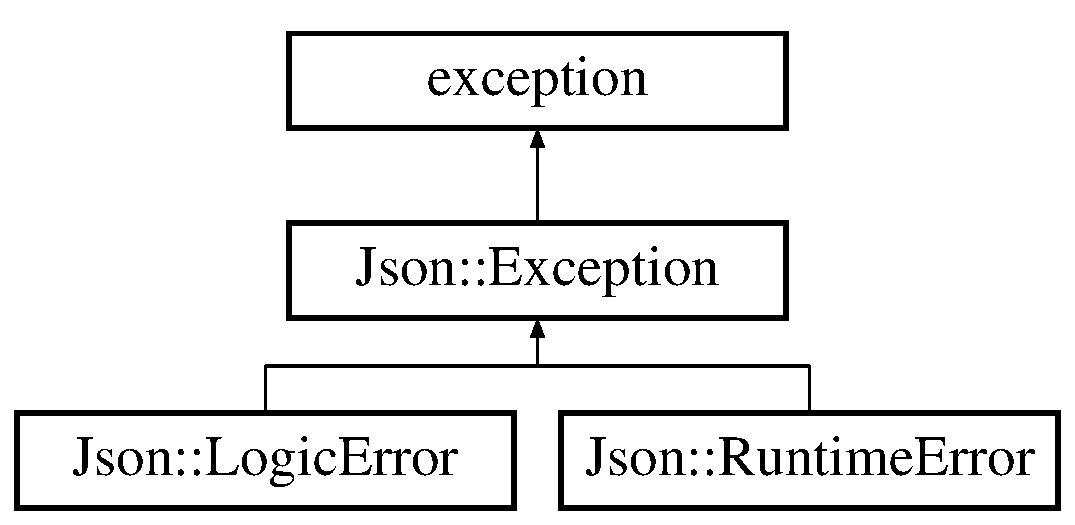
\includegraphics[height=3.000000cm]{class_json_1_1_exception}
\end{center}
\end{figure}
\subsection*{Public Member Functions}
\begin{DoxyCompactItemize}
\item 
\hypertarget{class_json_1_1_exception_a4dd1b9f007bed842e3ef9883d965fe22}{}{\bfseries Exception} (std\+::string const \&msg)\label{class_json_1_1_exception_a4dd1b9f007bed842e3ef9883d965fe22}

\item 
\hypertarget{class_json_1_1_exception_a93032b715e86fc37ad318c60eac4cad7}{}char const $\ast$ {\bfseries what} () const   throw ()\label{class_json_1_1_exception_a93032b715e86fc37ad318c60eac4cad7}

\end{DoxyCompactItemize}
\subsection*{Protected Attributes}
\begin{DoxyCompactItemize}
\item 
\hypertarget{class_json_1_1_exception_a26b7dfcd51256ad4da2742bbd0e14a24}{}std\+::string {\bfseries msg\+\_\+}\label{class_json_1_1_exception_a26b7dfcd51256ad4da2742bbd0e14a24}

\end{DoxyCompactItemize}


\subsection{Detailed Description}
Base class for all exceptions we throw.

We use nothing but these internally. Of course, S\+T\+L can throw others. 

The documentation for this class was generated from the following files\+:\begin{DoxyCompactItemize}
\item 
C\+:/\+Users/\+Mook T/\+Desktop/item/json.\+h\item 
C\+:/\+Users/\+Mook T/\+Desktop/item/jsoncpp.\+cpp\end{DoxyCompactItemize}

\hypertarget{class_json_1_1_char_reader_1_1_factory}{}\section{Json\+:\+:Char\+Reader\+:\+:Factory Class Reference}
\label{class_json_1_1_char_reader_1_1_factory}\index{Json\+::\+Char\+Reader\+::\+Factory@{Json\+::\+Char\+Reader\+::\+Factory}}
Inheritance diagram for Json\+:\+:Char\+Reader\+:\+:Factory\+:\begin{figure}[H]
\begin{center}
\leavevmode
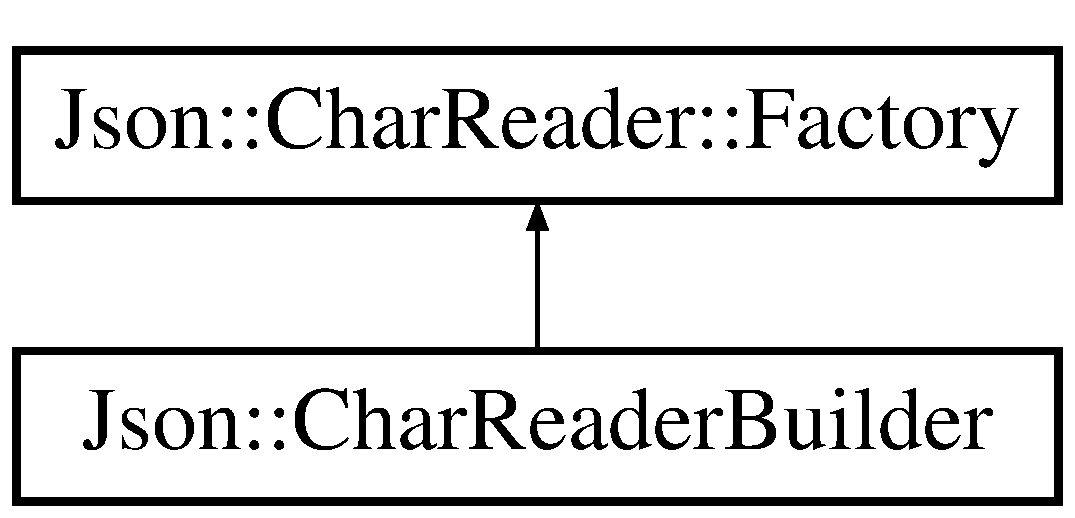
\includegraphics[height=2.000000cm]{class_json_1_1_char_reader_1_1_factory}
\end{center}
\end{figure}
\subsection*{Public Member Functions}
\begin{DoxyCompactItemize}
\item 
virtual \hyperlink{class_json_1_1_char_reader}{Char\+Reader} $\ast$ \hyperlink{class_json_1_1_char_reader_1_1_factory_a497112c51f36a676aeb496c3a91d38d0}{new\+Char\+Reader} () const  =0
\begin{DoxyCompactList}\small\item\em Allocate a \hyperlink{class_json_1_1_char_reader}{Char\+Reader} via operator new(). \end{DoxyCompactList}\end{DoxyCompactItemize}


\subsection{Member Function Documentation}
\hypertarget{class_json_1_1_char_reader_1_1_factory_a497112c51f36a676aeb496c3a91d38d0}{}\index{Json\+::\+Char\+Reader\+::\+Factory@{Json\+::\+Char\+Reader\+::\+Factory}!new\+Char\+Reader@{new\+Char\+Reader}}
\index{new\+Char\+Reader@{new\+Char\+Reader}!Json\+::\+Char\+Reader\+::\+Factory@{Json\+::\+Char\+Reader\+::\+Factory}}
\subsubsection[{new\+Char\+Reader() const  =0}]{\setlength{\rightskip}{0pt plus 5cm}virtual {\bf Char\+Reader}$\ast$ Json\+::\+Char\+Reader\+::\+Factory\+::new\+Char\+Reader (
\begin{DoxyParamCaption}
{}
\end{DoxyParamCaption}
) const\hspace{0.3cm}{\ttfamily [pure virtual]}}\label{class_json_1_1_char_reader_1_1_factory_a497112c51f36a676aeb496c3a91d38d0}


Allocate a \hyperlink{class_json_1_1_char_reader}{Char\+Reader} via operator new(). 


\begin{DoxyExceptions}{Exceptions}
{\em std\+::exception} & if something goes wrong (e.\+g. invalid settings) \\
\hline
\end{DoxyExceptions}


Implemented in \hyperlink{class_json_1_1_char_reader_builder_a3e3c9f4aeb07023ef0c5f6255003078a}{Json\+::\+Char\+Reader\+Builder}.



The documentation for this class was generated from the following file\+:\begin{DoxyCompactItemize}
\item 
C\+:/\+Users/\+Mook T/\+Desktop/item/json.\+h\end{DoxyCompactItemize}

\hypertarget{class_json_1_1_stream_writer_1_1_factory}{}\section{Json\+:\+:Stream\+Writer\+:\+:Factory Class Reference}
\label{class_json_1_1_stream_writer_1_1_factory}\index{Json\+::\+Stream\+Writer\+::\+Factory@{Json\+::\+Stream\+Writer\+::\+Factory}}


A simple abstract factory.  




{\ttfamily \#include $<$json.\+h$>$}

Inheritance diagram for Json\+:\+:Stream\+Writer\+:\+:Factory\+:\begin{figure}[H]
\begin{center}
\leavevmode
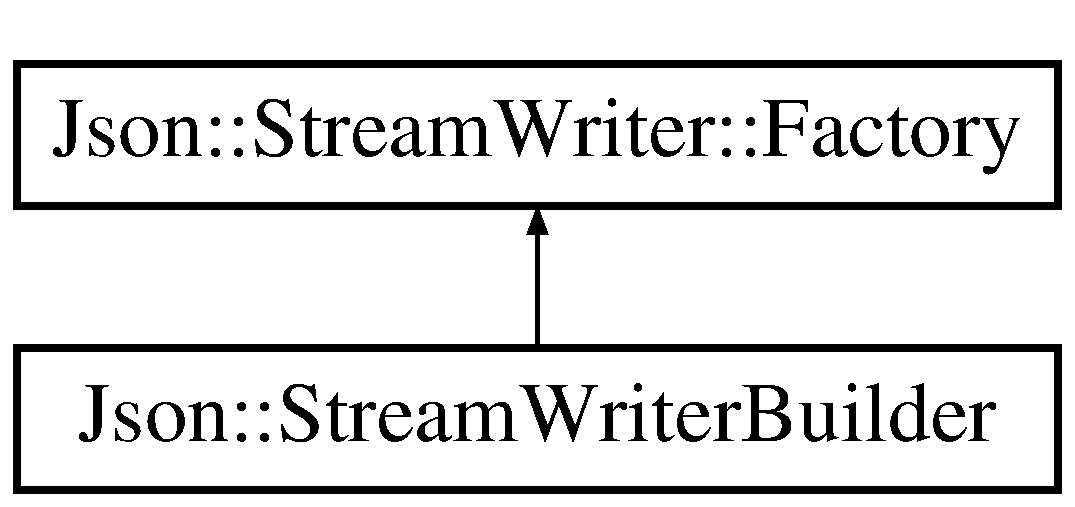
\includegraphics[height=2.000000cm]{class_json_1_1_stream_writer_1_1_factory}
\end{center}
\end{figure}
\subsection*{Public Member Functions}
\begin{DoxyCompactItemize}
\item 
virtual \hyperlink{class_json_1_1_stream_writer}{Stream\+Writer} $\ast$ \hyperlink{class_json_1_1_stream_writer_1_1_factory_a0fca8d713eb8949ca3ebb35e67f23b1a}{new\+Stream\+Writer} () const  =0
\begin{DoxyCompactList}\small\item\em Allocate a \hyperlink{class_json_1_1_char_reader}{Char\+Reader} via operator new(). \end{DoxyCompactList}\end{DoxyCompactItemize}


\subsection{Detailed Description}
A simple abstract factory. 

\subsection{Member Function Documentation}
\hypertarget{class_json_1_1_stream_writer_1_1_factory_a0fca8d713eb8949ca3ebb35e67f23b1a}{}\index{Json\+::\+Stream\+Writer\+::\+Factory@{Json\+::\+Stream\+Writer\+::\+Factory}!new\+Stream\+Writer@{new\+Stream\+Writer}}
\index{new\+Stream\+Writer@{new\+Stream\+Writer}!Json\+::\+Stream\+Writer\+::\+Factory@{Json\+::\+Stream\+Writer\+::\+Factory}}
\subsubsection[{new\+Stream\+Writer() const  =0}]{\setlength{\rightskip}{0pt plus 5cm}virtual {\bf Stream\+Writer}$\ast$ Json\+::\+Stream\+Writer\+::\+Factory\+::new\+Stream\+Writer (
\begin{DoxyParamCaption}
{}
\end{DoxyParamCaption}
) const\hspace{0.3cm}{\ttfamily [pure virtual]}}\label{class_json_1_1_stream_writer_1_1_factory_a0fca8d713eb8949ca3ebb35e67f23b1a}


Allocate a \hyperlink{class_json_1_1_char_reader}{Char\+Reader} via operator new(). 


\begin{DoxyExceptions}{Exceptions}
{\em std\+::exception} & if something goes wrong (e.\+g. invalid settings) \\
\hline
\end{DoxyExceptions}


Implemented in \hyperlink{class_json_1_1_stream_writer_builder_a96c85792f6680835094917ee93915e4b}{Json\+::\+Stream\+Writer\+Builder}.



The documentation for this class was generated from the following files\+:\begin{DoxyCompactItemize}
\item 
C\+:/\+Users/\+Mook T/\+Desktop/item/json.\+h\item 
C\+:/\+Users/\+Mook T/\+Desktop/item/jsoncpp.\+cpp\end{DoxyCompactItemize}

\hypertarget{class_json_1_1_fast_writer}{}\section{Json\+:\+:Fast\+Writer Class Reference}
\label{class_json_1_1_fast_writer}\index{Json\+::\+Fast\+Writer@{Json\+::\+Fast\+Writer}}


Outputs a \hyperlink{class_json_1_1_value}{Value} in \href{http://www.json.org}{\tt J\+S\+O\+N} format without formatting (not human friendly).  




{\ttfamily \#include $<$json.\+h$>$}

Inheritance diagram for Json\+:\+:Fast\+Writer\+:\begin{figure}[H]
\begin{center}
\leavevmode
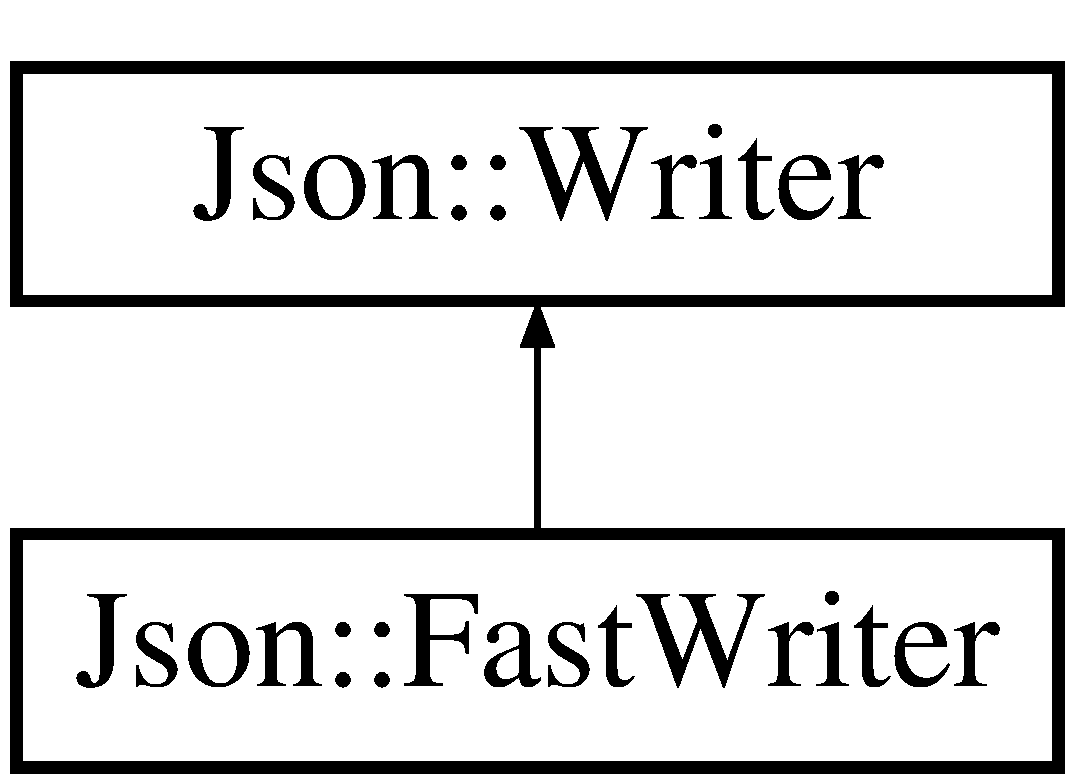
\includegraphics[height=2.000000cm]{class_json_1_1_fast_writer}
\end{center}
\end{figure}
\subsection*{Public Member Functions}
\begin{DoxyCompactItemize}
\item 
\hypertarget{class_json_1_1_fast_writer_a78d98e9f76d33660ad6e6a1abe287d45}{}void {\bfseries enable\+Y\+A\+M\+L\+Compatibility} ()\label{class_json_1_1_fast_writer_a78d98e9f76d33660ad6e6a1abe287d45}

\item 
\hypertarget{class_json_1_1_fast_writer_a6e93d8dce951e408517311026a065b40}{}void \hyperlink{class_json_1_1_fast_writer_a6e93d8dce951e408517311026a065b40}{drop\+Null\+Placeholders} ()\label{class_json_1_1_fast_writer_a6e93d8dce951e408517311026a065b40}

\begin{DoxyCompactList}\small\item\em Drop the \char`\"{}null\char`\"{} string from the writer\textquotesingle{}s output for null\+Values. Strictly speaking, this is not valid J\+S\+O\+N. But when the output is being fed to a browser\textquotesingle{}s Javascript, it makes for smaller output and the browser can handle the output just fine. \end{DoxyCompactList}\item 
\hypertarget{class_json_1_1_fast_writer_af4ee077d365d75941fb2688d97207a55}{}void {\bfseries omit\+Ending\+Line\+Feed} ()\label{class_json_1_1_fast_writer_af4ee077d365d75941fb2688d97207a55}

\item 
\hypertarget{class_json_1_1_fast_writer_aa66218a56447222f91d64db618935a19}{}std\+::string {\bfseries write} (const \hyperlink{class_json_1_1_value}{Value} \&root)\label{class_json_1_1_fast_writer_aa66218a56447222f91d64db618935a19}

\end{DoxyCompactItemize}
\subsection*{Private Member Functions}
\begin{DoxyCompactItemize}
\item 
\hypertarget{class_json_1_1_fast_writer_a2ef4a2ce13a341171f01f414f4fdd765}{}void {\bfseries write\+Value} (const \hyperlink{class_json_1_1_value}{Value} \&value)\label{class_json_1_1_fast_writer_a2ef4a2ce13a341171f01f414f4fdd765}

\end{DoxyCompactItemize}
\subsection*{Private Attributes}
\begin{DoxyCompactItemize}
\item 
\hypertarget{class_json_1_1_fast_writer_afc70d465b79bfc7741ff75294dcefeab}{}std\+::string {\bfseries document\+\_\+}\label{class_json_1_1_fast_writer_afc70d465b79bfc7741ff75294dcefeab}

\item 
\hypertarget{class_json_1_1_fast_writer_a4c4c1911179bf472d24492915b0e489a}{}bool {\bfseries yaml\+Compatiblity\+Enabled\+\_\+}\label{class_json_1_1_fast_writer_a4c4c1911179bf472d24492915b0e489a}

\item 
\hypertarget{class_json_1_1_fast_writer_a97e9d4ff84b59a48756dcc27a71b5904}{}bool {\bfseries drop\+Null\+Placeholders\+\_\+}\label{class_json_1_1_fast_writer_a97e9d4ff84b59a48756dcc27a71b5904}

\item 
\hypertarget{class_json_1_1_fast_writer_abd6e13851db6dcf59d84af68d48d50ac}{}bool {\bfseries omit\+Ending\+Line\+Feed\+\_\+}\label{class_json_1_1_fast_writer_abd6e13851db6dcf59d84af68d48d50ac}

\end{DoxyCompactItemize}


\subsection{Detailed Description}
Outputs a \hyperlink{class_json_1_1_value}{Value} in \href{http://www.json.org}{\tt J\+S\+O\+N} format without formatting (not human friendly). 

The J\+S\+O\+N document is written in a single line. It is not intended for \textquotesingle{}human\textquotesingle{} consumption, but may be usefull to support feature such as R\+P\+C where bandwith is limited. \begin{DoxySeeAlso}{See also}
\hyperlink{class_json_1_1_reader}{Reader}, \hyperlink{class_json_1_1_value}{Value} 
\end{DoxySeeAlso}
\begin{DoxyRefDesc}{Deprecated}
\item[\hyperlink{deprecated__deprecated000008}{Deprecated}]Use \hyperlink{class_json_1_1_stream_writer_builder}{Stream\+Writer\+Builder}. \end{DoxyRefDesc}


The documentation for this class was generated from the following files\+:\begin{DoxyCompactItemize}
\item 
C\+:/\+Users/\+Mook T/\+Desktop/item/json.\+h\item 
C\+:/\+Users/\+Mook T/\+Desktop/item/jsoncpp.\+cpp\end{DoxyCompactItemize}

\hypertarget{class_json_1_1_features}{}\section{Json\+:\+:Features Class Reference}
\label{class_json_1_1_features}\index{Json\+::\+Features@{Json\+::\+Features}}


Configuration passed to reader and writer. This configuration object can be used to force the \hyperlink{class_json_1_1_reader}{Reader} or \hyperlink{class_json_1_1_writer}{Writer} to behave in a standard conforming way.  




{\ttfamily \#include $<$json.\+h$>$}

\subsection*{Public Member Functions}
\begin{DoxyCompactItemize}
\item 
\hypertarget{class_json_1_1_features_ad15a091cb61bb31323299a95970d2644}{}\hyperlink{class_json_1_1_features_ad15a091cb61bb31323299a95970d2644}{Features} ()\label{class_json_1_1_features_ad15a091cb61bb31323299a95970d2644}

\begin{DoxyCompactList}\small\item\em Initialize the configuration like Json\+Config\+::all\+Features;. \end{DoxyCompactList}\end{DoxyCompactItemize}
\subsection*{Static Public Member Functions}
\begin{DoxyCompactItemize}
\item 
static \hyperlink{class_json_1_1_features}{Features} \hyperlink{class_json_1_1_features_a63894da6e2c100b38741fa933f3d33ae}{all} ()
\begin{DoxyCompactList}\small\item\em A configuration that allows all features and assumes all strings are U\+T\+F-\/8. \end{DoxyCompactList}\item 
static \hyperlink{class_json_1_1_features}{Features} \hyperlink{class_json_1_1_features_ae23176c14b2e79e81fb61fb1a8ab58ee}{strict\+Mode} ()
\begin{DoxyCompactList}\small\item\em A configuration that is strictly compatible with the J\+S\+O\+N specification. \end{DoxyCompactList}\end{DoxyCompactItemize}
\subsection*{Public Attributes}
\begin{DoxyCompactItemize}
\item 
\hypertarget{class_json_1_1_features_a33afd389719624b6bdb23950b3c346c9}{}bool \hyperlink{class_json_1_1_features_a33afd389719624b6bdb23950b3c346c9}{allow\+Comments\+\_\+}\label{class_json_1_1_features_a33afd389719624b6bdb23950b3c346c9}

\begin{DoxyCompactList}\small\item\em {\ttfamily true} if comments are allowed. Default\+: {\ttfamily true}. \end{DoxyCompactList}\item 
bool \hyperlink{class_json_1_1_features_a1162c37a1458adc32582b585b552f9c3}{strict\+Root\+\_\+}
\item 
\hypertarget{class_json_1_1_features_a5076aa72c05c7596ac339ede36c97a6a}{}bool \hyperlink{class_json_1_1_features_a5076aa72c05c7596ac339ede36c97a6a}{allow\+Dropped\+Null\+Placeholders\+\_\+}\label{class_json_1_1_features_a5076aa72c05c7596ac339ede36c97a6a}

\begin{DoxyCompactList}\small\item\em {\ttfamily true} if dropped null placeholders are allowed. Default\+: {\ttfamily false}. \end{DoxyCompactList}\item 
\hypertarget{class_json_1_1_features_aff3cb16b79d15d3d761b11a0dd6d4d6b}{}bool \hyperlink{class_json_1_1_features_aff3cb16b79d15d3d761b11a0dd6d4d6b}{allow\+Numeric\+Keys\+\_\+}\label{class_json_1_1_features_aff3cb16b79d15d3d761b11a0dd6d4d6b}

\begin{DoxyCompactList}\small\item\em {\ttfamily true} if numeric object key are allowed. Default\+: {\ttfamily false}. \end{DoxyCompactList}\end{DoxyCompactItemize}


\subsection{Detailed Description}
Configuration passed to reader and writer. This configuration object can be used to force the \hyperlink{class_json_1_1_reader}{Reader} or \hyperlink{class_json_1_1_writer}{Writer} to behave in a standard conforming way. 

\subsection{Member Function Documentation}
\hypertarget{class_json_1_1_features_a63894da6e2c100b38741fa933f3d33ae}{}\index{Json\+::\+Features@{Json\+::\+Features}!all@{all}}
\index{all@{all}!Json\+::\+Features@{Json\+::\+Features}}
\subsubsection[{all()}]{\setlength{\rightskip}{0pt plus 5cm}{\bf Features} Json\+::\+Features\+::all (
\begin{DoxyParamCaption}
{}
\end{DoxyParamCaption}
)\hspace{0.3cm}{\ttfamily [static]}}\label{class_json_1_1_features_a63894da6e2c100b38741fa933f3d33ae}


A configuration that allows all features and assumes all strings are U\+T\+F-\/8. 


\begin{DoxyItemize}
\item C \& C++ comments are allowed
\item Root object can be any J\+S\+O\+N value
\item Assumes \hyperlink{class_json_1_1_value}{Value} strings are encoded in U\+T\+F-\/8 
\end{DoxyItemize}\hypertarget{class_json_1_1_features_ae23176c14b2e79e81fb61fb1a8ab58ee}{}\index{Json\+::\+Features@{Json\+::\+Features}!strict\+Mode@{strict\+Mode}}
\index{strict\+Mode@{strict\+Mode}!Json\+::\+Features@{Json\+::\+Features}}
\subsubsection[{strict\+Mode()}]{\setlength{\rightskip}{0pt plus 5cm}{\bf Features} Json\+::\+Features\+::strict\+Mode (
\begin{DoxyParamCaption}
{}
\end{DoxyParamCaption}
)\hspace{0.3cm}{\ttfamily [static]}}\label{class_json_1_1_features_ae23176c14b2e79e81fb61fb1a8ab58ee}


A configuration that is strictly compatible with the J\+S\+O\+N specification. 


\begin{DoxyItemize}
\item Comments are forbidden.
\item Root object must be either an array or an object value.
\item Assumes \hyperlink{class_json_1_1_value}{Value} strings are encoded in U\+T\+F-\/8 
\end{DoxyItemize}

\subsection{Member Data Documentation}
\hypertarget{class_json_1_1_features_a1162c37a1458adc32582b585b552f9c3}{}\index{Json\+::\+Features@{Json\+::\+Features}!strict\+Root\+\_\+@{strict\+Root\+\_\+}}
\index{strict\+Root\+\_\+@{strict\+Root\+\_\+}!Json\+::\+Features@{Json\+::\+Features}}
\subsubsection[{strict\+Root\+\_\+}]{\setlength{\rightskip}{0pt plus 5cm}bool Json\+::\+Features\+::strict\+Root\+\_\+}\label{class_json_1_1_features_a1162c37a1458adc32582b585b552f9c3}
{\ttfamily true} if root must be either an array or an object value. Default\+: {\ttfamily false}. 

The documentation for this class was generated from the following files\+:\begin{DoxyCompactItemize}
\item 
C\+:/\+Users/\+Mook T/\+Desktop/item/json.\+h\item 
C\+:/\+Users/\+Mook T/\+Desktop/item/jsoncpp.\+cpp\end{DoxyCompactItemize}

\hypertarget{class_item}{}\section{Item Class Reference}
\label{class_item}\index{Item@{Item}}


Abstract \hyperlink{class_item}{Item} Class.  




{\ttfamily \#include $<$Item\+Prototype.\+h$>$}

Inheritance diagram for Item\+:\begin{figure}[H]
\begin{center}
\leavevmode
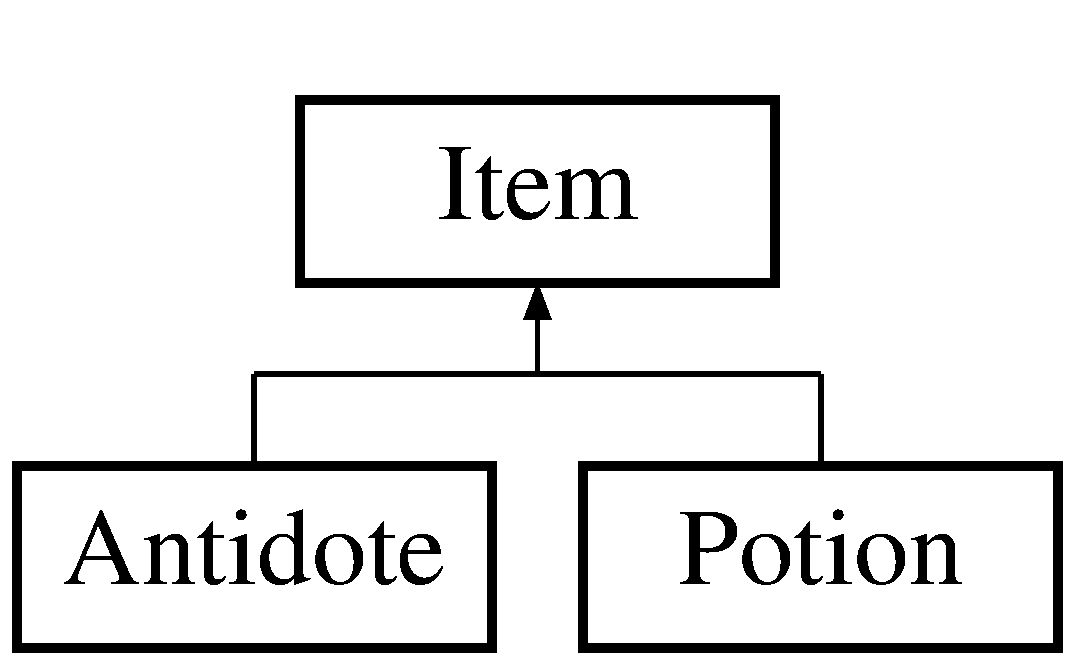
\includegraphics[height=2.000000cm]{class_item}
\end{center}
\end{figure}
\subsection*{Public Member Functions}
\begin{DoxyCompactItemize}
\item 
\hypertarget{class_item_aee86b49539ec0027b06b5c703e386de8}{}virtual \hyperlink{class_item}{Item} $\ast$ \hyperlink{class_item_aee86b49539ec0027b06b5c703e386de8}{clone} (string name)=0\label{class_item_aee86b49539ec0027b06b5c703e386de8}

\begin{DoxyCompactList}\small\item\em Pure virtual clone method. \end{DoxyCompactList}\item 
\hypertarget{class_item_ad3c548eb69bdb99ccbe41bdad8e4eb41}{}void \hyperlink{class_item_ad3c548eb69bdb99ccbe41bdad8e4eb41}{print\+Item} ()\label{class_item_ad3c548eb69bdb99ccbe41bdad8e4eb41}

\begin{DoxyCompactList}\small\item\em Print out statement confirming object has been created. \end{DoxyCompactList}\item 
\hypertarget{class_item_a2aea1cc560205b01eaf5250c21f4fc71}{}string \hyperlink{class_item_a2aea1cc560205b01eaf5250c21f4fc71}{get\+Type} ()\label{class_item_a2aea1cc560205b01eaf5250c21f4fc71}

\begin{DoxyCompactList}\small\item\em Return the type of the object. \end{DoxyCompactList}\item 
\hypertarget{class_item_a63d7f2148b699e539aae354b01559811}{}string \hyperlink{class_item_a63d7f2148b699e539aae354b01559811}{get\+Name} ()\label{class_item_a63d7f2148b699e539aae354b01559811}

\begin{DoxyCompactList}\small\item\em Return the name of the object. \end{DoxyCompactList}\item 
\hypertarget{class_item_a70ce365b03e94a33d4a137dcd9fa2818}{}\hyperlink{class_json_1_1_value}{Json\+::\+Value} \hyperlink{class_item_a70ce365b03e94a33d4a137dcd9fa2818}{to\+Json} () const \label{class_item_a70ce365b03e94a33d4a137dcd9fa2818}

\begin{DoxyCompactList}\small\item\em creating a J\+S\+O\+N object \end{DoxyCompactList}\end{DoxyCompactItemize}
\subsection*{Protected Attributes}
\begin{DoxyCompactItemize}
\item 
\hypertarget{class_item_a1b0c64bfa9407d49b5ad91d6a7372a38}{}string \hyperlink{class_item_a1b0c64bfa9407d49b5ad91d6a7372a38}{item\+Type}\label{class_item_a1b0c64bfa9407d49b5ad91d6a7372a38}

\begin{DoxyCompactList}\small\item\em Store the type of the object. \end{DoxyCompactList}\item 
\hypertarget{class_item_af7a09a8db2072c632d84a992e76408b9}{}string \hyperlink{class_item_af7a09a8db2072c632d84a992e76408b9}{item\+Name}\label{class_item_af7a09a8db2072c632d84a992e76408b9}

\begin{DoxyCompactList}\small\item\em Store the name of the object. \end{DoxyCompactList}\end{DoxyCompactItemize}


\subsection{Detailed Description}
Abstract \hyperlink{class_item}{Item} Class. 

The documentation for this class was generated from the following files\+:\begin{DoxyCompactItemize}
\item 
C\+:/\+Users/\+Mook T/\+Desktop/item/Item\+Prototype.\+h\item 
C\+:/\+Users/\+Mook T/\+Desktop/item/Item\+Prototype.\+cpp\end{DoxyCompactItemize}

\hypertarget{class_item_factory}{}\section{Item\+Factory Class Reference}
\label{class_item_factory}\index{Item\+Factory@{Item\+Factory}}


An \hyperlink{class_item_factory}{Item\+Factory} class.  




{\ttfamily \#include $<$Item\+Prototype.\+h$>$}

\subsection*{Static Public Member Functions}
\begin{DoxyCompactItemize}
\item 
\hypertarget{class_item_factory_a7c6bdc209944c5b0e6a98da6434ef1f7}{}static void \hyperlink{class_item_factory_a7c6bdc209944c5b0e6a98da6434ef1f7}{initialize} ()\label{class_item_factory_a7c6bdc209944c5b0e6a98da6434ef1f7}

\begin{DoxyCompactList}\small\item\em Initialized the prototypes. \end{DoxyCompactList}\item 
\hypertarget{class_item_factory_a47e59f627e5a3ab710138ae6f1c7e6da}{}static \hyperlink{class_item}{Item} $\ast$ \hyperlink{class_item_factory_a47e59f627e5a3ab710138ae6f1c7e6da}{make\+Potion} (string name)\label{class_item_factory_a47e59f627e5a3ab710138ae6f1c7e6da}

\begin{DoxyCompactList}\small\item\em Call the clone() of \hyperlink{class_potion}{Potion} and return the object. \end{DoxyCompactList}\item 
\hypertarget{class_item_factory_a0ece2a36df02fa03f27bf99f145b9019}{}static \hyperlink{class_item}{Item} $\ast$ \hyperlink{class_item_factory_a0ece2a36df02fa03f27bf99f145b9019}{make\+Antidote} (string name)\label{class_item_factory_a0ece2a36df02fa03f27bf99f145b9019}

\begin{DoxyCompactList}\small\item\em Call the clone() of \hyperlink{class_antidote}{Antidote} and return the object. \end{DoxyCompactList}\end{DoxyCompactItemize}
\subsection*{Static Public Attributes}
\begin{DoxyCompactItemize}
\item 
\hypertarget{class_item_factory_a26325ba5225e258360465076f44a8c6c}{}static \hyperlink{class_item}{Item} $\ast$ \hyperlink{class_item_factory_a26325ba5225e258360465076f44a8c6c}{potion} = 0\label{class_item_factory_a26325ba5225e258360465076f44a8c6c}

\begin{DoxyCompactList}\small\item\em A pointer to the \hyperlink{class_potion}{Potion} prototype. \end{DoxyCompactList}\item 
\hypertarget{class_item_factory_aa4b3dbb8ff64d34373907c78a5c6787c}{}static \hyperlink{class_item}{Item} $\ast$ \hyperlink{class_item_factory_aa4b3dbb8ff64d34373907c78a5c6787c}{antidote} = 0\label{class_item_factory_aa4b3dbb8ff64d34373907c78a5c6787c}

\begin{DoxyCompactList}\small\item\em A pointer to the \hyperlink{class_antidote}{Antidote} prototype. \end{DoxyCompactList}\end{DoxyCompactItemize}


\subsection{Detailed Description}
An \hyperlink{class_item_factory}{Item\+Factory} class. 

\hyperlink{class_item_factory}{Item\+Factory} store the prototypes and calls the clone() on that object, and return the object. 

The documentation for this class was generated from the following files\+:\begin{DoxyCompactItemize}
\item 
C\+:/\+Users/\+Mook T/\+Desktop/item/Item\+Prototype.\+h\item 
C\+:/\+Users/\+Mook T/\+Desktop/item/Item\+Prototype.\+cpp\end{DoxyCompactItemize}

\hypertarget{class_json_1_1_logic_error}{}\section{Json\+:\+:Logic\+Error Class Reference}
\label{class_json_1_1_logic_error}\index{Json\+::\+Logic\+Error@{Json\+::\+Logic\+Error}}


{\ttfamily \#include $<$json.\+h$>$}

Inheritance diagram for Json\+:\+:Logic\+Error\+:\begin{figure}[H]
\begin{center}
\leavevmode
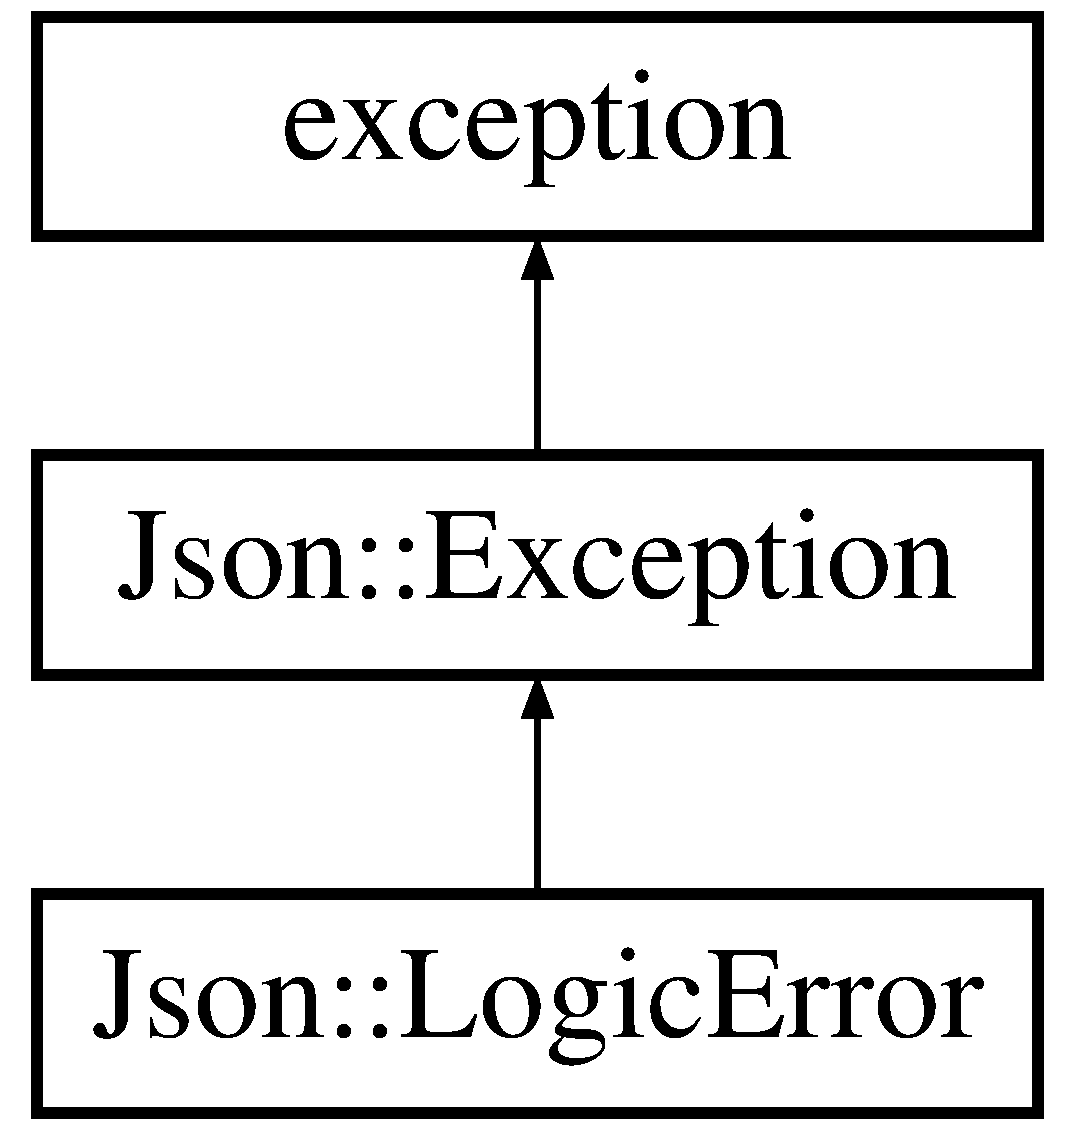
\includegraphics[height=3.000000cm]{class_json_1_1_logic_error}
\end{center}
\end{figure}
\subsection*{Public Member Functions}
\begin{DoxyCompactItemize}
\item 
\hypertarget{class_json_1_1_logic_error_ae8a834c790017a55df74c70b91f23329}{}{\bfseries Logic\+Error} (std\+::string const \&msg)\label{class_json_1_1_logic_error_ae8a834c790017a55df74c70b91f23329}

\end{DoxyCompactItemize}
\subsection*{Additional Inherited Members}


\subsection{Detailed Description}
Exceptions thrown by J\+S\+O\+N\+\_\+\+A\+S\+S\+E\+R\+T/\+J\+S\+O\+N\+\_\+\+F\+A\+I\+L macros.

These are precondition-\/violations (user bugs) and internal errors (our bugs).

\begin{DoxyRemark}{Remarks}
derived from \hyperlink{class_json_1_1_exception}{Json\+::\+Exception} 
\end{DoxyRemark}


The documentation for this class was generated from the following files\+:\begin{DoxyCompactItemize}
\item 
C\+:/\+Users/\+Mook T/\+Desktop/item/json.\+h\item 
C\+:/\+Users/\+Mook T/\+Desktop/item/jsoncpp.\+cpp\end{DoxyCompactItemize}

\hypertarget{class_json_1_1_our_char_reader}{}\section{Json\+:\+:Our\+Char\+Reader Class Reference}
\label{class_json_1_1_our_char_reader}\index{Json\+::\+Our\+Char\+Reader@{Json\+::\+Our\+Char\+Reader}}
Inheritance diagram for Json\+:\+:Our\+Char\+Reader\+:\begin{figure}[H]
\begin{center}
\leavevmode
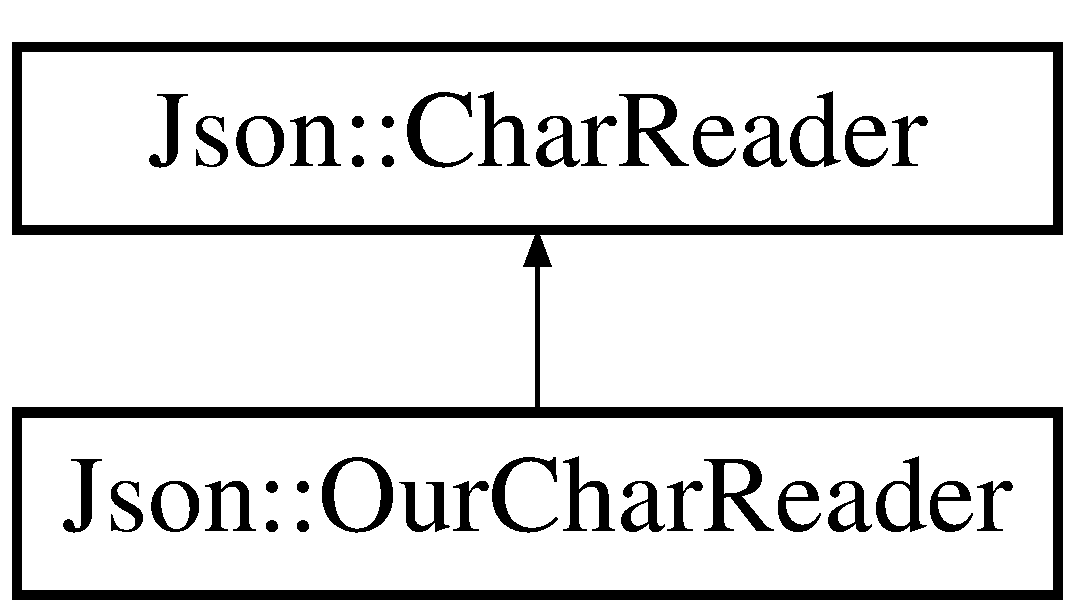
\includegraphics[height=2.000000cm]{class_json_1_1_our_char_reader}
\end{center}
\end{figure}
\subsection*{Public Member Functions}
\begin{DoxyCompactItemize}
\item 
\hypertarget{class_json_1_1_our_char_reader_a5015506620e7ba7bab417756fa1ca9fe}{}{\bfseries Our\+Char\+Reader} (bool collect\+Comments, \hyperlink{class_json_1_1_our_features}{Our\+Features} const \&features)\label{class_json_1_1_our_char_reader_a5015506620e7ba7bab417756fa1ca9fe}

\item 
bool \hyperlink{class_json_1_1_our_char_reader_a268b63f96796d6acea7053fc7c83b05d}{parse} (char const $\ast$begin\+Doc, char const $\ast$end\+Doc, \hyperlink{class_json_1_1_value}{Value} $\ast$root, std\+::string $\ast$errs)
\begin{DoxyCompactList}\small\item\em Read a \hyperlink{class_json_1_1_value}{Value} from a \href{http://www.json.org}{\tt J\+S\+O\+N} document. The document must be a U\+T\+F-\/8 encoded string containing the document to read. \end{DoxyCompactList}\end{DoxyCompactItemize}
\subsection*{Private Attributes}
\begin{DoxyCompactItemize}
\item 
\hypertarget{class_json_1_1_our_char_reader_aa6afd3d0f754cadad0f6d2be38bcfee0}{}bool const {\bfseries collect\+Comments\+\_\+}\label{class_json_1_1_our_char_reader_aa6afd3d0f754cadad0f6d2be38bcfee0}

\item 
\hypertarget{class_json_1_1_our_char_reader_aedd4520b8570654ed7aa0726075ee58d}{}\hyperlink{class_json_1_1_our_reader}{Our\+Reader} {\bfseries reader\+\_\+}\label{class_json_1_1_our_char_reader_aedd4520b8570654ed7aa0726075ee58d}

\end{DoxyCompactItemize}


\subsection{Member Function Documentation}
\hypertarget{class_json_1_1_our_char_reader_a268b63f96796d6acea7053fc7c83b05d}{}\index{Json\+::\+Our\+Char\+Reader@{Json\+::\+Our\+Char\+Reader}!parse@{parse}}
\index{parse@{parse}!Json\+::\+Our\+Char\+Reader@{Json\+::\+Our\+Char\+Reader}}
\subsubsection[{parse(char const $\ast$begin\+Doc, char const $\ast$end\+Doc, Value $\ast$root, std\+::string $\ast$errs)}]{\setlength{\rightskip}{0pt plus 5cm}bool Json\+::\+Our\+Char\+Reader\+::parse (
\begin{DoxyParamCaption}
\item[{char const $\ast$}]{begin\+Doc, }
\item[{char const $\ast$}]{end\+Doc, }
\item[{{\bf Value} $\ast$}]{root, }
\item[{std\+::string $\ast$}]{errs}
\end{DoxyParamCaption}
)\hspace{0.3cm}{\ttfamily [inline]}, {\ttfamily [virtual]}}\label{class_json_1_1_our_char_reader_a268b63f96796d6acea7053fc7c83b05d}


Read a \hyperlink{class_json_1_1_value}{Value} from a \href{http://www.json.org}{\tt J\+S\+O\+N} document. The document must be a U\+T\+F-\/8 encoded string containing the document to read. 


\begin{DoxyParams}{Parameters}
{\em begin\+Doc} & Pointer on the beginning of the U\+T\+F-\/8 encoded string of the document to read. \\
\hline
{\em end\+Doc} & Pointer on the end of the U\+T\+F-\/8 encoded string of the document to read. Must be $>$= begin\+Doc. \\
\hline
{\em root} & \mbox{[}out\mbox{]} Contains the root value of the document if it was successfully parsed. \\
\hline
{\em errs} & \mbox{[}out\mbox{]} Formatted error messages (if not N\+U\+L\+L) a user friendly string that lists errors in the parsed document. \\
\hline
\end{DoxyParams}
\begin{DoxyReturn}{Returns}
{\ttfamily true} if the document was successfully parsed, {\ttfamily false} if an error occurred. 
\end{DoxyReturn}


Implements \hyperlink{class_json_1_1_char_reader_a48e320be8b13bbc0960cc5808cafec98}{Json\+::\+Char\+Reader}.



The documentation for this class was generated from the following file\+:\begin{DoxyCompactItemize}
\item 
C\+:/\+Users/\+Mook T/\+Desktop/item/jsoncpp.\+cpp\end{DoxyCompactItemize}

\hypertarget{class_json_1_1_our_features}{}\section{Json\+:\+:Our\+Features Class Reference}
\label{class_json_1_1_our_features}\index{Json\+::\+Our\+Features@{Json\+::\+Our\+Features}}
\subsection*{Static Public Member Functions}
\begin{DoxyCompactItemize}
\item 
\hypertarget{class_json_1_1_our_features_a0686e1406b6677f496529f9f3fe98d1e}{}static \hyperlink{class_json_1_1_our_features}{Our\+Features} {\bfseries all} ()\label{class_json_1_1_our_features_a0686e1406b6677f496529f9f3fe98d1e}

\end{DoxyCompactItemize}
\subsection*{Public Attributes}
\begin{DoxyCompactItemize}
\item 
\hypertarget{class_json_1_1_our_features_ac71bb7ba7363d3b05ed76602b036ce33}{}bool {\bfseries allow\+Comments\+\_\+}\label{class_json_1_1_our_features_ac71bb7ba7363d3b05ed76602b036ce33}

\item 
\hypertarget{class_json_1_1_our_features_a2095f66a776c0a4ae6cc931a0c94242e}{}bool {\bfseries strict\+Root\+\_\+}\label{class_json_1_1_our_features_a2095f66a776c0a4ae6cc931a0c94242e}

\item 
\hypertarget{class_json_1_1_our_features_a13963bc44bf948eec1968f7ff8e8f5f1}{}bool {\bfseries allow\+Dropped\+Null\+Placeholders\+\_\+}\label{class_json_1_1_our_features_a13963bc44bf948eec1968f7ff8e8f5f1}

\item 
\hypertarget{class_json_1_1_our_features_af6973fc7e774ce2d634ba99442aeb91a}{}bool {\bfseries allow\+Numeric\+Keys\+\_\+}\label{class_json_1_1_our_features_af6973fc7e774ce2d634ba99442aeb91a}

\item 
\hypertarget{class_json_1_1_our_features_abbd6c196d7a22e2a360a59887eda4610}{}bool {\bfseries allow\+Single\+Quotes\+\_\+}\label{class_json_1_1_our_features_abbd6c196d7a22e2a360a59887eda4610}

\item 
\hypertarget{class_json_1_1_our_features_ae8ad25b90706c78f1a8fe929191ac61b}{}bool {\bfseries fail\+If\+Extra\+\_\+}\label{class_json_1_1_our_features_ae8ad25b90706c78f1a8fe929191ac61b}

\item 
\hypertarget{class_json_1_1_our_features_a39b8e0b86b1c24a45e800c023bb715aa}{}bool {\bfseries reject\+Dup\+Keys\+\_\+}\label{class_json_1_1_our_features_a39b8e0b86b1c24a45e800c023bb715aa}

\item 
\hypertarget{class_json_1_1_our_features_af760f91cc2a7af37e44f78fb466061bb}{}bool {\bfseries allow\+Special\+Floats\+\_\+}\label{class_json_1_1_our_features_af760f91cc2a7af37e44f78fb466061bb}

\item 
\hypertarget{class_json_1_1_our_features_a9a786713902d14be6d57a08cc03ccfff}{}int {\bfseries stack\+Limit\+\_\+}\label{class_json_1_1_our_features_a9a786713902d14be6d57a08cc03ccfff}

\end{DoxyCompactItemize}


The documentation for this class was generated from the following file\+:\begin{DoxyCompactItemize}
\item 
C\+:/\+Users/\+Mook T/\+Desktop/item/jsoncpp.\+cpp\end{DoxyCompactItemize}

\hypertarget{class_json_1_1_our_reader}{}\section{Json\+:\+:Our\+Reader Class Reference}
\label{class_json_1_1_our_reader}\index{Json\+::\+Our\+Reader@{Json\+::\+Our\+Reader}}
\subsection*{Classes}
\begin{DoxyCompactItemize}
\item 
class \hyperlink{class_json_1_1_our_reader_1_1_error_info}{Error\+Info}
\item 
struct \hyperlink{struct_json_1_1_our_reader_1_1_structured_error}{Structured\+Error}
\item 
class \hyperlink{class_json_1_1_our_reader_1_1_token}{Token}
\end{DoxyCompactItemize}
\subsection*{Public Types}
\begin{DoxyCompactItemize}
\item 
\hypertarget{class_json_1_1_our_reader_a0cd0bab4caa66594ab843ccd5f9dc239}{}typedef char {\bfseries Char}\label{class_json_1_1_our_reader_a0cd0bab4caa66594ab843ccd5f9dc239}

\item 
\hypertarget{class_json_1_1_our_reader_a1bdc7bbc52ba87cae6b19746f2ee0189}{}typedef const Char $\ast$ {\bfseries Location}\label{class_json_1_1_our_reader_a1bdc7bbc52ba87cae6b19746f2ee0189}

\end{DoxyCompactItemize}
\subsection*{Public Member Functions}
\begin{DoxyCompactItemize}
\item 
\hypertarget{class_json_1_1_our_reader_a48a850914b9c8d7781be172930c478e5}{}{\bfseries Our\+Reader} (\hyperlink{class_json_1_1_our_features}{Our\+Features} const \&features)\label{class_json_1_1_our_reader_a48a850914b9c8d7781be172930c478e5}

\item 
\hypertarget{class_json_1_1_our_reader_aba4f8749aab7f02ec17f107e392caf80}{}bool {\bfseries parse} (const char $\ast$begin\+Doc, const char $\ast$end\+Doc, \hyperlink{class_json_1_1_value}{Value} \&root, bool collect\+Comments=true)\label{class_json_1_1_our_reader_aba4f8749aab7f02ec17f107e392caf80}

\item 
\hypertarget{class_json_1_1_our_reader_ae9cbb7dbd9c6c96be37432e8dfa1afcb}{}std\+::string {\bfseries get\+Formatted\+Error\+Messages} () const \label{class_json_1_1_our_reader_ae9cbb7dbd9c6c96be37432e8dfa1afcb}

\item 
\hypertarget{class_json_1_1_our_reader_a02ef7871af3706754a233c36e6d489e9}{}std\+::vector$<$ \hyperlink{struct_json_1_1_our_reader_1_1_structured_error}{Structured\+Error} $>$ {\bfseries get\+Structured\+Errors} () const \label{class_json_1_1_our_reader_a02ef7871af3706754a233c36e6d489e9}

\item 
\hypertarget{class_json_1_1_our_reader_aef7aa4ca22ffaa38c401b16951d20e1e}{}bool {\bfseries push\+Error} (const \hyperlink{class_json_1_1_value}{Value} \&value, const std\+::string \&message)\label{class_json_1_1_our_reader_aef7aa4ca22ffaa38c401b16951d20e1e}

\item 
\hypertarget{class_json_1_1_our_reader_ad43315cbb0d6804e3b7177e84a1ec53d}{}bool {\bfseries push\+Error} (const \hyperlink{class_json_1_1_value}{Value} \&value, const std\+::string \&message, const \hyperlink{class_json_1_1_value}{Value} \&extra)\label{class_json_1_1_our_reader_ad43315cbb0d6804e3b7177e84a1ec53d}

\item 
\hypertarget{class_json_1_1_our_reader_a048346238d703ad9aed06beb686e6102}{}bool {\bfseries good} () const \label{class_json_1_1_our_reader_a048346238d703ad9aed06beb686e6102}

\end{DoxyCompactItemize}
\subsection*{Private Types}
\begin{DoxyCompactItemize}
\item 
\hypertarget{class_json_1_1_our_reader_a15116f7276ddf1e7a2cc3cbefa884dcc}{}enum {\bfseries Token\+Type} \{ \\*
{\bfseries token\+End\+Of\+Stream} = 0, 
{\bfseries token\+Object\+Begin}, 
{\bfseries token\+Object\+End}, 
{\bfseries token\+Array\+Begin}, 
\\*
{\bfseries token\+Array\+End}, 
{\bfseries token\+String}, 
{\bfseries token\+Number}, 
{\bfseries token\+True}, 
\\*
{\bfseries token\+False}, 
{\bfseries token\+Null}, 
{\bfseries token\+Na\+N}, 
{\bfseries token\+Pos\+Inf}, 
\\*
{\bfseries token\+Neg\+Inf}, 
{\bfseries token\+Array\+Separator}, 
{\bfseries token\+Member\+Separator}, 
{\bfseries token\+Comment}, 
\\*
{\bfseries token\+Error}
 \}\label{class_json_1_1_our_reader_a15116f7276ddf1e7a2cc3cbefa884dcc}

\item 
\hypertarget{class_json_1_1_our_reader_a8cc69593ef7303e58e99bb5dbb767562}{}typedef std\+::deque$<$ \hyperlink{class_json_1_1_our_reader_1_1_error_info}{Error\+Info} $>$ {\bfseries Errors}\label{class_json_1_1_our_reader_a8cc69593ef7303e58e99bb5dbb767562}

\item 
\hypertarget{class_json_1_1_our_reader_a8480a5ef159cee3a090f96358414d8d3}{}typedef std\+::stack$<$ \hyperlink{class_json_1_1_value}{Value} $\ast$ $>$ {\bfseries Nodes}\label{class_json_1_1_our_reader_a8480a5ef159cee3a090f96358414d8d3}

\end{DoxyCompactItemize}
\subsection*{Private Member Functions}
\begin{DoxyCompactItemize}
\item 
\hypertarget{class_json_1_1_our_reader_aee013005522c0d34d2e14962851487ac}{}{\bfseries Our\+Reader} (\hyperlink{class_json_1_1_our_reader}{Our\+Reader} const \&)\label{class_json_1_1_our_reader_aee013005522c0d34d2e14962851487ac}

\item 
\hypertarget{class_json_1_1_our_reader_ad418de7c47bd3d0510888e22110b796e}{}void {\bfseries operator=} (\hyperlink{class_json_1_1_our_reader}{Our\+Reader} const \&)\label{class_json_1_1_our_reader_ad418de7c47bd3d0510888e22110b796e}

\item 
\hypertarget{class_json_1_1_our_reader_a0d1e66da47fe2e85f5033c59326dfdc3}{}bool {\bfseries read\+Token} (\hyperlink{class_json_1_1_our_reader_1_1_token}{Token} \&token)\label{class_json_1_1_our_reader_a0d1e66da47fe2e85f5033c59326dfdc3}

\item 
\hypertarget{class_json_1_1_our_reader_a6fbc6d58a4505e5ccadf330b57b17ca5}{}void {\bfseries skip\+Spaces} ()\label{class_json_1_1_our_reader_a6fbc6d58a4505e5ccadf330b57b17ca5}

\item 
\hypertarget{class_json_1_1_our_reader_a4a03f1b266def9b47c4fef35386557fb}{}bool {\bfseries match} (Location pattern, int pattern\+Length)\label{class_json_1_1_our_reader_a4a03f1b266def9b47c4fef35386557fb}

\item 
\hypertarget{class_json_1_1_our_reader_a90f6bb9e55b2bc3d6c1880809495c222}{}bool {\bfseries read\+Comment} ()\label{class_json_1_1_our_reader_a90f6bb9e55b2bc3d6c1880809495c222}

\item 
\hypertarget{class_json_1_1_our_reader_aba784b125baa1b62387e767b791f2f89}{}bool {\bfseries read\+C\+Style\+Comment} ()\label{class_json_1_1_our_reader_aba784b125baa1b62387e767b791f2f89}

\item 
\hypertarget{class_json_1_1_our_reader_ae3de80671f0f997053e1c1c8a47a45c5}{}bool {\bfseries read\+Cpp\+Style\+Comment} ()\label{class_json_1_1_our_reader_ae3de80671f0f997053e1c1c8a47a45c5}

\item 
\hypertarget{class_json_1_1_our_reader_a5d39b12671499ec5975f3bbc84b7d438}{}bool {\bfseries read\+String} ()\label{class_json_1_1_our_reader_a5d39b12671499ec5975f3bbc84b7d438}

\item 
\hypertarget{class_json_1_1_our_reader_ac78592defdc333faf56c6d0908758da3}{}bool {\bfseries read\+String\+Single\+Quote} ()\label{class_json_1_1_our_reader_ac78592defdc333faf56c6d0908758da3}

\item 
\hypertarget{class_json_1_1_our_reader_aefcb9a78cc45870ccac2db2a66c8ec50}{}bool {\bfseries read\+Number} (bool check\+Inf)\label{class_json_1_1_our_reader_aefcb9a78cc45870ccac2db2a66c8ec50}

\item 
\hypertarget{class_json_1_1_our_reader_a1765d9670d191c89a57a22ea5591d35f}{}bool {\bfseries read\+Value} ()\label{class_json_1_1_our_reader_a1765d9670d191c89a57a22ea5591d35f}

\item 
\hypertarget{class_json_1_1_our_reader_aea198f8101dba55099f4d8121a993530}{}bool {\bfseries read\+Object} (\hyperlink{class_json_1_1_our_reader_1_1_token}{Token} \&token)\label{class_json_1_1_our_reader_aea198f8101dba55099f4d8121a993530}

\item 
\hypertarget{class_json_1_1_our_reader_a0b9f58faf4212c6ecb5d8e2a1ac10257}{}bool {\bfseries read\+Array} (\hyperlink{class_json_1_1_our_reader_1_1_token}{Token} \&token)\label{class_json_1_1_our_reader_a0b9f58faf4212c6ecb5d8e2a1ac10257}

\item 
\hypertarget{class_json_1_1_our_reader_a272d271290933a89abfd5096dd69c9e9}{}bool {\bfseries decode\+Number} (\hyperlink{class_json_1_1_our_reader_1_1_token}{Token} \&token)\label{class_json_1_1_our_reader_a272d271290933a89abfd5096dd69c9e9}

\item 
\hypertarget{class_json_1_1_our_reader_a712270d53a2f023c2f406ac813548340}{}bool {\bfseries decode\+Number} (\hyperlink{class_json_1_1_our_reader_1_1_token}{Token} \&token, \hyperlink{class_json_1_1_value}{Value} \&decoded)\label{class_json_1_1_our_reader_a712270d53a2f023c2f406ac813548340}

\item 
\hypertarget{class_json_1_1_our_reader_a34e31d8b8399b7ad493359702b6de6c9}{}bool {\bfseries decode\+String} (\hyperlink{class_json_1_1_our_reader_1_1_token}{Token} \&token)\label{class_json_1_1_our_reader_a34e31d8b8399b7ad493359702b6de6c9}

\item 
\hypertarget{class_json_1_1_our_reader_a44b589a85f02f0e2de1b4ad6916be0c5}{}bool {\bfseries decode\+String} (\hyperlink{class_json_1_1_our_reader_1_1_token}{Token} \&token, std\+::string \&decoded)\label{class_json_1_1_our_reader_a44b589a85f02f0e2de1b4ad6916be0c5}

\item 
\hypertarget{class_json_1_1_our_reader_a1d1c3b44f6720a0e7c39b5ae8de3981c}{}bool {\bfseries decode\+Double} (\hyperlink{class_json_1_1_our_reader_1_1_token}{Token} \&token)\label{class_json_1_1_our_reader_a1d1c3b44f6720a0e7c39b5ae8de3981c}

\item 
\hypertarget{class_json_1_1_our_reader_aa5c15a8cd32754f07430dedba3d1308e}{}bool {\bfseries decode\+Double} (\hyperlink{class_json_1_1_our_reader_1_1_token}{Token} \&token, \hyperlink{class_json_1_1_value}{Value} \&decoded)\label{class_json_1_1_our_reader_aa5c15a8cd32754f07430dedba3d1308e}

\item 
\hypertarget{class_json_1_1_our_reader_ac1bf03c161ece082e48da450c50f528d}{}bool {\bfseries decode\+Unicode\+Code\+Point} (\hyperlink{class_json_1_1_our_reader_1_1_token}{Token} \&token, Location \&current, Location end, unsigned int \&unicode)\label{class_json_1_1_our_reader_ac1bf03c161ece082e48da450c50f528d}

\item 
\hypertarget{class_json_1_1_our_reader_adb39be814cc6076b91a0919bdd5b24b0}{}bool {\bfseries decode\+Unicode\+Escape\+Sequence} (\hyperlink{class_json_1_1_our_reader_1_1_token}{Token} \&token, Location \&current, Location end, unsigned int \&unicode)\label{class_json_1_1_our_reader_adb39be814cc6076b91a0919bdd5b24b0}

\item 
\hypertarget{class_json_1_1_our_reader_a5a48b71c1c16fa671814c8338e452bc0}{}bool {\bfseries add\+Error} (const std\+::string \&message, \hyperlink{class_json_1_1_our_reader_1_1_token}{Token} \&token, Location extra=0)\label{class_json_1_1_our_reader_a5a48b71c1c16fa671814c8338e452bc0}

\item 
\hypertarget{class_json_1_1_our_reader_a035651f0700a76a815e5f904c63ebb1c}{}bool {\bfseries recover\+From\+Error} (Token\+Type skip\+Until\+Token)\label{class_json_1_1_our_reader_a035651f0700a76a815e5f904c63ebb1c}

\item 
\hypertarget{class_json_1_1_our_reader_ae68a7047acd692be8077e259d524c6d9}{}bool {\bfseries add\+Error\+And\+Recover} (const std\+::string \&message, \hyperlink{class_json_1_1_our_reader_1_1_token}{Token} \&token, Token\+Type skip\+Until\+Token)\label{class_json_1_1_our_reader_ae68a7047acd692be8077e259d524c6d9}

\item 
\hypertarget{class_json_1_1_our_reader_ad48bdaf5b686706f003e792fdbcbf102}{}void {\bfseries skip\+Until\+Space} ()\label{class_json_1_1_our_reader_ad48bdaf5b686706f003e792fdbcbf102}

\item 
\hypertarget{class_json_1_1_our_reader_a2acd5b1d53e7d7e17c21ff8e96edc09d}{}\hyperlink{class_json_1_1_value}{Value} \& {\bfseries current\+Value} ()\label{class_json_1_1_our_reader_a2acd5b1d53e7d7e17c21ff8e96edc09d}

\item 
\hypertarget{class_json_1_1_our_reader_a298285d035fdbc554caae09d9f0a5859}{}Char {\bfseries get\+Next\+Char} ()\label{class_json_1_1_our_reader_a298285d035fdbc554caae09d9f0a5859}

\item 
\hypertarget{class_json_1_1_our_reader_a9f47ad324225df1e68bda7dc451845c9}{}void {\bfseries get\+Location\+Line\+And\+Column} (Location location, int \&line, int \&column) const \label{class_json_1_1_our_reader_a9f47ad324225df1e68bda7dc451845c9}

\item 
\hypertarget{class_json_1_1_our_reader_a579a7d2e493f63c4b122103844e3cedd}{}std\+::string {\bfseries get\+Location\+Line\+And\+Column} (Location location) const \label{class_json_1_1_our_reader_a579a7d2e493f63c4b122103844e3cedd}

\item 
\hypertarget{class_json_1_1_our_reader_ad7318c37469a9106069a236fb4b10e1f}{}void {\bfseries add\+Comment} (Location begin, Location end, \hyperlink{namespace_json_a4fc417c23905b2ae9e2c47d197a45351}{Comment\+Placement} placement)\label{class_json_1_1_our_reader_ad7318c37469a9106069a236fb4b10e1f}

\item 
\hypertarget{class_json_1_1_our_reader_a856dea44d92578c276856d7a65a4ebdc}{}void {\bfseries skip\+Comment\+Tokens} (\hyperlink{class_json_1_1_our_reader_1_1_token}{Token} \&token)\label{class_json_1_1_our_reader_a856dea44d92578c276856d7a65a4ebdc}

\end{DoxyCompactItemize}
\subsection*{Private Attributes}
\begin{DoxyCompactItemize}
\item 
\hypertarget{class_json_1_1_our_reader_a19cc4e8c5d17ee6822f752e9a36f4ce3}{}Nodes {\bfseries nodes\+\_\+}\label{class_json_1_1_our_reader_a19cc4e8c5d17ee6822f752e9a36f4ce3}

\item 
\hypertarget{class_json_1_1_our_reader_afb76b68ba1ab68fe09cf2838e3d4898d}{}Errors {\bfseries errors\+\_\+}\label{class_json_1_1_our_reader_afb76b68ba1ab68fe09cf2838e3d4898d}

\item 
\hypertarget{class_json_1_1_our_reader_aeb9b8bb85fa8a4dd72e546bb3104c597}{}std\+::string {\bfseries document\+\_\+}\label{class_json_1_1_our_reader_aeb9b8bb85fa8a4dd72e546bb3104c597}

\item 
\hypertarget{class_json_1_1_our_reader_a9bda9d72335d52cd06e65f9eca3f70f5}{}Location {\bfseries begin\+\_\+}\label{class_json_1_1_our_reader_a9bda9d72335d52cd06e65f9eca3f70f5}

\item 
\hypertarget{class_json_1_1_our_reader_ab1f69b0260c27a0d2d65dc56e42c8f9d}{}Location {\bfseries end\+\_\+}\label{class_json_1_1_our_reader_ab1f69b0260c27a0d2d65dc56e42c8f9d}

\item 
\hypertarget{class_json_1_1_our_reader_a5211fbbba94be80a22dd2317c621efcc}{}Location {\bfseries current\+\_\+}\label{class_json_1_1_our_reader_a5211fbbba94be80a22dd2317c621efcc}

\item 
\hypertarget{class_json_1_1_our_reader_a101eadc45e01c60628b53f0db3d13482}{}Location {\bfseries last\+Value\+End\+\_\+}\label{class_json_1_1_our_reader_a101eadc45e01c60628b53f0db3d13482}

\item 
\hypertarget{class_json_1_1_our_reader_a9f994b6a2227c5d96e6ed6cbc74ed251}{}\hyperlink{class_json_1_1_value}{Value} $\ast$ {\bfseries last\+Value\+\_\+}\label{class_json_1_1_our_reader_a9f994b6a2227c5d96e6ed6cbc74ed251}

\item 
\hypertarget{class_json_1_1_our_reader_a2e8fd643b2e85155f5292db8fc9c6084}{}std\+::string {\bfseries comments\+Before\+\_\+}\label{class_json_1_1_our_reader_a2e8fd643b2e85155f5292db8fc9c6084}

\item 
\hypertarget{class_json_1_1_our_reader_aaa91c93bc064c7086248ea01eddcf51a}{}int {\bfseries stack\+Depth\+\_\+}\label{class_json_1_1_our_reader_aaa91c93bc064c7086248ea01eddcf51a}

\item 
\hypertarget{class_json_1_1_our_reader_a2714302d5cc54ca2ce4118ea51c0397a}{}\hyperlink{class_json_1_1_our_features}{Our\+Features} const {\bfseries features\+\_\+}\label{class_json_1_1_our_reader_a2714302d5cc54ca2ce4118ea51c0397a}

\item 
\hypertarget{class_json_1_1_our_reader_a259f6ac988da2894bcafc670e42f73ad}{}bool {\bfseries collect\+Comments\+\_\+}\label{class_json_1_1_our_reader_a259f6ac988da2894bcafc670e42f73ad}

\end{DoxyCompactItemize}


The documentation for this class was generated from the following file\+:\begin{DoxyCompactItemize}
\item 
C\+:/\+Users/\+Mook T/\+Desktop/item/jsoncpp.\+cpp\end{DoxyCompactItemize}

\hypertarget{class_json_1_1_path}{}\section{Json\+:\+:Path Class Reference}
\label{class_json_1_1_path}\index{Json\+::\+Path@{Json\+::\+Path}}


Experimental and untested\+: represents a \char`\"{}path\char`\"{} to access a node.  




{\ttfamily \#include $<$json.\+h$>$}

\subsection*{Public Member Functions}
\begin{DoxyCompactItemize}
\item 
\hypertarget{class_json_1_1_path_aaa37a99650e770d0cd680bf53585ec99}{}{\bfseries Path} (const std\+::string \&path, const \hyperlink{class_json_1_1_path_argument}{Path\+Argument} \&a1=\hyperlink{class_json_1_1_path_argument}{Path\+Argument}(), const \hyperlink{class_json_1_1_path_argument}{Path\+Argument} \&a2=\hyperlink{class_json_1_1_path_argument}{Path\+Argument}(), const \hyperlink{class_json_1_1_path_argument}{Path\+Argument} \&a3=\hyperlink{class_json_1_1_path_argument}{Path\+Argument}(), const \hyperlink{class_json_1_1_path_argument}{Path\+Argument} \&a4=\hyperlink{class_json_1_1_path_argument}{Path\+Argument}(), const \hyperlink{class_json_1_1_path_argument}{Path\+Argument} \&a5=\hyperlink{class_json_1_1_path_argument}{Path\+Argument}())\label{class_json_1_1_path_aaa37a99650e770d0cd680bf53585ec99}

\item 
\hypertarget{class_json_1_1_path_ae1d05fa985a6ee3c57f2b8ed186b5982}{}const \hyperlink{class_json_1_1_value}{Value} \& {\bfseries resolve} (const \hyperlink{class_json_1_1_value}{Value} \&root) const \label{class_json_1_1_path_ae1d05fa985a6ee3c57f2b8ed186b5982}

\item 
\hypertarget{class_json_1_1_path_a33d1749770a4cf74e9a3de419bc7febe}{}\hyperlink{class_json_1_1_value}{Value} {\bfseries resolve} (const \hyperlink{class_json_1_1_value}{Value} \&root, const \hyperlink{class_json_1_1_value}{Value} \&default\+Value) const \label{class_json_1_1_path_a33d1749770a4cf74e9a3de419bc7febe}

\item 
\hyperlink{class_json_1_1_value}{Value} \& \hyperlink{class_json_1_1_path_a5289901fc58ad1fdca1de7fb5a0b620c}{make} (\hyperlink{class_json_1_1_value}{Value} \&root) const 
\end{DoxyCompactItemize}
\subsection*{Private Types}
\begin{DoxyCompactItemize}
\item 
\hypertarget{class_json_1_1_path_ab29d7b2fc896c7d3c5ed4609af3a3f23}{}typedef std\+::vector$<$ const \hyperlink{class_json_1_1_path_argument}{Path\+Argument} $\ast$ $>$ {\bfseries In\+Args}\label{class_json_1_1_path_ab29d7b2fc896c7d3c5ed4609af3a3f23}

\item 
\hypertarget{class_json_1_1_path_a27d96232d034d7a78286468676f9cb3e}{}typedef std\+::vector$<$ \hyperlink{class_json_1_1_path_argument}{Path\+Argument} $>$ {\bfseries Args}\label{class_json_1_1_path_a27d96232d034d7a78286468676f9cb3e}

\end{DoxyCompactItemize}
\subsection*{Private Member Functions}
\begin{DoxyCompactItemize}
\item 
\hypertarget{class_json_1_1_path_a874e5339f8059ebeef049721f8897277}{}void {\bfseries make\+Path} (const std\+::string \&path, const In\+Args \&in)\label{class_json_1_1_path_a874e5339f8059ebeef049721f8897277}

\item 
\hypertarget{class_json_1_1_path_af4d2ab3a6f09b69bab3d3e9fcdf13328}{}void {\bfseries add\+Path\+In\+Arg} (const std\+::string \&path, const In\+Args \&in, In\+Args\+::const\+\_\+iterator \&it\+In\+Arg, Path\+Argument\+::\+Kind kind)\label{class_json_1_1_path_af4d2ab3a6f09b69bab3d3e9fcdf13328}

\item 
\hypertarget{class_json_1_1_path_a3729e6d3682338b2cfad2c10d4746f53}{}void {\bfseries invalid\+Path} (const std\+::string \&path, int location)\label{class_json_1_1_path_a3729e6d3682338b2cfad2c10d4746f53}

\end{DoxyCompactItemize}
\subsection*{Private Attributes}
\begin{DoxyCompactItemize}
\item 
\hypertarget{class_json_1_1_path_af33d0de7ee9f99d3e361bdf504dc2bc7}{}Args {\bfseries args\+\_\+}\label{class_json_1_1_path_af33d0de7ee9f99d3e361bdf504dc2bc7}

\end{DoxyCompactItemize}


\subsection{Detailed Description}
Experimental and untested\+: represents a \char`\"{}path\char`\"{} to access a node. 

Syntax\+:
\begin{DoxyItemize}
\item \char`\"{}.\char`\"{} =$>$ root node
\item \char`\"{}.\mbox{[}n\mbox{]}\char`\"{} =$>$ elements at index \textquotesingle{}n\textquotesingle{} of root node (an array value)
\item \char`\"{}.\+name\char`\"{} =$>$ member named \textquotesingle{}name\textquotesingle{} of root node (an object value)
\item \char`\"{}.\+name1.\+name2.\+name3\char`\"{}
\item \char`\"{}.\mbox{[}0\mbox{]}\mbox{[}1\mbox{]}\mbox{[}2\mbox{]}.\+name1\mbox{[}3\mbox{]}\char`\"{}
\item \char`\"{}.\%\char`\"{} =$>$ member name is provided as parameter
\item \char`\"{}.\mbox{[}\%\mbox{]}\char`\"{} =$>$ index is provied as parameter 
\end{DoxyItemize}

\subsection{Member Function Documentation}
\hypertarget{class_json_1_1_path_a5289901fc58ad1fdca1de7fb5a0b620c}{}\index{Json\+::\+Path@{Json\+::\+Path}!make@{make}}
\index{make@{make}!Json\+::\+Path@{Json\+::\+Path}}
\subsubsection[{make(\+Value \&root) const }]{\setlength{\rightskip}{0pt plus 5cm}{\bf Value} \& Json\+::\+Path\+::make (
\begin{DoxyParamCaption}
\item[{{\bf Value} \&}]{root}
\end{DoxyParamCaption}
) const}\label{class_json_1_1_path_a5289901fc58ad1fdca1de7fb5a0b620c}
Creates the \char`\"{}path\char`\"{} to access the specified node and returns a reference on the node. 

The documentation for this class was generated from the following files\+:\begin{DoxyCompactItemize}
\item 
C\+:/\+Users/\+Mook T/\+Desktop/item/json.\+h\item 
C\+:/\+Users/\+Mook T/\+Desktop/item/jsoncpp.\+cpp\end{DoxyCompactItemize}

\hypertarget{class_json_1_1_path_argument}{}\section{Json\+:\+:Path\+Argument Class Reference}
\label{class_json_1_1_path_argument}\index{Json\+::\+Path\+Argument@{Json\+::\+Path\+Argument}}


Experimental and untested\+: represents an element of the \char`\"{}path\char`\"{} to access a node.  




{\ttfamily \#include $<$json.\+h$>$}

\subsection*{Public Member Functions}
\begin{DoxyCompactItemize}
\item 
\hypertarget{class_json_1_1_path_argument_a53c5b27143b161301b95fd544c139ecf}{}{\bfseries Path\+Argument} (Array\+Index index)\label{class_json_1_1_path_argument_a53c5b27143b161301b95fd544c139ecf}

\item 
\hypertarget{class_json_1_1_path_argument_a9690417a8a40e6e49f2acdf6c9281345}{}{\bfseries Path\+Argument} (const char $\ast$key)\label{class_json_1_1_path_argument_a9690417a8a40e6e49f2acdf6c9281345}

\item 
\hypertarget{class_json_1_1_path_argument_a08f872cfee4fc600f7fa3bcaaff0d41c}{}{\bfseries Path\+Argument} (const std\+::string \&key)\label{class_json_1_1_path_argument_a08f872cfee4fc600f7fa3bcaaff0d41c}

\end{DoxyCompactItemize}
\subsection*{Private Types}
\begin{DoxyCompactItemize}
\item 
\hypertarget{class_json_1_1_path_argument_a2420bbad778573c147e578701b84d9b9}{}enum {\bfseries Kind} \{ {\bfseries kind\+None} = 0, 
{\bfseries kind\+Index}, 
{\bfseries kind\+Key}
 \}\label{class_json_1_1_path_argument_a2420bbad778573c147e578701b84d9b9}

\end{DoxyCompactItemize}
\subsection*{Private Attributes}
\begin{DoxyCompactItemize}
\item 
\hypertarget{class_json_1_1_path_argument_a5d901b404323b61f066fb1adb3babfe1}{}std\+::string {\bfseries key\+\_\+}\label{class_json_1_1_path_argument_a5d901b404323b61f066fb1adb3babfe1}

\item 
\hypertarget{class_json_1_1_path_argument_afd5857d1b6bfaae6961333bdae7bd5ec}{}Array\+Index {\bfseries index\+\_\+}\label{class_json_1_1_path_argument_afd5857d1b6bfaae6961333bdae7bd5ec}

\item 
\hypertarget{class_json_1_1_path_argument_ad4bc4b544b155a3d9c7788572ecf991b}{}Kind {\bfseries kind\+\_\+}\label{class_json_1_1_path_argument_ad4bc4b544b155a3d9c7788572ecf991b}

\end{DoxyCompactItemize}
\subsection*{Friends}
\begin{DoxyCompactItemize}
\item 
\hypertarget{class_json_1_1_path_argument_a4877239a6b7f09fbf5a61ca68a49d74c}{}class {\bfseries Path}\label{class_json_1_1_path_argument_a4877239a6b7f09fbf5a61ca68a49d74c}

\end{DoxyCompactItemize}


\subsection{Detailed Description}
Experimental and untested\+: represents an element of the \char`\"{}path\char`\"{} to access a node. 

The documentation for this class was generated from the following files\+:\begin{DoxyCompactItemize}
\item 
C\+:/\+Users/\+Mook T/\+Desktop/item/json.\+h\item 
C\+:/\+Users/\+Mook T/\+Desktop/item/jsoncpp.\+cpp\end{DoxyCompactItemize}

\hypertarget{class_potion}{}\section{Potion Class Reference}
\label{class_potion}\index{Potion@{Potion}}


A \hyperlink{class_potion}{Potion} class inherited from \hyperlink{class_item}{Item} class.  




{\ttfamily \#include $<$Item\+Prototype.\+h$>$}

Inheritance diagram for Potion\+:\begin{figure}[H]
\begin{center}
\leavevmode
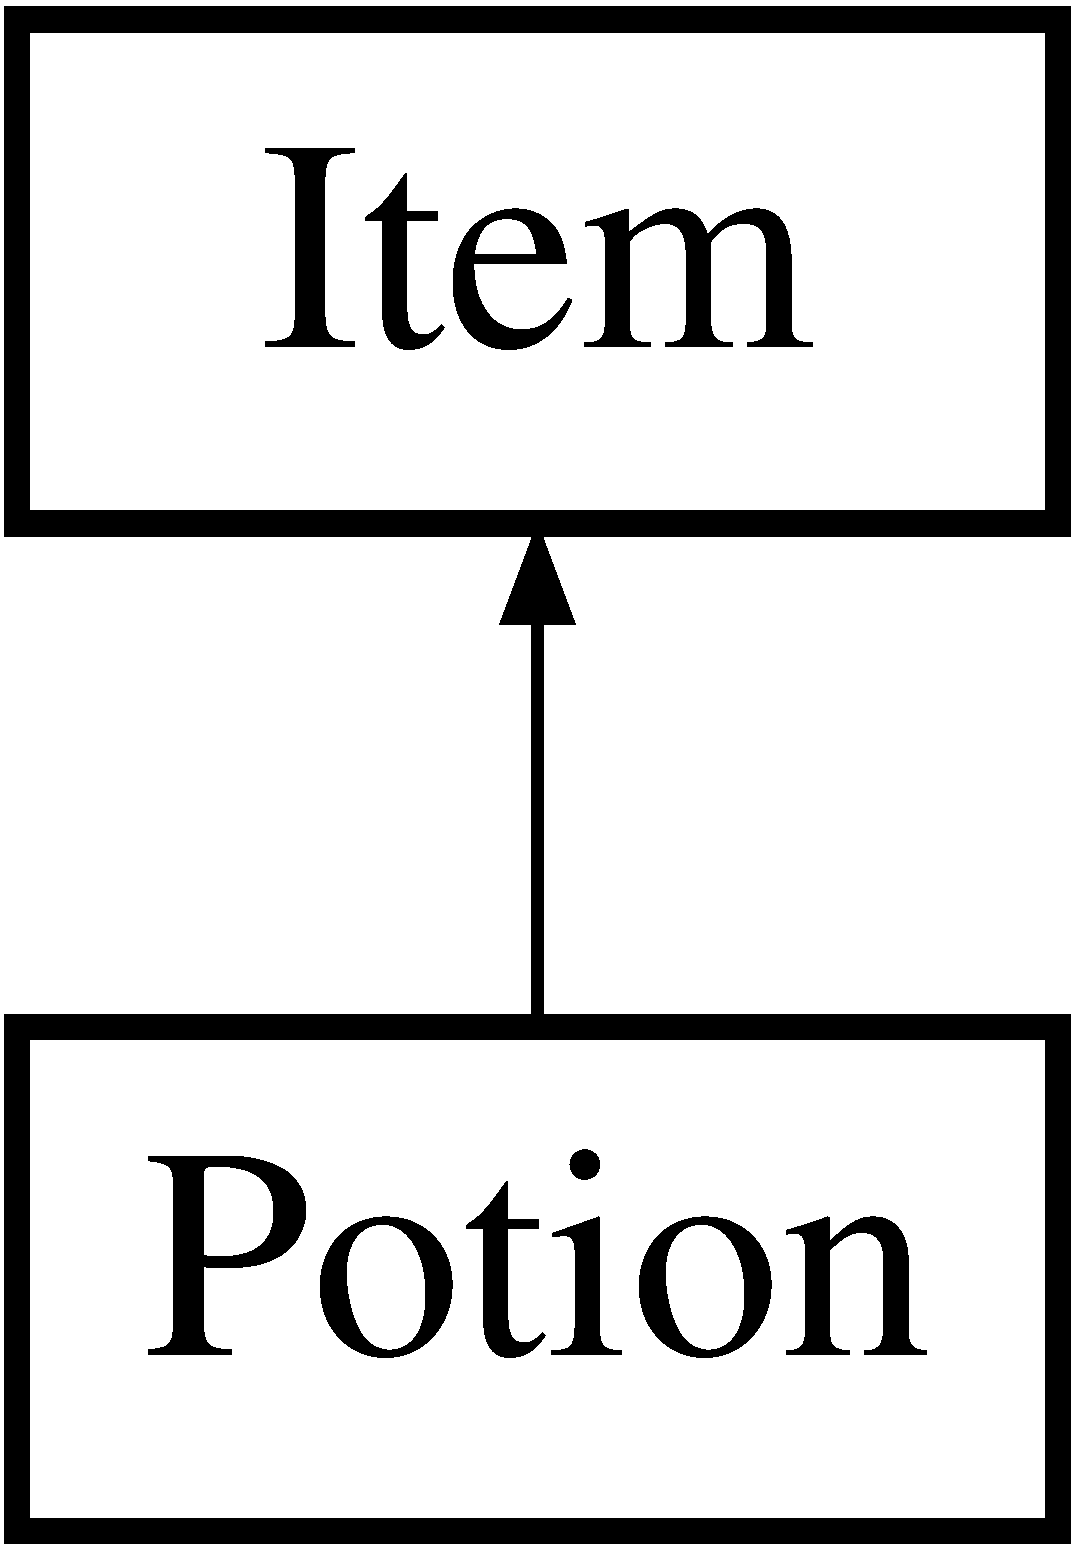
\includegraphics[height=2.000000cm]{class_potion}
\end{center}
\end{figure}
\subsection*{Public Member Functions}
\begin{DoxyCompactItemize}
\item 
\hypertarget{class_potion_ae85fd98bf8c9da25af439bac1581edf4}{}\hyperlink{class_potion_ae85fd98bf8c9da25af439bac1581edf4}{Potion} (string name)\label{class_potion_ae85fd98bf8c9da25af439bac1581edf4}

\begin{DoxyCompactList}\small\item\em Constructs an object \hyperlink{class_potion}{Potion}. \end{DoxyCompactList}\item 
\hypertarget{class_potion_a79ea83f8d6cd83dcfb8bae13760684a8}{}\hyperlink{class_item}{Item} $\ast$ \hyperlink{class_potion_a79ea83f8d6cd83dcfb8bae13760684a8}{clone} (string name)\label{class_potion_a79ea83f8d6cd83dcfb8bae13760684a8}

\begin{DoxyCompactList}\small\item\em Return a new object \hyperlink{class_potion}{Potion}. \end{DoxyCompactList}\end{DoxyCompactItemize}
\subsection*{Additional Inherited Members}


\subsection{Detailed Description}
A \hyperlink{class_potion}{Potion} class inherited from \hyperlink{class_item}{Item} class. 

\hyperlink{class_potion}{Potion} class inherited from \hyperlink{class_item}{Item} class. It contains a constructor and a clone function. It is used to increase the player\textquotesingle{}s health. 

The documentation for this class was generated from the following files\+:\begin{DoxyCompactItemize}
\item 
C\+:/\+Users/\+Mook T/\+Desktop/item/Item\+Prototype.\+h\item 
C\+:/\+Users/\+Mook T/\+Desktop/item/Item\+Prototype.\+cpp\end{DoxyCompactItemize}

\hypertarget{class_json_1_1_reader}{}\section{Json\+:\+:Reader Class Reference}
\label{class_json_1_1_reader}\index{Json\+::\+Reader@{Json\+::\+Reader}}


Unserialize a \href{http://www.json.org}{\tt J\+S\+O\+N} document into a \hyperlink{class_json_1_1_value}{Value}.  




{\ttfamily \#include $<$json.\+h$>$}

\subsection*{Classes}
\begin{DoxyCompactItemize}
\item 
class \hyperlink{class_json_1_1_reader_1_1_error_info}{Error\+Info}
\item 
struct \hyperlink{struct_json_1_1_reader_1_1_structured_error}{Structured\+Error}
\begin{DoxyCompactList}\small\item\em An error tagged with where in the J\+S\+O\+N text it was encountered. \end{DoxyCompactList}\item 
class \hyperlink{class_json_1_1_reader_1_1_token}{Token}
\end{DoxyCompactItemize}
\subsection*{Public Types}
\begin{DoxyCompactItemize}
\item 
\hypertarget{class_json_1_1_reader_a3eec9118f3e9a672ba8348c3a79d0f45}{}typedef char {\bfseries Char}\label{class_json_1_1_reader_a3eec9118f3e9a672ba8348c3a79d0f45}

\item 
\hypertarget{class_json_1_1_reader_a46795b5b272bf79a7730e406cb96375a}{}typedef const Char $\ast$ {\bfseries Location}\label{class_json_1_1_reader_a46795b5b272bf79a7730e406cb96375a}

\end{DoxyCompactItemize}
\subsection*{Public Member Functions}
\begin{DoxyCompactItemize}
\item 
\hypertarget{class_json_1_1_reader_a0b3c4e24c8393354bab57a6ba3ffc27f}{}\hyperlink{class_json_1_1_reader_a0b3c4e24c8393354bab57a6ba3ffc27f}{Reader} ()\label{class_json_1_1_reader_a0b3c4e24c8393354bab57a6ba3ffc27f}

\begin{DoxyCompactList}\small\item\em Constructs a \hyperlink{class_json_1_1_reader}{Reader} allowing all features for parsing. \end{DoxyCompactList}\item 
\hypertarget{class_json_1_1_reader_a45f17831118337309180313e93ac33f8}{}\hyperlink{class_json_1_1_reader_a45f17831118337309180313e93ac33f8}{Reader} (const \hyperlink{class_json_1_1_features}{Features} \&features)\label{class_json_1_1_reader_a45f17831118337309180313e93ac33f8}

\begin{DoxyCompactList}\small\item\em Constructs a \hyperlink{class_json_1_1_reader}{Reader} allowing the specified feature set for parsing. \end{DoxyCompactList}\item 
bool \hyperlink{class_json_1_1_reader_af1da6c976ad1e96c742804c3853eef94}{parse} (const std\+::string \&document, \hyperlink{class_json_1_1_value}{Value} \&root, bool collect\+Comments=true)
\begin{DoxyCompactList}\small\item\em Read a \hyperlink{class_json_1_1_value}{Value} from a \href{http://www.json.org}{\tt J\+S\+O\+N} document. \end{DoxyCompactList}\item 
bool \hyperlink{class_json_1_1_reader_ac71ef2b64c7c27b062052e692af3fb32}{parse} (const char $\ast$begin\+Doc, const char $\ast$end\+Doc, \hyperlink{class_json_1_1_value}{Value} \&root, bool collect\+Comments=true)
\begin{DoxyCompactList}\small\item\em Read a \hyperlink{class_json_1_1_value}{Value} from a \href{http://www.json.org}{\tt J\+S\+O\+N} document. \end{DoxyCompactList}\item 
bool \hyperlink{class_json_1_1_reader_a8d0347e6b47343e4bc68be7ecdb9c4e9}{parse} (std\+::istream \&is, \hyperlink{class_json_1_1_value}{Value} \&root, bool collect\+Comments=true)
\begin{DoxyCompactList}\small\item\em Parse from input stream. \end{DoxyCompactList}\item 
std\+::string \hyperlink{class_json_1_1_reader_afa4a59e962d23c4d1c38b433fc95eefa}{get\+Formated\+Error\+Messages} () const 
\begin{DoxyCompactList}\small\item\em Returns a user friendly string that list errors in the parsed document. \end{DoxyCompactList}\item 
std\+::string \hyperlink{class_json_1_1_reader_a95ab50aa789132e9dee0fc1475c85acf}{get\+Formatted\+Error\+Messages} () const 
\begin{DoxyCompactList}\small\item\em Returns a user friendly string that list errors in the parsed document. \end{DoxyCompactList}\item 
std\+::vector$<$ \hyperlink{struct_json_1_1_reader_1_1_structured_error}{Structured\+Error} $>$ \hyperlink{class_json_1_1_reader_a08c2ea5ffc7d2a9c9e35020835624f0b}{get\+Structured\+Errors} () const 
\begin{DoxyCompactList}\small\item\em Returns a vector of structured erros encounted while parsing. \end{DoxyCompactList}\item 
bool \hyperlink{class_json_1_1_reader_ade6c28e0ef00d8f2e0aa2283f91c3e37}{push\+Error} (const \hyperlink{class_json_1_1_value}{Value} \&value, const std\+::string \&message)
\begin{DoxyCompactList}\small\item\em Add a semantic error message. \end{DoxyCompactList}\item 
bool \hyperlink{class_json_1_1_reader_a9b474233c3a7c688e340e70665d45223}{push\+Error} (const \hyperlink{class_json_1_1_value}{Value} \&value, const std\+::string \&message, const \hyperlink{class_json_1_1_value}{Value} \&extra)
\begin{DoxyCompactList}\small\item\em Add a semantic error message with extra context. \end{DoxyCompactList}\item 
bool \hyperlink{class_json_1_1_reader_a06b52dcc656549506b1ae6f05167ecf4}{good} () const 
\begin{DoxyCompactList}\small\item\em Return whether there are any errors. \end{DoxyCompactList}\end{DoxyCompactItemize}
\subsection*{Private Types}
\begin{DoxyCompactItemize}
\item 
\hypertarget{class_json_1_1_reader_aa35e6ab574dc399a0a645ad98ed66bc9}{}enum {\bfseries Token\+Type} \{ \\*
{\bfseries token\+End\+Of\+Stream} = 0, 
{\bfseries token\+Object\+Begin}, 
{\bfseries token\+Object\+End}, 
{\bfseries token\+Array\+Begin}, 
\\*
{\bfseries token\+Array\+End}, 
{\bfseries token\+String}, 
{\bfseries token\+Number}, 
{\bfseries token\+True}, 
\\*
{\bfseries token\+False}, 
{\bfseries token\+Null}, 
{\bfseries token\+Array\+Separator}, 
{\bfseries token\+Member\+Separator}, 
\\*
{\bfseries token\+Comment}, 
{\bfseries token\+Error}
 \}\label{class_json_1_1_reader_aa35e6ab574dc399a0a645ad98ed66bc9}

\item 
\hypertarget{class_json_1_1_reader_aae51e8f5bab3f067261c842a3ef858e5}{}typedef std\+::deque$<$ \hyperlink{class_json_1_1_reader_1_1_error_info}{Error\+Info} $>$ {\bfseries Errors}\label{class_json_1_1_reader_aae51e8f5bab3f067261c842a3ef858e5}

\item 
\hypertarget{class_json_1_1_reader_a8da2114fe8b8124d41ea2f3434f0171b}{}typedef std\+::stack$<$ \hyperlink{class_json_1_1_value}{Value} $\ast$ $>$ {\bfseries Nodes}\label{class_json_1_1_reader_a8da2114fe8b8124d41ea2f3434f0171b}

\end{DoxyCompactItemize}
\subsection*{Private Member Functions}
\begin{DoxyCompactItemize}
\item 
\hypertarget{class_json_1_1_reader_a7cb0631963cc0fd4ff6ed0f570976864}{}bool {\bfseries read\+Token} (\hyperlink{class_json_1_1_reader_1_1_token}{Token} \&token)\label{class_json_1_1_reader_a7cb0631963cc0fd4ff6ed0f570976864}

\item 
\hypertarget{class_json_1_1_reader_a40d0f69d15aeb2d52ff78d794f5ab8b2}{}void {\bfseries skip\+Spaces} ()\label{class_json_1_1_reader_a40d0f69d15aeb2d52ff78d794f5ab8b2}

\item 
\hypertarget{class_json_1_1_reader_a3e5a7bc6b7b53f2ca8cb9da42f8ffb21}{}bool {\bfseries match} (Location pattern, int pattern\+Length)\label{class_json_1_1_reader_a3e5a7bc6b7b53f2ca8cb9da42f8ffb21}

\item 
\hypertarget{class_json_1_1_reader_ad2690e860a1b3332c5401fb0850ba065}{}bool {\bfseries read\+Comment} ()\label{class_json_1_1_reader_ad2690e860a1b3332c5401fb0850ba065}

\item 
\hypertarget{class_json_1_1_reader_ae0ffe796abdc3c5851589ee500e28c79}{}bool {\bfseries read\+C\+Style\+Comment} ()\label{class_json_1_1_reader_ae0ffe796abdc3c5851589ee500e28c79}

\item 
\hypertarget{class_json_1_1_reader_a6716ef6290b0f469efaf8d379c357967}{}bool {\bfseries read\+Cpp\+Style\+Comment} ()\label{class_json_1_1_reader_a6716ef6290b0f469efaf8d379c357967}

\item 
\hypertarget{class_json_1_1_reader_a6328a0b1994e05118886f9fc9c608643}{}bool {\bfseries read\+String} ()\label{class_json_1_1_reader_a6328a0b1994e05118886f9fc9c608643}

\item 
\hypertarget{class_json_1_1_reader_afb31bfda6bb27d6453057a47655e8363}{}void {\bfseries read\+Number} ()\label{class_json_1_1_reader_afb31bfda6bb27d6453057a47655e8363}

\item 
\hypertarget{class_json_1_1_reader_a47e56844b803d41ec993a83fadf4495c}{}bool {\bfseries read\+Value} ()\label{class_json_1_1_reader_a47e56844b803d41ec993a83fadf4495c}

\item 
\hypertarget{class_json_1_1_reader_a0068eb3d8e86e91f0e4806f60da66b9c}{}bool {\bfseries read\+Object} (\hyperlink{class_json_1_1_reader_1_1_token}{Token} \&token)\label{class_json_1_1_reader_a0068eb3d8e86e91f0e4806f60da66b9c}

\item 
\hypertarget{class_json_1_1_reader_afd9a30c0af205c9f327613f486fae6b8}{}bool {\bfseries read\+Array} (\hyperlink{class_json_1_1_reader_1_1_token}{Token} \&token)\label{class_json_1_1_reader_afd9a30c0af205c9f327613f486fae6b8}

\item 
\hypertarget{class_json_1_1_reader_a442d1f23edf0f4350f5eeab3ee3f7d46}{}bool {\bfseries decode\+Number} (\hyperlink{class_json_1_1_reader_1_1_token}{Token} \&token)\label{class_json_1_1_reader_a442d1f23edf0f4350f5eeab3ee3f7d46}

\item 
\hypertarget{class_json_1_1_reader_a72f426ce3fa384d14aa10e9dd75618f0}{}bool {\bfseries decode\+Number} (\hyperlink{class_json_1_1_reader_1_1_token}{Token} \&token, \hyperlink{class_json_1_1_value}{Value} \&decoded)\label{class_json_1_1_reader_a72f426ce3fa384d14aa10e9dd75618f0}

\item 
\hypertarget{class_json_1_1_reader_aaf736937912f5c9b8d221e57f209e3e0}{}bool {\bfseries decode\+String} (\hyperlink{class_json_1_1_reader_1_1_token}{Token} \&token)\label{class_json_1_1_reader_aaf736937912f5c9b8d221e57f209e3e0}

\item 
\hypertarget{class_json_1_1_reader_a801253570f16e91519652078fb12b8e6}{}bool {\bfseries decode\+String} (\hyperlink{class_json_1_1_reader_1_1_token}{Token} \&token, std\+::string \&decoded)\label{class_json_1_1_reader_a801253570f16e91519652078fb12b8e6}

\item 
\hypertarget{class_json_1_1_reader_a2420bbb7fd6d5d3e7e2fea894dd8f70f}{}bool {\bfseries decode\+Double} (\hyperlink{class_json_1_1_reader_1_1_token}{Token} \&token)\label{class_json_1_1_reader_a2420bbb7fd6d5d3e7e2fea894dd8f70f}

\item 
\hypertarget{class_json_1_1_reader_a5e4a66be7c413bca86078f14df5eb802}{}bool {\bfseries decode\+Double} (\hyperlink{class_json_1_1_reader_1_1_token}{Token} \&token, \hyperlink{class_json_1_1_value}{Value} \&decoded)\label{class_json_1_1_reader_a5e4a66be7c413bca86078f14df5eb802}

\item 
\hypertarget{class_json_1_1_reader_a8fe24db3e9953aef3d637a56447e795c}{}bool {\bfseries decode\+Unicode\+Code\+Point} (\hyperlink{class_json_1_1_reader_1_1_token}{Token} \&token, Location \&current, Location end, unsigned int \&unicode)\label{class_json_1_1_reader_a8fe24db3e9953aef3d637a56447e795c}

\item 
\hypertarget{class_json_1_1_reader_a469cb6f55971d7c41fca2752a3aa5bf7}{}bool {\bfseries decode\+Unicode\+Escape\+Sequence} (\hyperlink{class_json_1_1_reader_1_1_token}{Token} \&token, Location \&current, Location end, unsigned int \&unicode)\label{class_json_1_1_reader_a469cb6f55971d7c41fca2752a3aa5bf7}

\item 
\hypertarget{class_json_1_1_reader_a04a3a13dbc609dfdf9e3c6723e37ff21}{}bool {\bfseries add\+Error} (const std\+::string \&message, \hyperlink{class_json_1_1_reader_1_1_token}{Token} \&token, Location extra=0)\label{class_json_1_1_reader_a04a3a13dbc609dfdf9e3c6723e37ff21}

\item 
\hypertarget{class_json_1_1_reader_a8d4ed03a43082c5ace81ba5b81425eaf}{}bool {\bfseries recover\+From\+Error} (Token\+Type skip\+Until\+Token)\label{class_json_1_1_reader_a8d4ed03a43082c5ace81ba5b81425eaf}

\item 
\hypertarget{class_json_1_1_reader_af47fb7564db6ac21faebaba8cebb41ce}{}bool {\bfseries add\+Error\+And\+Recover} (const std\+::string \&message, \hyperlink{class_json_1_1_reader_1_1_token}{Token} \&token, Token\+Type skip\+Until\+Token)\label{class_json_1_1_reader_af47fb7564db6ac21faebaba8cebb41ce}

\item 
\hypertarget{class_json_1_1_reader_ad922ea5a8ab333084edbb84827861fa3}{}void {\bfseries skip\+Until\+Space} ()\label{class_json_1_1_reader_ad922ea5a8ab333084edbb84827861fa3}

\item 
\hypertarget{class_json_1_1_reader_a85597f763fb0148a17359b6dfc6f7326}{}\hyperlink{class_json_1_1_value}{Value} \& {\bfseries current\+Value} ()\label{class_json_1_1_reader_a85597f763fb0148a17359b6dfc6f7326}

\item 
\hypertarget{class_json_1_1_reader_ab61eb61333cc9ec3afe785663a53ce90}{}Char {\bfseries get\+Next\+Char} ()\label{class_json_1_1_reader_ab61eb61333cc9ec3afe785663a53ce90}

\item 
\hypertarget{class_json_1_1_reader_a20b3023dc422726e2e4ebe41b8ba0515}{}void {\bfseries get\+Location\+Line\+And\+Column} (Location location, int \&line, int \&column) const \label{class_json_1_1_reader_a20b3023dc422726e2e4ebe41b8ba0515}

\item 
\hypertarget{class_json_1_1_reader_ac5b4b5a76d3224871519b0656393b35b}{}std\+::string {\bfseries get\+Location\+Line\+And\+Column} (Location location) const \label{class_json_1_1_reader_ac5b4b5a76d3224871519b0656393b35b}

\item 
\hypertarget{class_json_1_1_reader_aaea3bd62d12ffb6117a61476c0685049}{}void {\bfseries add\+Comment} (Location begin, Location end, \hyperlink{namespace_json_a4fc417c23905b2ae9e2c47d197a45351}{Comment\+Placement} placement)\label{class_json_1_1_reader_aaea3bd62d12ffb6117a61476c0685049}

\item 
\hypertarget{class_json_1_1_reader_a22e677ef400d8223f27e631b4cd4b821}{}void {\bfseries skip\+Comment\+Tokens} (\hyperlink{class_json_1_1_reader_1_1_token}{Token} \&token)\label{class_json_1_1_reader_a22e677ef400d8223f27e631b4cd4b821}

\end{DoxyCompactItemize}
\subsection*{Private Attributes}
\begin{DoxyCompactItemize}
\item 
\hypertarget{class_json_1_1_reader_ada3d2c47699dad662e6d156c8c78a6ac}{}Nodes {\bfseries nodes\+\_\+}\label{class_json_1_1_reader_ada3d2c47699dad662e6d156c8c78a6ac}

\item 
\hypertarget{class_json_1_1_reader_a1bbce45dc4df753bed60c129f4b5147c}{}Errors {\bfseries errors\+\_\+}\label{class_json_1_1_reader_a1bbce45dc4df753bed60c129f4b5147c}

\item 
\hypertarget{class_json_1_1_reader_afde4a4311ae30597da5b6060a8d60542}{}std\+::string {\bfseries document\+\_\+}\label{class_json_1_1_reader_afde4a4311ae30597da5b6060a8d60542}

\item 
\hypertarget{class_json_1_1_reader_a327166839022ea91f0a8290960a8af76}{}Location {\bfseries begin\+\_\+}\label{class_json_1_1_reader_a327166839022ea91f0a8290960a8af76}

\item 
\hypertarget{class_json_1_1_reader_a714793579cbf4ee7c5a7223d2c8d77c1}{}Location {\bfseries end\+\_\+}\label{class_json_1_1_reader_a714793579cbf4ee7c5a7223d2c8d77c1}

\item 
\hypertarget{class_json_1_1_reader_a2f2feb5201a26da7aa133d2f7434479b}{}Location {\bfseries current\+\_\+}\label{class_json_1_1_reader_a2f2feb5201a26da7aa133d2f7434479b}

\item 
\hypertarget{class_json_1_1_reader_a497a114f7b760f1b794b8fff9876615a}{}Location {\bfseries last\+Value\+End\+\_\+}\label{class_json_1_1_reader_a497a114f7b760f1b794b8fff9876615a}

\item 
\hypertarget{class_json_1_1_reader_a87cc75ae5adc6a6755f0ba1c7255ff6c}{}\hyperlink{class_json_1_1_value}{Value} $\ast$ {\bfseries last\+Value\+\_\+}\label{class_json_1_1_reader_a87cc75ae5adc6a6755f0ba1c7255ff6c}

\item 
\hypertarget{class_json_1_1_reader_a240d10ca88620e06a5bd25cc633e9a8a}{}std\+::string {\bfseries comments\+Before\+\_\+}\label{class_json_1_1_reader_a240d10ca88620e06a5bd25cc633e9a8a}

\item 
\hypertarget{class_json_1_1_reader_aa9984ff8f519b5541346157b7aebf97b}{}\hyperlink{class_json_1_1_features}{Features} {\bfseries features\+\_\+}\label{class_json_1_1_reader_aa9984ff8f519b5541346157b7aebf97b}

\item 
\hypertarget{class_json_1_1_reader_a8e9ce743f6004f0596692f0a9ee4626c}{}bool {\bfseries collect\+Comments\+\_\+}\label{class_json_1_1_reader_a8e9ce743f6004f0596692f0a9ee4626c}

\end{DoxyCompactItemize}


\subsection{Detailed Description}
Unserialize a \href{http://www.json.org}{\tt J\+S\+O\+N} document into a \hyperlink{class_json_1_1_value}{Value}. 

\begin{DoxyRefDesc}{Deprecated}
\item[\hyperlink{deprecated__deprecated000005}{Deprecated}]Use \hyperlink{class_json_1_1_char_reader}{Char\+Reader} and \hyperlink{class_json_1_1_char_reader_builder}{Char\+Reader\+Builder}. \end{DoxyRefDesc}


\subsection{Member Function Documentation}
\hypertarget{class_json_1_1_reader_afa4a59e962d23c4d1c38b433fc95eefa}{}\index{Json\+::\+Reader@{Json\+::\+Reader}!get\+Formated\+Error\+Messages@{get\+Formated\+Error\+Messages}}
\index{get\+Formated\+Error\+Messages@{get\+Formated\+Error\+Messages}!Json\+::\+Reader@{Json\+::\+Reader}}
\subsubsection[{get\+Formated\+Error\+Messages() const }]{\setlength{\rightskip}{0pt plus 5cm}std\+::string Json\+::\+Reader\+::get\+Formated\+Error\+Messages (
\begin{DoxyParamCaption}
{}
\end{DoxyParamCaption}
) const}\label{class_json_1_1_reader_afa4a59e962d23c4d1c38b433fc95eefa}


Returns a user friendly string that list errors in the parsed document. 

\begin{DoxyReturn}{Returns}
Formatted error message with the list of errors with their location in the parsed document. An empty string is returned if no error occurred during parsing. 
\end{DoxyReturn}
\begin{DoxyRefDesc}{Deprecated}
\item[\hyperlink{deprecated__deprecated000006}{Deprecated}]Use \hyperlink{class_json_1_1_reader_a95ab50aa789132e9dee0fc1475c85acf}{get\+Formatted\+Error\+Messages()} instead (typo fix). \end{DoxyRefDesc}
\hypertarget{class_json_1_1_reader_a95ab50aa789132e9dee0fc1475c85acf}{}\index{Json\+::\+Reader@{Json\+::\+Reader}!get\+Formatted\+Error\+Messages@{get\+Formatted\+Error\+Messages}}
\index{get\+Formatted\+Error\+Messages@{get\+Formatted\+Error\+Messages}!Json\+::\+Reader@{Json\+::\+Reader}}
\subsubsection[{get\+Formatted\+Error\+Messages() const }]{\setlength{\rightskip}{0pt plus 5cm}std\+::string Json\+::\+Reader\+::get\+Formatted\+Error\+Messages (
\begin{DoxyParamCaption}
{}
\end{DoxyParamCaption}
) const}\label{class_json_1_1_reader_a95ab50aa789132e9dee0fc1475c85acf}


Returns a user friendly string that list errors in the parsed document. 

\begin{DoxyReturn}{Returns}
Formatted error message with the list of errors with their location in the parsed document. An empty string is returned if no error occurred during parsing. 
\end{DoxyReturn}
\hypertarget{class_json_1_1_reader_a08c2ea5ffc7d2a9c9e35020835624f0b}{}\index{Json\+::\+Reader@{Json\+::\+Reader}!get\+Structured\+Errors@{get\+Structured\+Errors}}
\index{get\+Structured\+Errors@{get\+Structured\+Errors}!Json\+::\+Reader@{Json\+::\+Reader}}
\subsubsection[{get\+Structured\+Errors() const }]{\setlength{\rightskip}{0pt plus 5cm}std\+::vector$<$ {\bf Reader\+::\+Structured\+Error} $>$ Json\+::\+Reader\+::get\+Structured\+Errors (
\begin{DoxyParamCaption}
{}
\end{DoxyParamCaption}
) const}\label{class_json_1_1_reader_a08c2ea5ffc7d2a9c9e35020835624f0b}


Returns a vector of structured erros encounted while parsing. 

\begin{DoxyReturn}{Returns}
A (possibly empty) vector of \hyperlink{struct_json_1_1_reader_1_1_structured_error}{Structured\+Error} objects. Currently only one error can be returned, but the caller should tolerate multiple errors. This can occur if the parser recovers from a non-\/fatal parse error and then encounters additional errors. 
\end{DoxyReturn}
\hypertarget{class_json_1_1_reader_a06b52dcc656549506b1ae6f05167ecf4}{}\index{Json\+::\+Reader@{Json\+::\+Reader}!good@{good}}
\index{good@{good}!Json\+::\+Reader@{Json\+::\+Reader}}
\subsubsection[{good() const }]{\setlength{\rightskip}{0pt plus 5cm}bool Json\+::\+Reader\+::good (
\begin{DoxyParamCaption}
{}
\end{DoxyParamCaption}
) const}\label{class_json_1_1_reader_a06b52dcc656549506b1ae6f05167ecf4}


Return whether there are any errors. 

\begin{DoxyReturn}{Returns}
{\ttfamily true} if there are no errors to report {\ttfamily false} if errors have occurred. 
\end{DoxyReturn}
\hypertarget{class_json_1_1_reader_af1da6c976ad1e96c742804c3853eef94}{}\index{Json\+::\+Reader@{Json\+::\+Reader}!parse@{parse}}
\index{parse@{parse}!Json\+::\+Reader@{Json\+::\+Reader}}
\subsubsection[{parse(const std\+::string \&document, Value \&root, bool collect\+Comments=true)}]{\setlength{\rightskip}{0pt plus 5cm}bool Json\+::\+Reader\+::parse (
\begin{DoxyParamCaption}
\item[{const std\+::string \&}]{document, }
\item[{{\bf Value} \&}]{root, }
\item[{bool}]{collect\+Comments = {\ttfamily true}}
\end{DoxyParamCaption}
)}\label{class_json_1_1_reader_af1da6c976ad1e96c742804c3853eef94}


Read a \hyperlink{class_json_1_1_value}{Value} from a \href{http://www.json.org}{\tt J\+S\+O\+N} document. 


\begin{DoxyParams}{Parameters}
{\em document} & U\+T\+F-\/8 encoded string containing the document to read. \\
\hline
{\em root} & \mbox{[}out\mbox{]} Contains the root value of the document if it was successfully parsed. \\
\hline
{\em collect\+Comments} & {\ttfamily true} to collect comment and allow writing them back during serialization, {\ttfamily false} to discard comments. This parameter is ignored if \hyperlink{class_json_1_1_features_a33afd389719624b6bdb23950b3c346c9}{Features\+::allow\+Comments\+\_\+} is {\ttfamily false}. \\
\hline
\end{DoxyParams}
\begin{DoxyReturn}{Returns}
{\ttfamily true} if the document was successfully parsed, {\ttfamily false} if an error occurred. 
\end{DoxyReturn}
\hypertarget{class_json_1_1_reader_ac71ef2b64c7c27b062052e692af3fb32}{}\index{Json\+::\+Reader@{Json\+::\+Reader}!parse@{parse}}
\index{parse@{parse}!Json\+::\+Reader@{Json\+::\+Reader}}
\subsubsection[{parse(const char $\ast$begin\+Doc, const char $\ast$end\+Doc, Value \&root, bool collect\+Comments=true)}]{\setlength{\rightskip}{0pt plus 5cm}bool Json\+::\+Reader\+::parse (
\begin{DoxyParamCaption}
\item[{const char $\ast$}]{begin\+Doc, }
\item[{const char $\ast$}]{end\+Doc, }
\item[{{\bf Value} \&}]{root, }
\item[{bool}]{collect\+Comments = {\ttfamily true}}
\end{DoxyParamCaption}
)}\label{class_json_1_1_reader_ac71ef2b64c7c27b062052e692af3fb32}


Read a \hyperlink{class_json_1_1_value}{Value} from a \href{http://www.json.org}{\tt J\+S\+O\+N} document. 


\begin{DoxyParams}{Parameters}
{\em begin\+Doc} & Pointer on the beginning of the U\+T\+F-\/8 encoded string of the document to read. \\
\hline
{\em end\+Doc} & Pointer on the end of the U\+T\+F-\/8 encoded string of the document to read. Must be $>$= begin\+Doc. \\
\hline
{\em root} & \mbox{[}out\mbox{]} Contains the root value of the document if it was successfully parsed. \\
\hline
{\em collect\+Comments} & {\ttfamily true} to collect comment and allow writing them back during serialization, {\ttfamily false} to discard comments. This parameter is ignored if \hyperlink{class_json_1_1_features_a33afd389719624b6bdb23950b3c346c9}{Features\+::allow\+Comments\+\_\+} is {\ttfamily false}. \\
\hline
\end{DoxyParams}
\begin{DoxyReturn}{Returns}
{\ttfamily true} if the document was successfully parsed, {\ttfamily false} if an error occurred. 
\end{DoxyReturn}
\hypertarget{class_json_1_1_reader_a8d0347e6b47343e4bc68be7ecdb9c4e9}{}\index{Json\+::\+Reader@{Json\+::\+Reader}!parse@{parse}}
\index{parse@{parse}!Json\+::\+Reader@{Json\+::\+Reader}}
\subsubsection[{parse(std\+::istream \&is, Value \&root, bool collect\+Comments=true)}]{\setlength{\rightskip}{0pt plus 5cm}bool Json\+::\+Reader\+::parse (
\begin{DoxyParamCaption}
\item[{std\+::istream \&}]{is, }
\item[{{\bf Value} \&}]{root, }
\item[{bool}]{collect\+Comments = {\ttfamily true}}
\end{DoxyParamCaption}
)}\label{class_json_1_1_reader_a8d0347e6b47343e4bc68be7ecdb9c4e9}


Parse from input stream. 

\begin{DoxySeeAlso}{See also}
\hyperlink{namespace_json_a4d245ef719cc0853e8e78eb5f99c16e5}{Json\+::operator$>$$>$(std\+::istream\&, Json\+::\+Value\&)}. 
\end{DoxySeeAlso}
\hypertarget{class_json_1_1_reader_ade6c28e0ef00d8f2e0aa2283f91c3e37}{}\index{Json\+::\+Reader@{Json\+::\+Reader}!push\+Error@{push\+Error}}
\index{push\+Error@{push\+Error}!Json\+::\+Reader@{Json\+::\+Reader}}
\subsubsection[{push\+Error(const Value \&value, const std\+::string \&message)}]{\setlength{\rightskip}{0pt plus 5cm}bool Json\+::\+Reader\+::push\+Error (
\begin{DoxyParamCaption}
\item[{const {\bf Value} \&}]{value, }
\item[{const std\+::string \&}]{message}
\end{DoxyParamCaption}
)}\label{class_json_1_1_reader_ade6c28e0ef00d8f2e0aa2283f91c3e37}


Add a semantic error message. 


\begin{DoxyParams}{Parameters}
{\em value} & J\+S\+O\+N \hyperlink{class_json_1_1_value}{Value} location associated with the error \\
\hline
{\em message} & The error message. \\
\hline
\end{DoxyParams}
\begin{DoxyReturn}{Returns}
{\ttfamily true} if the error was successfully added, {\ttfamily false} if the \hyperlink{class_json_1_1_value}{Value} offset exceeds the document size. 
\end{DoxyReturn}
\hypertarget{class_json_1_1_reader_a9b474233c3a7c688e340e70665d45223}{}\index{Json\+::\+Reader@{Json\+::\+Reader}!push\+Error@{push\+Error}}
\index{push\+Error@{push\+Error}!Json\+::\+Reader@{Json\+::\+Reader}}
\subsubsection[{push\+Error(const Value \&value, const std\+::string \&message, const Value \&extra)}]{\setlength{\rightskip}{0pt plus 5cm}bool Json\+::\+Reader\+::push\+Error (
\begin{DoxyParamCaption}
\item[{const {\bf Value} \&}]{value, }
\item[{const std\+::string \&}]{message, }
\item[{const {\bf Value} \&}]{extra}
\end{DoxyParamCaption}
)}\label{class_json_1_1_reader_a9b474233c3a7c688e340e70665d45223}


Add a semantic error message with extra context. 


\begin{DoxyParams}{Parameters}
{\em value} & J\+S\+O\+N \hyperlink{class_json_1_1_value}{Value} location associated with the error \\
\hline
{\em message} & The error message. \\
\hline
{\em extra} & Additional J\+S\+O\+N \hyperlink{class_json_1_1_value}{Value} location to contextualize the error \\
\hline
\end{DoxyParams}
\begin{DoxyReturn}{Returns}
{\ttfamily true} if the error was successfully added, {\ttfamily false} if either \hyperlink{class_json_1_1_value}{Value} offset exceeds the document size. 
\end{DoxyReturn}


The documentation for this class was generated from the following files\+:\begin{DoxyCompactItemize}
\item 
C\+:/\+Users/\+Mook T/\+Desktop/item/json.\+h\item 
C\+:/\+Users/\+Mook T/\+Desktop/item/jsoncpp.\+cpp\end{DoxyCompactItemize}

\hypertarget{class_json_1_1_runtime_error}{}\section{Json\+:\+:Runtime\+Error Class Reference}
\label{class_json_1_1_runtime_error}\index{Json\+::\+Runtime\+Error@{Json\+::\+Runtime\+Error}}


{\ttfamily \#include $<$json.\+h$>$}

Inheritance diagram for Json\+:\+:Runtime\+Error\+:\begin{figure}[H]
\begin{center}
\leavevmode
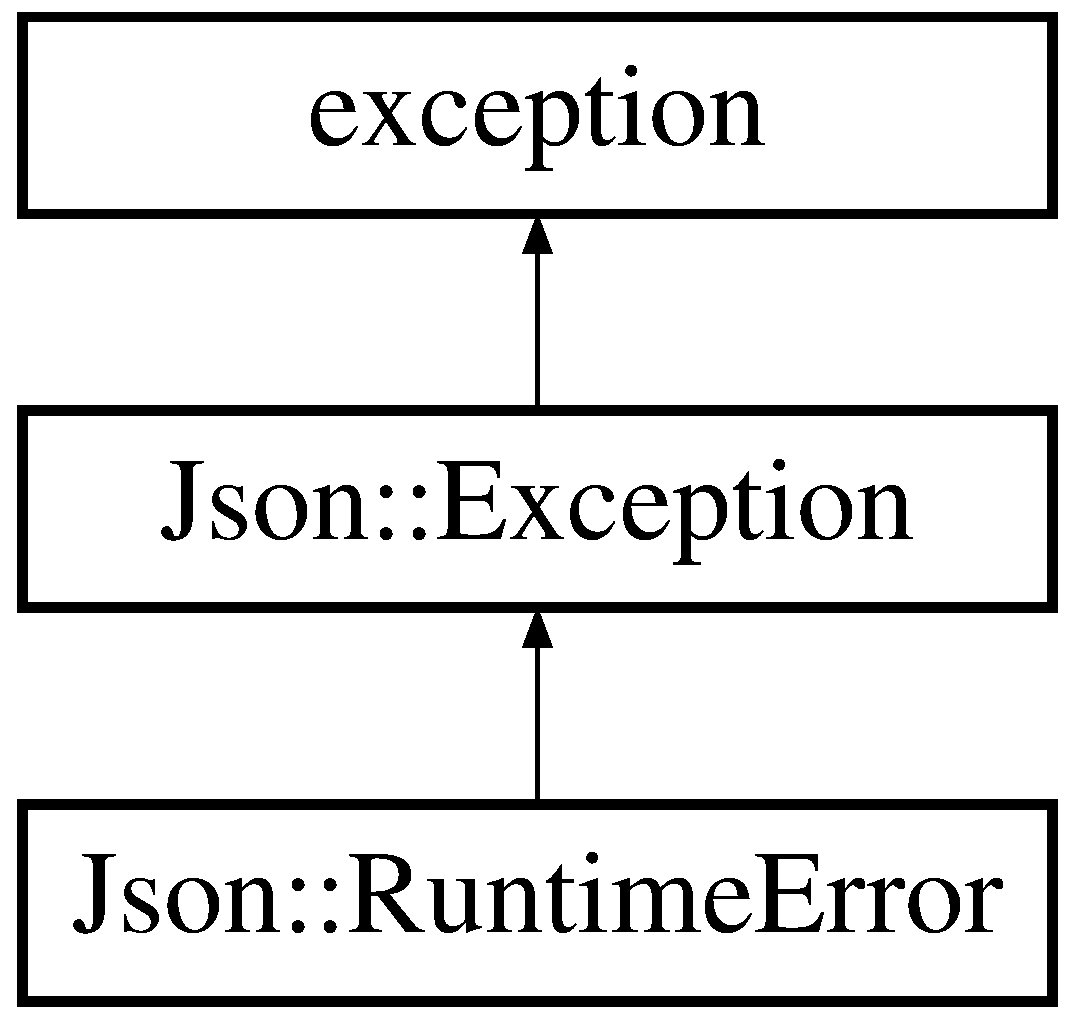
\includegraphics[height=3.000000cm]{class_json_1_1_runtime_error}
\end{center}
\end{figure}
\subsection*{Public Member Functions}
\begin{DoxyCompactItemize}
\item 
\hypertarget{class_json_1_1_runtime_error_ae4f102d5c1efb773887efc8c7911e6f8}{}{\bfseries Runtime\+Error} (std\+::string const \&msg)\label{class_json_1_1_runtime_error_ae4f102d5c1efb773887efc8c7911e6f8}

\end{DoxyCompactItemize}
\subsection*{Additional Inherited Members}


\subsection{Detailed Description}
Exceptions which the user cannot easily avoid.

E.\+g. out-\/of-\/memory (when we use malloc), stack-\/overflow, malicious input

\begin{DoxyRemark}{Remarks}
derived from \hyperlink{class_json_1_1_exception}{Json\+::\+Exception} 
\end{DoxyRemark}


The documentation for this class was generated from the following files\+:\begin{DoxyCompactItemize}
\item 
C\+:/\+Users/\+Mook T/\+Desktop/item/json.\+h\item 
C\+:/\+Users/\+Mook T/\+Desktop/item/jsoncpp.\+cpp\end{DoxyCompactItemize}

\hypertarget{class_json_1_1_static_string}{}\section{Json\+:\+:Static\+String Class Reference}
\label{class_json_1_1_static_string}\index{Json\+::\+Static\+String@{Json\+::\+Static\+String}}


Lightweight wrapper to tag static string.  




{\ttfamily \#include $<$json.\+h$>$}

\subsection*{Public Member Functions}
\begin{DoxyCompactItemize}
\item 
\hypertarget{class_json_1_1_static_string_afb6baf1ec078ce76f0b0f9b39d19437f}{}{\bfseries Static\+String} (const char $\ast$czstring)\label{class_json_1_1_static_string_afb6baf1ec078ce76f0b0f9b39d19437f}

\item 
\hypertarget{class_json_1_1_static_string_ac2b334d46bbea4c0227e508fc66433e9}{}{\bfseries operator const char $\ast$} () const \label{class_json_1_1_static_string_ac2b334d46bbea4c0227e508fc66433e9}

\item 
\hypertarget{class_json_1_1_static_string_ab86fc6a3183adf12fdba4b370acf1754}{}const char $\ast$ {\bfseries c\+\_\+str} () const \label{class_json_1_1_static_string_ab86fc6a3183adf12fdba4b370acf1754}

\end{DoxyCompactItemize}
\subsection*{Private Attributes}
\begin{DoxyCompactItemize}
\item 
\hypertarget{class_json_1_1_static_string_a9f0d9e8caee8f8db14e2c8c24760dffd}{}const char $\ast$ {\bfseries c\+\_\+str\+\_\+}\label{class_json_1_1_static_string_a9f0d9e8caee8f8db14e2c8c24760dffd}

\end{DoxyCompactItemize}


\subsection{Detailed Description}
Lightweight wrapper to tag static string. 

\hyperlink{class_json_1_1_value}{Value} constructor and object\+Value member assignement takes advantage of the \hyperlink{class_json_1_1_static_string}{Static\+String} and avoid the cost of string duplication when storing the string or the member name.

Example of usage\+: 
\begin{DoxyCode}
\hyperlink{class_json_1_1_value}{Json::Value} aValue( StaticString(\textcolor{stringliteral}{"some text"}) );
\hyperlink{class_json_1_1_value}{Json::Value} object;
\textcolor{keyword}{static} \textcolor{keyword}{const} StaticString code(\textcolor{stringliteral}{"code"});
\textcolor{keywordtype}{object}[code] = 1234;
\end{DoxyCode}
 

The documentation for this class was generated from the following file\+:\begin{DoxyCompactItemize}
\item 
C\+:/\+Users/\+Mook T/\+Desktop/item/json.\+h\end{DoxyCompactItemize}

\hypertarget{class_json_1_1_stream_writer}{}\section{Json\+:\+:Stream\+Writer Class Reference}
\label{class_json_1_1_stream_writer}\index{Json\+::\+Stream\+Writer@{Json\+::\+Stream\+Writer}}


{\ttfamily \#include $<$json.\+h$>$}

Inheritance diagram for Json\+:\+:Stream\+Writer\+:\begin{figure}[H]
\begin{center}
\leavevmode
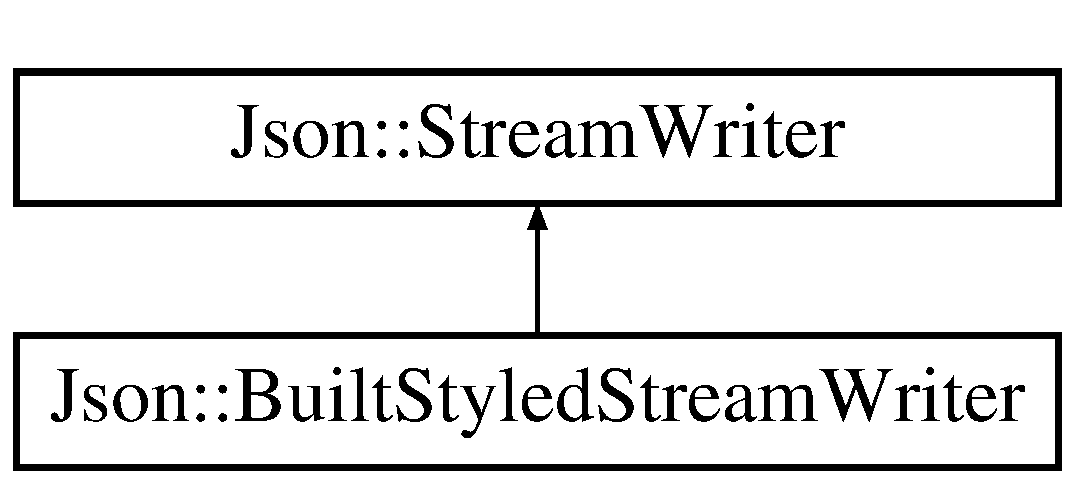
\includegraphics[height=2.000000cm]{class_json_1_1_stream_writer}
\end{center}
\end{figure}
\subsection*{Classes}
\begin{DoxyCompactItemize}
\item 
class \hyperlink{class_json_1_1_stream_writer_1_1_factory}{Factory}
\begin{DoxyCompactList}\small\item\em A simple abstract factory. \end{DoxyCompactList}\end{DoxyCompactItemize}
\subsection*{Public Member Functions}
\begin{DoxyCompactItemize}
\item 
virtual int \hyperlink{class_json_1_1_stream_writer_a237368cf13b41decc015640d25f176ab}{write} (\hyperlink{class_json_1_1_value}{Value} const \&root, std\+::ostream $\ast$sout)=0
\end{DoxyCompactItemize}
\subsection*{Protected Attributes}
\begin{DoxyCompactItemize}
\item 
\hypertarget{class_json_1_1_stream_writer_ac087569ccd2b5a22348cae92ec2a8996}{}std\+::ostream $\ast$ {\bfseries sout\+\_\+}\label{class_json_1_1_stream_writer_ac087569ccd2b5a22348cae92ec2a8996}

\end{DoxyCompactItemize}


\subsection{Detailed Description}
Usage\+: 
\begin{DoxyCode}
\textcolor{keyword}{using namespace }\hyperlink{namespace_json}{Json};
\textcolor{keywordtype}{void} writeToStdout(\hyperlink{class_json_1_1_stream_writer_1_1_factory}{StreamWriter::Factory} \textcolor{keyword}{const}& factory, 
      \hyperlink{class_json_1_1_value}{Value} \textcolor{keyword}{const}& value) \{
  std::unique\_ptr<StreamWriter> \textcolor{keyword}{const} writer(
    factory.\hyperlink{class_json_1_1_stream_writer_1_1_factory_a0fca8d713eb8949ca3ebb35e67f23b1a}{newStreamWriter}());
  writer->write(value, &std::cout);
  std::cout << std::endl;  \textcolor{comment}{// add lf and flush}
\}
\end{DoxyCode}
 

\subsection{Member Function Documentation}
\hypertarget{class_json_1_1_stream_writer_a237368cf13b41decc015640d25f176ab}{}\index{Json\+::\+Stream\+Writer@{Json\+::\+Stream\+Writer}!write@{write}}
\index{write@{write}!Json\+::\+Stream\+Writer@{Json\+::\+Stream\+Writer}}
\subsubsection[{write(\+Value const \&root, std\+::ostream $\ast$sout)=0}]{\setlength{\rightskip}{0pt plus 5cm}virtual int Json\+::\+Stream\+Writer\+::write (
\begin{DoxyParamCaption}
\item[{{\bf Value} const \&}]{root, }
\item[{std\+::ostream $\ast$}]{sout}
\end{DoxyParamCaption}
)\hspace{0.3cm}{\ttfamily [pure virtual]}}\label{class_json_1_1_stream_writer_a237368cf13b41decc015640d25f176ab}
Write \hyperlink{class_json_1_1_value}{Value} into document as configured in sub-\/class. Do not take ownership of sout, but maintain a reference during function. \begin{DoxyPrecond}{Precondition}
sout != N\+U\+L\+L 
\end{DoxyPrecond}
\begin{DoxyReturn}{Returns}
zero on success (For now, we always return zero, so check the stream instead.) 
\end{DoxyReturn}

\begin{DoxyExceptions}{Exceptions}
{\em std\+::exception} & possibly, depending on configuration \\
\hline
\end{DoxyExceptions}


Implemented in \hyperlink{struct_json_1_1_built_styled_stream_writer_ab8810d938c35c8442cbffcd001628cd0}{Json\+::\+Built\+Styled\+Stream\+Writer}.



The documentation for this class was generated from the following files\+:\begin{DoxyCompactItemize}
\item 
C\+:/\+Users/\+Mook T/\+Desktop/item/json.\+h\item 
C\+:/\+Users/\+Mook T/\+Desktop/item/jsoncpp.\+cpp\end{DoxyCompactItemize}

\hypertarget{class_json_1_1_stream_writer_builder}{}\section{Json\+:\+:Stream\+Writer\+Builder Class Reference}
\label{class_json_1_1_stream_writer_builder}\index{Json\+::\+Stream\+Writer\+Builder@{Json\+::\+Stream\+Writer\+Builder}}


Build a \hyperlink{class_json_1_1_stream_writer}{Stream\+Writer} implementation.  




{\ttfamily \#include $<$json.\+h$>$}

Inheritance diagram for Json\+:\+:Stream\+Writer\+Builder\+:\begin{figure}[H]
\begin{center}
\leavevmode
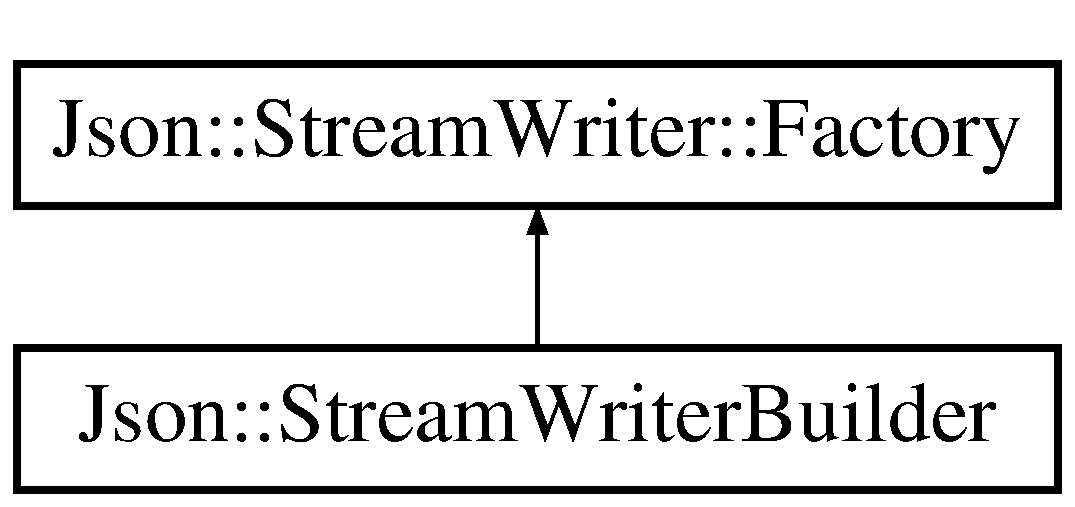
\includegraphics[height=2.000000cm]{class_json_1_1_stream_writer_builder}
\end{center}
\end{figure}
\subsection*{Public Member Functions}
\begin{DoxyCompactItemize}
\item 
\hyperlink{class_json_1_1_stream_writer}{Stream\+Writer} $\ast$ \hyperlink{class_json_1_1_stream_writer_builder_a96c85792f6680835094917ee93915e4b}{new\+Stream\+Writer} () const 
\item 
bool \hyperlink{class_json_1_1_stream_writer_builder_aa1dfed085a3d369e953e4a3c34da009e}{validate} (\hyperlink{class_json_1_1_value}{Json\+::\+Value} $\ast$invalid) const 
\item 
\hyperlink{class_json_1_1_value}{Value} \& \hyperlink{class_json_1_1_stream_writer_builder_aa010a8a04a92343179f64a5dbb5df340}{operator\mbox{[}$\,$\mbox{]}} (std\+::string key)
\end{DoxyCompactItemize}
\subsection*{Static Public Member Functions}
\begin{DoxyCompactItemize}
\item 
static void \hyperlink{class_json_1_1_stream_writer_builder_a53bf106b141e28637b01ad0ecd2acbf6}{set\+Defaults} (\hyperlink{class_json_1_1_value}{Json\+::\+Value} $\ast$settings)
\end{DoxyCompactItemize}
\subsection*{Public Attributes}
\begin{DoxyCompactItemize}
\item 
\hyperlink{class_json_1_1_value}{Json\+::\+Value} \hyperlink{class_json_1_1_stream_writer_builder_a79bdf2e639a52f4e758c0b95bd1d3423}{settings\+\_\+}
\end{DoxyCompactItemize}


\subsection{Detailed Description}
Build a \hyperlink{class_json_1_1_stream_writer}{Stream\+Writer} implementation. 

Usage\+: 
\begin{DoxyCode}
\textcolor{keyword}{using namespace }\hyperlink{namespace_json}{Json};
\hyperlink{class_json_1_1_value}{Value} value = ...;
\hyperlink{class_json_1_1_stream_writer_builder}{StreamWriterBuilder} builder;
builder[\textcolor{stringliteral}{"commentStyle"}] = \textcolor{stringliteral}{"None"};
builder[\textcolor{stringliteral}{"indentation"}] = \textcolor{stringliteral}{"   "};  \textcolor{comment}{// or whatever you like}
std::unique\_ptr<Json::StreamWriter> writer(
    builder.\hyperlink{class_json_1_1_stream_writer_builder_a96c85792f6680835094917ee93915e4b}{newStreamWriter}());
writer->write(value, &std::cout);
std::cout << std::endl;  \textcolor{comment}{// add lf and flush}
\end{DoxyCode}
 

\subsection{Member Function Documentation}
\hypertarget{class_json_1_1_stream_writer_builder_a96c85792f6680835094917ee93915e4b}{}\index{Json\+::\+Stream\+Writer\+Builder@{Json\+::\+Stream\+Writer\+Builder}!new\+Stream\+Writer@{new\+Stream\+Writer}}
\index{new\+Stream\+Writer@{new\+Stream\+Writer}!Json\+::\+Stream\+Writer\+Builder@{Json\+::\+Stream\+Writer\+Builder}}
\subsubsection[{new\+Stream\+Writer() const }]{\setlength{\rightskip}{0pt plus 5cm}{\bf Stream\+Writer} $\ast$ Json\+::\+Stream\+Writer\+Builder\+::new\+Stream\+Writer (
\begin{DoxyParamCaption}
{}
\end{DoxyParamCaption}
) const\hspace{0.3cm}{\ttfamily [virtual]}}\label{class_json_1_1_stream_writer_builder_a96c85792f6680835094917ee93915e4b}

\begin{DoxyExceptions}{Exceptions}
{\em std\+::exception} & if something goes wrong (e.\+g. invalid settings) \\
\hline
\end{DoxyExceptions}


Implements \hyperlink{class_json_1_1_stream_writer_1_1_factory_a0fca8d713eb8949ca3ebb35e67f23b1a}{Json\+::\+Stream\+Writer\+::\+Factory}.

\hypertarget{class_json_1_1_stream_writer_builder_aa010a8a04a92343179f64a5dbb5df340}{}\index{Json\+::\+Stream\+Writer\+Builder@{Json\+::\+Stream\+Writer\+Builder}!operator\mbox{[}$\,$\mbox{]}@{operator[]}}
\index{operator\mbox{[}$\,$\mbox{]}@{operator[]}!Json\+::\+Stream\+Writer\+Builder@{Json\+::\+Stream\+Writer\+Builder}}
\subsubsection[{operator[](std\+::string key)}]{\setlength{\rightskip}{0pt plus 5cm}{\bf Value} \& Json\+::\+Stream\+Writer\+Builder\+::operator\mbox{[}$\,$\mbox{]} (
\begin{DoxyParamCaption}
\item[{std\+::string}]{key}
\end{DoxyParamCaption}
)}\label{class_json_1_1_stream_writer_builder_aa010a8a04a92343179f64a5dbb5df340}
A simple way to update a specific setting. \hypertarget{class_json_1_1_stream_writer_builder_a53bf106b141e28637b01ad0ecd2acbf6}{}\index{Json\+::\+Stream\+Writer\+Builder@{Json\+::\+Stream\+Writer\+Builder}!set\+Defaults@{set\+Defaults}}
\index{set\+Defaults@{set\+Defaults}!Json\+::\+Stream\+Writer\+Builder@{Json\+::\+Stream\+Writer\+Builder}}
\subsubsection[{set\+Defaults(\+Json\+::\+Value $\ast$settings)}]{\setlength{\rightskip}{0pt plus 5cm}void Json\+::\+Stream\+Writer\+Builder\+::set\+Defaults (
\begin{DoxyParamCaption}
\item[{{\bf Json\+::\+Value} $\ast$}]{settings}
\end{DoxyParamCaption}
)\hspace{0.3cm}{\ttfamily [static]}}\label{class_json_1_1_stream_writer_builder_a53bf106b141e28637b01ad0ecd2acbf6}
Called by ctor, but you can use this to reset settings\+\_\+. \begin{DoxyPrecond}{Precondition}
\textquotesingle{}settings\textquotesingle{} != N\+U\+L\+L (but Json\+::null is fine) 
\end{DoxyPrecond}
\begin{DoxyRemark}{Remarks}
Defaults\+: 
\begin{DoxyCodeInclude}
\end{DoxyCodeInclude}

\end{DoxyRemark}
\mbox{[}Stream\+Writer\+Builder\+Defaults\mbox{]}

\mbox{[}Stream\+Writer\+Builder\+Defaults\mbox{]} \hypertarget{class_json_1_1_stream_writer_builder_aa1dfed085a3d369e953e4a3c34da009e}{}\index{Json\+::\+Stream\+Writer\+Builder@{Json\+::\+Stream\+Writer\+Builder}!validate@{validate}}
\index{validate@{validate}!Json\+::\+Stream\+Writer\+Builder@{Json\+::\+Stream\+Writer\+Builder}}
\subsubsection[{validate(\+Json\+::\+Value $\ast$invalid) const }]{\setlength{\rightskip}{0pt plus 5cm}bool Json\+::\+Stream\+Writer\+Builder\+::validate (
\begin{DoxyParamCaption}
\item[{{\bf Json\+::\+Value} $\ast$}]{invalid}
\end{DoxyParamCaption}
) const}\label{class_json_1_1_stream_writer_builder_aa1dfed085a3d369e953e4a3c34da009e}
\begin{DoxyReturn}{Returns}
true if \textquotesingle{}settings\textquotesingle{} are legal and consistent; otherwise, indicate bad settings via \textquotesingle{}invalid\textquotesingle{}. 
\end{DoxyReturn}


\subsection{Member Data Documentation}
\hypertarget{class_json_1_1_stream_writer_builder_a79bdf2e639a52f4e758c0b95bd1d3423}{}\index{Json\+::\+Stream\+Writer\+Builder@{Json\+::\+Stream\+Writer\+Builder}!settings\+\_\+@{settings\+\_\+}}
\index{settings\+\_\+@{settings\+\_\+}!Json\+::\+Stream\+Writer\+Builder@{Json\+::\+Stream\+Writer\+Builder}}
\subsubsection[{settings\+\_\+}]{\setlength{\rightskip}{0pt plus 5cm}{\bf Json\+::\+Value} Json\+::\+Stream\+Writer\+Builder\+::settings\+\_\+}\label{class_json_1_1_stream_writer_builder_a79bdf2e639a52f4e758c0b95bd1d3423}
Configuration of this builder. Available settings (case-\/sensitive)\+:
\begin{DoxyItemize}
\item \char`\"{}comment\+Style\char`\"{}\+: \char`\"{}\+None\char`\"{} or \char`\"{}\+All\char`\"{}
\item \char`\"{}indentation\char`\"{}\+: \char`\"{}$<$anything$>$\char`\"{}
\item \char`\"{}enable\+Y\+A\+M\+L\+Compatibility\char`\"{}\+: false or true
\begin{DoxyItemize}
\item slightly change the whitespace around colons
\end{DoxyItemize}
\item \char`\"{}drop\+Null\+Placeholders\char`\"{}\+: false or true
\begin{DoxyItemize}
\item Drop the \char`\"{}null\char`\"{} string from the writer\textquotesingle{}s output for null\+Values. Strictly speaking, this is not valid J\+S\+O\+N. But when the output is being fed to a browser\textquotesingle{}s Javascript, it makes for smaller output and the browser can handle the output just fine.
\end{DoxyItemize}
\item \char`\"{}use\+Special\+Floats\char`\"{}\+: false or true
\begin{DoxyItemize}
\item If true, outputs non-\/finite floating point values in the following way\+: Na\+N values as \char`\"{}\+Na\+N\char`\"{}, positive infinity as \char`\"{}\+Infinity\char`\"{}, and negative infinity as \char`\"{}-\/\+Infinity\char`\"{}.
\end{DoxyItemize}
\end{DoxyItemize}

You can examine \textquotesingle{}settings\+\_\+` yourself to see the defaults. You can also write and read them just like any J\+S\+O\+N \hyperlink{class_json_1_1_value}{Value}. \begin{DoxySeeAlso}{See also}
\hyperlink{class_json_1_1_stream_writer_builder_a53bf106b141e28637b01ad0ecd2acbf6}{set\+Defaults()} 
\end{DoxySeeAlso}


The documentation for this class was generated from the following files\+:\begin{DoxyCompactItemize}
\item 
C\+:/\+Users/\+Mook T/\+Desktop/item/json.\+h\item 
C\+:/\+Users/\+Mook T/\+Desktop/item/jsoncpp.\+cpp\end{DoxyCompactItemize}

\hypertarget{struct_json_1_1_value_1_1_c_z_string_1_1_string_storage}{}\section{Json\+:\+:Value\+:\+:C\+Z\+String\+:\+:String\+Storage Struct Reference}
\label{struct_json_1_1_value_1_1_c_z_string_1_1_string_storage}\index{Json\+::\+Value\+::\+C\+Z\+String\+::\+String\+Storage@{Json\+::\+Value\+::\+C\+Z\+String\+::\+String\+Storage}}
\subsection*{Public Attributes}
\begin{DoxyCompactItemize}
\item 
\hypertarget{struct_json_1_1_value_1_1_c_z_string_1_1_string_storage_a7f68c8d6197c5692a525854b5f29f87b}{}unsigned {\bfseries policy\+\_\+}\+: 2\label{struct_json_1_1_value_1_1_c_z_string_1_1_string_storage_a7f68c8d6197c5692a525854b5f29f87b}

\item 
\hypertarget{struct_json_1_1_value_1_1_c_z_string_1_1_string_storage_a165d865c44e6471d34668eeb4f15b140}{}unsigned {\bfseries length\+\_\+}\+: 30\label{struct_json_1_1_value_1_1_c_z_string_1_1_string_storage_a165d865c44e6471d34668eeb4f15b140}

\end{DoxyCompactItemize}


The documentation for this struct was generated from the following file\+:\begin{DoxyCompactItemize}
\item 
C\+:/\+Users/\+Mook T/\+Desktop/item/json.\+h\end{DoxyCompactItemize}

\hypertarget{struct_json_1_1_our_reader_1_1_structured_error}{}\section{Json\+:\+:Our\+Reader\+:\+:Structured\+Error Struct Reference}
\label{struct_json_1_1_our_reader_1_1_structured_error}\index{Json\+::\+Our\+Reader\+::\+Structured\+Error@{Json\+::\+Our\+Reader\+::\+Structured\+Error}}
\subsection*{Public Attributes}
\begin{DoxyCompactItemize}
\item 
\hypertarget{struct_json_1_1_our_reader_1_1_structured_error_a4eec161c2a6b4c89b6eb3d8d83834443}{}size\+\_\+t {\bfseries offset\+\_\+start}\label{struct_json_1_1_our_reader_1_1_structured_error_a4eec161c2a6b4c89b6eb3d8d83834443}

\item 
\hypertarget{struct_json_1_1_our_reader_1_1_structured_error_a6bab2650e5230fc15427b309de79fdbe}{}size\+\_\+t {\bfseries offset\+\_\+limit}\label{struct_json_1_1_our_reader_1_1_structured_error_a6bab2650e5230fc15427b309de79fdbe}

\item 
\hypertarget{struct_json_1_1_our_reader_1_1_structured_error_adc8a757b6452cc6ab14fb90b933b3414}{}std\+::string {\bfseries message}\label{struct_json_1_1_our_reader_1_1_structured_error_adc8a757b6452cc6ab14fb90b933b3414}

\end{DoxyCompactItemize}


The documentation for this struct was generated from the following file\+:\begin{DoxyCompactItemize}
\item 
C\+:/\+Users/\+Mook T/\+Desktop/item/jsoncpp.\+cpp\end{DoxyCompactItemize}

\hypertarget{struct_json_1_1_reader_1_1_structured_error}{}\section{Json\+:\+:Reader\+:\+:Structured\+Error Struct Reference}
\label{struct_json_1_1_reader_1_1_structured_error}\index{Json\+::\+Reader\+::\+Structured\+Error@{Json\+::\+Reader\+::\+Structured\+Error}}


An error tagged with where in the J\+S\+O\+N text it was encountered.  




{\ttfamily \#include $<$json.\+h$>$}

\subsection*{Public Attributes}
\begin{DoxyCompactItemize}
\item 
\hypertarget{struct_json_1_1_reader_1_1_structured_error_a160dae4eb3464a2209b743c755baf65f}{}size\+\_\+t {\bfseries offset\+\_\+start}\label{struct_json_1_1_reader_1_1_structured_error_a160dae4eb3464a2209b743c755baf65f}

\item 
\hypertarget{struct_json_1_1_reader_1_1_structured_error_a80747dae744bcc80a9bc81c94fd42e13}{}size\+\_\+t {\bfseries offset\+\_\+limit}\label{struct_json_1_1_reader_1_1_structured_error_a80747dae744bcc80a9bc81c94fd42e13}

\item 
\hypertarget{struct_json_1_1_reader_1_1_structured_error_ab8755e5201b78c6ae077338f8819e6e6}{}std\+::string {\bfseries message}\label{struct_json_1_1_reader_1_1_structured_error_ab8755e5201b78c6ae077338f8819e6e6}

\end{DoxyCompactItemize}


\subsection{Detailed Description}
An error tagged with where in the J\+S\+O\+N text it was encountered. 

The offsets give the \mbox{[}start, limit) range of bytes within the text. Note that this is bytes, not codepoints. 

The documentation for this struct was generated from the following file\+:\begin{DoxyCompactItemize}
\item 
C\+:/\+Users/\+Mook T/\+Desktop/item/json.\+h\end{DoxyCompactItemize}

\hypertarget{class_json_1_1_styled_stream_writer}{}\section{Json\+:\+:Styled\+Stream\+Writer Class Reference}
\label{class_json_1_1_styled_stream_writer}\index{Json\+::\+Styled\+Stream\+Writer@{Json\+::\+Styled\+Stream\+Writer}}


Writes a \hyperlink{class_json_1_1_value}{Value} in \href{http://www.json.org}{\tt J\+S\+O\+N} format in a human friendly way, to a stream rather than to a string.  




{\ttfamily \#include $<$json.\+h$>$}

\subsection*{Public Member Functions}
\begin{DoxyCompactItemize}
\item 
\hypertarget{class_json_1_1_styled_stream_writer_ae87567a08de865b6dc84d7218a3001df}{}{\bfseries Styled\+Stream\+Writer} (std\+::string indentation=\char`\"{}\textbackslash{}t\char`\"{})\label{class_json_1_1_styled_stream_writer_ae87567a08de865b6dc84d7218a3001df}

\item 
void \hyperlink{class_json_1_1_styled_stream_writer_a07807741c6c43ecd35885a87234d0805}{write} (std\+::ostream \&out, const \hyperlink{class_json_1_1_value}{Value} \&root)
\begin{DoxyCompactList}\small\item\em Serialize a \hyperlink{class_json_1_1_value}{Value} in \href{http://www.json.org}{\tt J\+S\+O\+N} format. \end{DoxyCompactList}\end{DoxyCompactItemize}
\subsection*{Private Types}
\begin{DoxyCompactItemize}
\item 
\hypertarget{class_json_1_1_styled_stream_writer_ad0e42dda934aaee87fa9434c30186a9b}{}typedef std\+::vector$<$ std\+::string $>$ {\bfseries Child\+Values}\label{class_json_1_1_styled_stream_writer_ad0e42dda934aaee87fa9434c30186a9b}

\end{DoxyCompactItemize}
\subsection*{Private Member Functions}
\begin{DoxyCompactItemize}
\item 
\hypertarget{class_json_1_1_styled_stream_writer_a4359250e09273fa0144021684be001ae}{}void {\bfseries write\+Value} (const \hyperlink{class_json_1_1_value}{Value} \&value)\label{class_json_1_1_styled_stream_writer_a4359250e09273fa0144021684be001ae}

\item 
\hypertarget{class_json_1_1_styled_stream_writer_a606f2ddd58093c9b019d452c1b6f09fe}{}void {\bfseries write\+Array\+Value} (const \hyperlink{class_json_1_1_value}{Value} \&value)\label{class_json_1_1_styled_stream_writer_a606f2ddd58093c9b019d452c1b6f09fe}

\item 
\hypertarget{class_json_1_1_styled_stream_writer_a88f4d342cf25c73aabf77c1b8ba01e44}{}bool {\bfseries is\+Multine\+Array} (const \hyperlink{class_json_1_1_value}{Value} \&value)\label{class_json_1_1_styled_stream_writer_a88f4d342cf25c73aabf77c1b8ba01e44}

\item 
\hypertarget{class_json_1_1_styled_stream_writer_ae626a0ab8a529e0e524924f1ab3b1a0d}{}void {\bfseries push\+Value} (const std\+::string \&value)\label{class_json_1_1_styled_stream_writer_ae626a0ab8a529e0e524924f1ab3b1a0d}

\item 
\hypertarget{class_json_1_1_styled_stream_writer_a5a52fa5b406f1580a61dde3b5638e76d}{}void {\bfseries write\+Indent} ()\label{class_json_1_1_styled_stream_writer_a5a52fa5b406f1580a61dde3b5638e76d}

\item 
\hypertarget{class_json_1_1_styled_stream_writer_a602fd51aa92cac1f18351806f1d9c8cc}{}void {\bfseries write\+With\+Indent} (const std\+::string \&value)\label{class_json_1_1_styled_stream_writer_a602fd51aa92cac1f18351806f1d9c8cc}

\item 
\hypertarget{class_json_1_1_styled_stream_writer_ab49409578422aa73b060e3492dd6c72a}{}void {\bfseries indent} ()\label{class_json_1_1_styled_stream_writer_ab49409578422aa73b060e3492dd6c72a}

\item 
\hypertarget{class_json_1_1_styled_stream_writer_a74d8fb9beecd29759d7b79f430386358}{}void {\bfseries unindent} ()\label{class_json_1_1_styled_stream_writer_a74d8fb9beecd29759d7b79f430386358}

\item 
\hypertarget{class_json_1_1_styled_stream_writer_a79c3c2b320475035c47b2db484a3e434}{}void {\bfseries write\+Comment\+Before\+Value} (const \hyperlink{class_json_1_1_value}{Value} \&root)\label{class_json_1_1_styled_stream_writer_a79c3c2b320475035c47b2db484a3e434}

\item 
\hypertarget{class_json_1_1_styled_stream_writer_ad2ca860e317ca91d6b2932535b4ce9c7}{}void {\bfseries write\+Comment\+After\+Value\+On\+Same\+Line} (const \hyperlink{class_json_1_1_value}{Value} \&root)\label{class_json_1_1_styled_stream_writer_ad2ca860e317ca91d6b2932535b4ce9c7}

\item 
\hypertarget{class_json_1_1_styled_stream_writer_ad2892f57171919fa4f8a5ae5574755cf}{}bool {\bfseries has\+Comment\+For\+Value} (const \hyperlink{class_json_1_1_value}{Value} \&value)\label{class_json_1_1_styled_stream_writer_ad2892f57171919fa4f8a5ae5574755cf}

\end{DoxyCompactItemize}
\subsection*{Static Private Member Functions}
\begin{DoxyCompactItemize}
\item 
\hypertarget{class_json_1_1_styled_stream_writer_a244d3addb28d21a77dd7369097ef113d}{}static std\+::string {\bfseries normalize\+E\+O\+L} (const std\+::string \&text)\label{class_json_1_1_styled_stream_writer_a244d3addb28d21a77dd7369097ef113d}

\end{DoxyCompactItemize}
\subsection*{Private Attributes}
\begin{DoxyCompactItemize}
\item 
\hypertarget{class_json_1_1_styled_stream_writer_aafd62e00a401df73fcacb2e410114b3d}{}Child\+Values {\bfseries child\+Values\+\_\+}\label{class_json_1_1_styled_stream_writer_aafd62e00a401df73fcacb2e410114b3d}

\item 
\hypertarget{class_json_1_1_styled_stream_writer_aa6a4be02f654d9105af8fa560b676967}{}std\+::ostream $\ast$ {\bfseries document\+\_\+}\label{class_json_1_1_styled_stream_writer_aa6a4be02f654d9105af8fa560b676967}

\item 
\hypertarget{class_json_1_1_styled_stream_writer_af9ebd4487e7f69bd1074e6ce29c7cf02}{}std\+::string {\bfseries indent\+String\+\_\+}\label{class_json_1_1_styled_stream_writer_af9ebd4487e7f69bd1074e6ce29c7cf02}

\item 
\hypertarget{class_json_1_1_styled_stream_writer_a67fdaa6758885f082b6a7ede52b0ab91}{}int {\bfseries right\+Margin\+\_\+}\label{class_json_1_1_styled_stream_writer_a67fdaa6758885f082b6a7ede52b0ab91}

\item 
\hypertarget{class_json_1_1_styled_stream_writer_a58dc0eaf85c58b83d19d6bba8eead27d}{}std\+::string {\bfseries indentation\+\_\+}\label{class_json_1_1_styled_stream_writer_a58dc0eaf85c58b83d19d6bba8eead27d}

\item 
\hypertarget{class_json_1_1_styled_stream_writer_a4e4bb7fc223b2652b72b523b1ce414fa}{}bool {\bfseries add\+Child\+Values\+\_\+}\+: 1\label{class_json_1_1_styled_stream_writer_a4e4bb7fc223b2652b72b523b1ce414fa}

\item 
\hypertarget{class_json_1_1_styled_stream_writer_aa12db1753619a9b48da41f3e45e3275d}{}bool {\bfseries indented\+\_\+}\+: 1\label{class_json_1_1_styled_stream_writer_aa12db1753619a9b48da41f3e45e3275d}

\end{DoxyCompactItemize}


\subsection{Detailed Description}
Writes a \hyperlink{class_json_1_1_value}{Value} in \href{http://www.json.org}{\tt J\+S\+O\+N} format in a human friendly way, to a stream rather than to a string. 

The rules for line break and indent are as follow\+:
\begin{DoxyItemize}
\item Object value\+:
\begin{DoxyItemize}
\item if empty then print \{\} without indent and line break
\item if not empty the print \textquotesingle{}\{\textquotesingle{}, line break \& indent, print one value per line and then unindent and line break and print \textquotesingle{}\}\textquotesingle{}.
\end{DoxyItemize}
\item Array value\+:
\begin{DoxyItemize}
\item if empty then print \mbox{[}\mbox{]} without indent and line break
\item if the array contains no object value, empty array or some other value types, and all the values fit on one lines, then print the array on a single line.
\item otherwise, it the values do not fit on one line, or the array contains object or non empty array, then print one value per line.
\end{DoxyItemize}
\end{DoxyItemize}

If the \hyperlink{class_json_1_1_value}{Value} have comments then they are outputed according to their \hyperlink{namespace_json_a4fc417c23905b2ae9e2c47d197a45351}{Comment\+Placement}.


\begin{DoxyParams}{Parameters}
{\em indentation} & Each level will be indented by this amount extra. \\
\hline
\end{DoxyParams}
\begin{DoxySeeAlso}{See also}
\hyperlink{class_json_1_1_reader}{Reader}, \hyperlink{class_json_1_1_value}{Value}, \hyperlink{class_json_1_1_value_a29f3a30f7e5d3af6f38d57999bf5b480}{Value\+::set\+Comment()} 
\end{DoxySeeAlso}
\begin{DoxyRefDesc}{Deprecated}
\item[\hyperlink{deprecated__deprecated000010}{Deprecated}]Use \hyperlink{class_json_1_1_stream_writer_builder}{Stream\+Writer\+Builder}. \end{DoxyRefDesc}


\subsection{Member Function Documentation}
\hypertarget{class_json_1_1_styled_stream_writer_a07807741c6c43ecd35885a87234d0805}{}\index{Json\+::\+Styled\+Stream\+Writer@{Json\+::\+Styled\+Stream\+Writer}!write@{write}}
\index{write@{write}!Json\+::\+Styled\+Stream\+Writer@{Json\+::\+Styled\+Stream\+Writer}}
\subsubsection[{write(std\+::ostream \&out, const Value \&root)}]{\setlength{\rightskip}{0pt plus 5cm}void Json\+::\+Styled\+Stream\+Writer\+::write (
\begin{DoxyParamCaption}
\item[{std\+::ostream \&}]{out, }
\item[{const {\bf Value} \&}]{root}
\end{DoxyParamCaption}
)}\label{class_json_1_1_styled_stream_writer_a07807741c6c43ecd35885a87234d0805}


Serialize a \hyperlink{class_json_1_1_value}{Value} in \href{http://www.json.org}{\tt J\+S\+O\+N} format. 


\begin{DoxyParams}{Parameters}
{\em out} & Stream to write to. (Can be ostringstream, e.\+g.) \\
\hline
{\em root} & \hyperlink{class_json_1_1_value}{Value} to serialize. \\
\hline
\end{DoxyParams}
\begin{DoxyNote}{Note}
There is no point in deriving from \hyperlink{class_json_1_1_writer}{Writer}, since \hyperlink{class_json_1_1_styled_stream_writer_a07807741c6c43ecd35885a87234d0805}{write()} should not return a value. 
\end{DoxyNote}


The documentation for this class was generated from the following files\+:\begin{DoxyCompactItemize}
\item 
C\+:/\+Users/\+Mook T/\+Desktop/item/json.\+h\item 
C\+:/\+Users/\+Mook T/\+Desktop/item/jsoncpp.\+cpp\end{DoxyCompactItemize}

\hypertarget{class_json_1_1_styled_writer}{}\section{Json\+:\+:Styled\+Writer Class Reference}
\label{class_json_1_1_styled_writer}\index{Json\+::\+Styled\+Writer@{Json\+::\+Styled\+Writer}}


Writes a \hyperlink{class_json_1_1_value}{Value} in \href{http://www.json.org}{\tt J\+S\+O\+N} format in a human friendly way.  




{\ttfamily \#include $<$json.\+h$>$}

Inheritance diagram for Json\+:\+:Styled\+Writer\+:\begin{figure}[H]
\begin{center}
\leavevmode
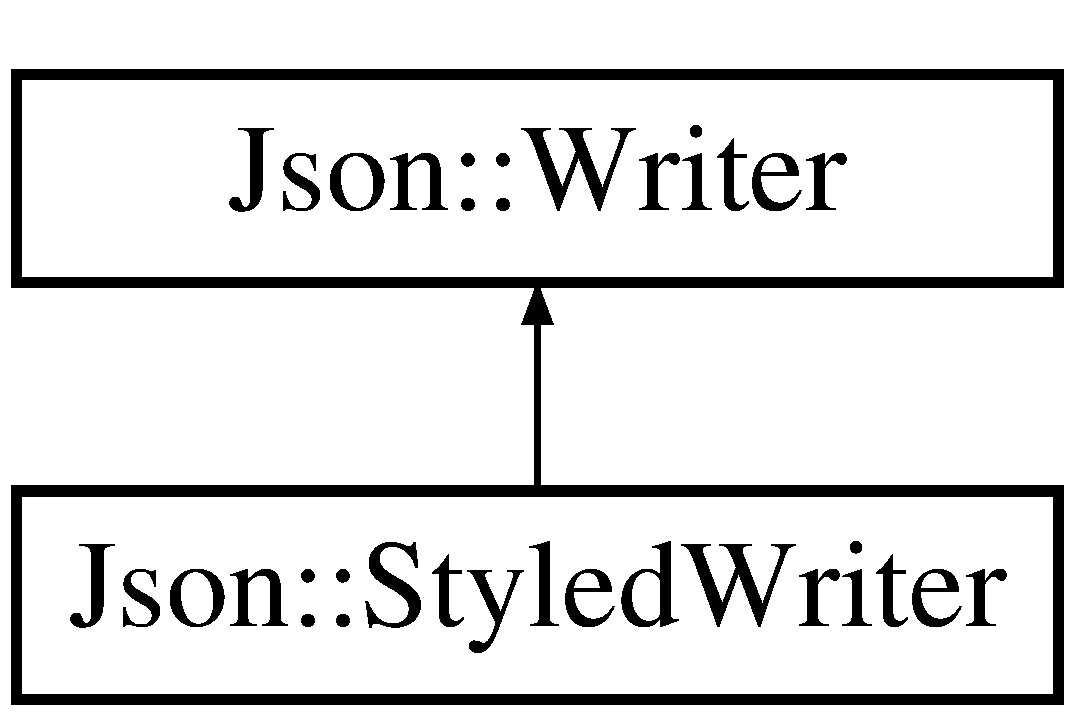
\includegraphics[height=2.000000cm]{class_json_1_1_styled_writer}
\end{center}
\end{figure}
\subsection*{Public Member Functions}
\begin{DoxyCompactItemize}
\item 
std\+::string \hyperlink{class_json_1_1_styled_writer_a56f0fd80f60272b3f3c85690aae66e7d}{write} (const \hyperlink{class_json_1_1_value}{Value} \&root)
\begin{DoxyCompactList}\small\item\em Serialize a \hyperlink{class_json_1_1_value}{Value} in \href{http://www.json.org}{\tt J\+S\+O\+N} format. \end{DoxyCompactList}\end{DoxyCompactItemize}
\subsection*{Private Types}
\begin{DoxyCompactItemize}
\item 
\hypertarget{class_json_1_1_styled_writer_a0b102abcd4b7e11eb22df63921e097df}{}typedef std\+::vector$<$ std\+::string $>$ {\bfseries Child\+Values}\label{class_json_1_1_styled_writer_a0b102abcd4b7e11eb22df63921e097df}

\end{DoxyCompactItemize}
\subsection*{Private Member Functions}
\begin{DoxyCompactItemize}
\item 
\hypertarget{class_json_1_1_styled_writer_ac40143cf43f7c4a94d3d0b41e5245069}{}void {\bfseries write\+Value} (const \hyperlink{class_json_1_1_value}{Value} \&value)\label{class_json_1_1_styled_writer_ac40143cf43f7c4a94d3d0b41e5245069}

\item 
\hypertarget{class_json_1_1_styled_writer_a0618c23d62965515def15ece1e677f5d}{}void {\bfseries write\+Array\+Value} (const \hyperlink{class_json_1_1_value}{Value} \&value)\label{class_json_1_1_styled_writer_a0618c23d62965515def15ece1e677f5d}

\item 
\hypertarget{class_json_1_1_styled_writer_aa5dc671edf10b9976f1511da2271ab9d}{}bool {\bfseries is\+Multine\+Array} (const \hyperlink{class_json_1_1_value}{Value} \&value)\label{class_json_1_1_styled_writer_aa5dc671edf10b9976f1511da2271ab9d}

\item 
\hypertarget{class_json_1_1_styled_writer_aba120a1ff1b84411b32039188e8fb49f}{}void {\bfseries push\+Value} (const std\+::string \&value)\label{class_json_1_1_styled_writer_aba120a1ff1b84411b32039188e8fb49f}

\item 
\hypertarget{class_json_1_1_styled_writer_a885f4bfb5701896d60eee6716d2db7e4}{}void {\bfseries write\+Indent} ()\label{class_json_1_1_styled_writer_a885f4bfb5701896d60eee6716d2db7e4}

\item 
\hypertarget{class_json_1_1_styled_writer_a7b3cc9da3cb455ee9b2752307ac21b58}{}void {\bfseries write\+With\+Indent} (const std\+::string \&value)\label{class_json_1_1_styled_writer_a7b3cc9da3cb455ee9b2752307ac21b58}

\item 
\hypertarget{class_json_1_1_styled_writer_a0b65be6186a7c6638270990265e42b97}{}void {\bfseries indent} ()\label{class_json_1_1_styled_writer_a0b65be6186a7c6638270990265e42b97}

\item 
\hypertarget{class_json_1_1_styled_writer_acee1c9285519b573cfcb00b7e7f5a809}{}void {\bfseries unindent} ()\label{class_json_1_1_styled_writer_acee1c9285519b573cfcb00b7e7f5a809}

\item 
\hypertarget{class_json_1_1_styled_writer_ad3452c48fabf968bf3693549331ec06e}{}void {\bfseries write\+Comment\+Before\+Value} (const \hyperlink{class_json_1_1_value}{Value} \&root)\label{class_json_1_1_styled_writer_ad3452c48fabf968bf3693549331ec06e}

\item 
\hypertarget{class_json_1_1_styled_writer_ab12b274c62822fc51ec4617c6be95139}{}void {\bfseries write\+Comment\+After\+Value\+On\+Same\+Line} (const \hyperlink{class_json_1_1_value}{Value} \&root)\label{class_json_1_1_styled_writer_ab12b274c62822fc51ec4617c6be95139}

\item 
\hypertarget{class_json_1_1_styled_writer_a37a806d010f708cb68556f2666f79bdf}{}bool {\bfseries has\+Comment\+For\+Value} (const \hyperlink{class_json_1_1_value}{Value} \&value)\label{class_json_1_1_styled_writer_a37a806d010f708cb68556f2666f79bdf}

\end{DoxyCompactItemize}
\subsection*{Static Private Member Functions}
\begin{DoxyCompactItemize}
\item 
\hypertarget{class_json_1_1_styled_writer_ad9444449eecf1581f7d227a0b50ecc4d}{}static std\+::string {\bfseries normalize\+E\+O\+L} (const std\+::string \&text)\label{class_json_1_1_styled_writer_ad9444449eecf1581f7d227a0b50ecc4d}

\end{DoxyCompactItemize}
\subsection*{Private Attributes}
\begin{DoxyCompactItemize}
\item 
\hypertarget{class_json_1_1_styled_writer_a1f905495f0705365af117ec541e29fdf}{}Child\+Values {\bfseries child\+Values\+\_\+}\label{class_json_1_1_styled_writer_a1f905495f0705365af117ec541e29fdf}

\item 
\hypertarget{class_json_1_1_styled_writer_ac092c93313e7ab202b13e075d682faea}{}std\+::string {\bfseries document\+\_\+}\label{class_json_1_1_styled_writer_ac092c93313e7ab202b13e075d682faea}

\item 
\hypertarget{class_json_1_1_styled_writer_a98a33f1d4c853a4dbf87ca17499c5830}{}std\+::string {\bfseries indent\+String\+\_\+}\label{class_json_1_1_styled_writer_a98a33f1d4c853a4dbf87ca17499c5830}

\item 
\hypertarget{class_json_1_1_styled_writer_a9c8fc62cb4f3b4a6dbed470fea2aa567}{}int {\bfseries right\+Margin\+\_\+}\label{class_json_1_1_styled_writer_a9c8fc62cb4f3b4a6dbed470fea2aa567}

\item 
\hypertarget{class_json_1_1_styled_writer_ae911f06042935286c24a9fb23dba78bd}{}int {\bfseries indent\+Size\+\_\+}\label{class_json_1_1_styled_writer_ae911f06042935286c24a9fb23dba78bd}

\item 
\hypertarget{class_json_1_1_styled_writer_acaabfa48b50a8bb7fa9ce98e2ae971d9}{}bool {\bfseries add\+Child\+Values\+\_\+}\label{class_json_1_1_styled_writer_acaabfa48b50a8bb7fa9ce98e2ae971d9}

\end{DoxyCompactItemize}


\subsection{Detailed Description}
Writes a \hyperlink{class_json_1_1_value}{Value} in \href{http://www.json.org}{\tt J\+S\+O\+N} format in a human friendly way. 

The rules for line break and indent are as follow\+:
\begin{DoxyItemize}
\item Object value\+:
\begin{DoxyItemize}
\item if empty then print \{\} without indent and line break
\item if not empty the print \textquotesingle{}\{\textquotesingle{}, line break \& indent, print one value per line and then unindent and line break and print \textquotesingle{}\}\textquotesingle{}.
\end{DoxyItemize}
\item Array value\+:
\begin{DoxyItemize}
\item if empty then print \mbox{[}\mbox{]} without indent and line break
\item if the array contains no object value, empty array or some other value types, and all the values fit on one lines, then print the array on a single line.
\item otherwise, it the values do not fit on one line, or the array contains object or non empty array, then print one value per line.
\end{DoxyItemize}
\end{DoxyItemize}

If the \hyperlink{class_json_1_1_value}{Value} have comments then they are outputed according to their \hyperlink{namespace_json_a4fc417c23905b2ae9e2c47d197a45351}{Comment\+Placement}.

\begin{DoxySeeAlso}{See also}
\hyperlink{class_json_1_1_reader}{Reader}, \hyperlink{class_json_1_1_value}{Value}, \hyperlink{class_json_1_1_value_a29f3a30f7e5d3af6f38d57999bf5b480}{Value\+::set\+Comment()} 
\end{DoxySeeAlso}
\begin{DoxyRefDesc}{Deprecated}
\item[\hyperlink{deprecated__deprecated000009}{Deprecated}]Use \hyperlink{class_json_1_1_stream_writer_builder}{Stream\+Writer\+Builder}. \end{DoxyRefDesc}


\subsection{Member Function Documentation}
\hypertarget{class_json_1_1_styled_writer_a56f0fd80f60272b3f3c85690aae66e7d}{}\index{Json\+::\+Styled\+Writer@{Json\+::\+Styled\+Writer}!write@{write}}
\index{write@{write}!Json\+::\+Styled\+Writer@{Json\+::\+Styled\+Writer}}
\subsubsection[{write(const Value \&root)}]{\setlength{\rightskip}{0pt plus 5cm}std\+::string Json\+::\+Styled\+Writer\+::write (
\begin{DoxyParamCaption}
\item[{const {\bf Value} \&}]{root}
\end{DoxyParamCaption}
)\hspace{0.3cm}{\ttfamily [virtual]}}\label{class_json_1_1_styled_writer_a56f0fd80f60272b3f3c85690aae66e7d}


Serialize a \hyperlink{class_json_1_1_value}{Value} in \href{http://www.json.org}{\tt J\+S\+O\+N} format. 


\begin{DoxyParams}{Parameters}
{\em root} & \hyperlink{class_json_1_1_value}{Value} to serialize. \\
\hline
\end{DoxyParams}
\begin{DoxyReturn}{Returns}
String containing the J\+S\+O\+N document that represents the root value. 
\end{DoxyReturn}


Implements \hyperlink{class_json_1_1_writer}{Json\+::\+Writer}.



The documentation for this class was generated from the following files\+:\begin{DoxyCompactItemize}
\item 
C\+:/\+Users/\+Mook T/\+Desktop/item/json.\+h\item 
C\+:/\+Users/\+Mook T/\+Desktop/item/jsoncpp.\+cpp\end{DoxyCompactItemize}

\hypertarget{class_json_1_1_reader_1_1_token}{}\section{Json\+:\+:Reader\+:\+:Token Class Reference}
\label{class_json_1_1_reader_1_1_token}\index{Json\+::\+Reader\+::\+Token@{Json\+::\+Reader\+::\+Token}}
\subsection*{Public Attributes}
\begin{DoxyCompactItemize}
\item 
\hypertarget{class_json_1_1_reader_1_1_token_aa0f06d0105ec3d8cb42427c66b991bad}{}Token\+Type {\bfseries type\+\_\+}\label{class_json_1_1_reader_1_1_token_aa0f06d0105ec3d8cb42427c66b991bad}

\item 
\hypertarget{class_json_1_1_reader_1_1_token_aff87d677b9ac4b52542a00b0d6673249}{}Location {\bfseries start\+\_\+}\label{class_json_1_1_reader_1_1_token_aff87d677b9ac4b52542a00b0d6673249}

\item 
\hypertarget{class_json_1_1_reader_1_1_token_a7d3bc0fa40097f435d184be4b1fd5ae1}{}Location {\bfseries end\+\_\+}\label{class_json_1_1_reader_1_1_token_a7d3bc0fa40097f435d184be4b1fd5ae1}

\end{DoxyCompactItemize}


The documentation for this class was generated from the following file\+:\begin{DoxyCompactItemize}
\item 
C\+:/\+Users/\+Mook T/\+Desktop/item/json.\+h\end{DoxyCompactItemize}

\hypertarget{class_json_1_1_our_reader_1_1_token}{}\section{Json\+:\+:Our\+Reader\+:\+:Token Class Reference}
\label{class_json_1_1_our_reader_1_1_token}\index{Json\+::\+Our\+Reader\+::\+Token@{Json\+::\+Our\+Reader\+::\+Token}}
\subsection*{Public Attributes}
\begin{DoxyCompactItemize}
\item 
\hypertarget{class_json_1_1_our_reader_1_1_token_abe7d858530396fa7e1293f7a579880ed}{}Token\+Type {\bfseries type\+\_\+}\label{class_json_1_1_our_reader_1_1_token_abe7d858530396fa7e1293f7a579880ed}

\item 
\hypertarget{class_json_1_1_our_reader_1_1_token_aedf68bb00eaaa9d3c22b9825999602ac}{}Location {\bfseries start\+\_\+}\label{class_json_1_1_our_reader_1_1_token_aedf68bb00eaaa9d3c22b9825999602ac}

\item 
\hypertarget{class_json_1_1_our_reader_1_1_token_a67d2071638add857528579ae3791eccc}{}Location {\bfseries end\+\_\+}\label{class_json_1_1_our_reader_1_1_token_a67d2071638add857528579ae3791eccc}

\end{DoxyCompactItemize}


The documentation for this class was generated from the following file\+:\begin{DoxyCompactItemize}
\item 
C\+:/\+Users/\+Mook T/\+Desktop/item/jsoncpp.\+cpp\end{DoxyCompactItemize}

\hypertarget{class_json_1_1_value}{}\section{Json\+:\+:Value Class Reference}
\label{class_json_1_1_value}\index{Json\+::\+Value@{Json\+::\+Value}}


Represents a \href{http://www.json.org}{\tt J\+S\+O\+N} value.  




{\ttfamily \#include $<$json.\+h$>$}

\subsection*{Classes}
\begin{DoxyCompactItemize}
\item 
struct \hyperlink{struct_json_1_1_value_1_1_comment_info}{Comment\+Info}
\item 
class \hyperlink{class_json_1_1_value_1_1_c_z_string}{C\+Z\+String}
\item 
union \hyperlink{union_json_1_1_value_1_1_value_holder}{Value\+Holder}
\end{DoxyCompactItemize}
\subsection*{Public Types}
\begin{DoxyCompactItemize}
\item 
\hypertarget{class_json_1_1_value_ac61bab5a465848b57610379cc07995c3}{}typedef std\+::vector$<$ std\+::string $>$ {\bfseries Members}\label{class_json_1_1_value_ac61bab5a465848b57610379cc07995c3}

\item 
\hypertarget{class_json_1_1_value_a341cdf2e01f8b3c5b7317aa2f0768c53}{}typedef \hyperlink{class_json_1_1_value_iterator}{Value\+Iterator} {\bfseries iterator}\label{class_json_1_1_value_a341cdf2e01f8b3c5b7317aa2f0768c53}

\item 
\hypertarget{class_json_1_1_value_af92282ca92b58b320debd486afb7696a}{}typedef \hyperlink{class_json_1_1_value_const_iterator}{Value\+Const\+Iterator} {\bfseries const\+\_\+iterator}\label{class_json_1_1_value_af92282ca92b58b320debd486afb7696a}

\item 
\hypertarget{class_json_1_1_value_a0933d59b45793ae4aade1757c322a98d}{}typedef Json\+::\+U\+Int {\bfseries U\+Int}\label{class_json_1_1_value_a0933d59b45793ae4aade1757c322a98d}

\item 
\hypertarget{class_json_1_1_value_abdf7a7ff73eb130ffcab28504ffdb405}{}typedef Json\+::\+Int {\bfseries Int}\label{class_json_1_1_value_abdf7a7ff73eb130ffcab28504ffdb405}

\item 
\hypertarget{class_json_1_1_value_a8b62564be8c087c6d18de180ff4e13e3}{}typedef Json\+::\+U\+Int64 {\bfseries U\+Int64}\label{class_json_1_1_value_a8b62564be8c087c6d18de180ff4e13e3}

\item 
\hypertarget{class_json_1_1_value_a1b86af9f85f0f1baa972c3319fa22695}{}typedef Json\+::\+Int64 {\bfseries Int64}\label{class_json_1_1_value_a1b86af9f85f0f1baa972c3319fa22695}

\item 
\hypertarget{class_json_1_1_value_a1cbb82642ed05109b9833e49f042ece7}{}typedef Json\+::\+Largest\+Int {\bfseries Largest\+Int}\label{class_json_1_1_value_a1cbb82642ed05109b9833e49f042ece7}

\item 
\hypertarget{class_json_1_1_value_a6682a3684d635e03fc06ba229fa24eec}{}typedef Json\+::\+Largest\+U\+Int {\bfseries Largest\+U\+Int}\label{class_json_1_1_value_a6682a3684d635e03fc06ba229fa24eec}

\item 
\hypertarget{class_json_1_1_value_a184a91566cccca7b819240f0d5561c7d}{}typedef Json\+::\+Array\+Index {\bfseries Array\+Index}\label{class_json_1_1_value_a184a91566cccca7b819240f0d5561c7d}

\item 
\hypertarget{class_json_1_1_value_a08b6c80c3af7071d908dabf044de5388}{}typedef std\+::map$<$ \hyperlink{class_json_1_1_value_1_1_c_z_string}{C\+Z\+String}, \hyperlink{class_json_1_1_value}{Value} $>$ {\bfseries Object\+Values}\label{class_json_1_1_value_a08b6c80c3af7071d908dabf044de5388}

\end{DoxyCompactItemize}
\subsection*{Public Member Functions}
\begin{DoxyCompactItemize}
\item 
\hyperlink{class_json_1_1_value_ada6ba1369448fb0240bccc36efaa46f7}{Value} (\hyperlink{namespace_json_a7d654b75c16a57007925868e38212b4e}{Value\+Type} type=\hyperlink{namespace_json_a7d654b75c16a57007925868e38212b4ea7d9899633b4409bd3fc107e6737f8391}{null\+Value})
\begin{DoxyCompactList}\small\item\em Create a default \hyperlink{class_json_1_1_value}{Value} of the given type. \end{DoxyCompactList}\item 
\hypertarget{class_json_1_1_value_a4744ae571fcf34f4b16a2257b3b3b585}{}{\bfseries Value} (Int value)\label{class_json_1_1_value_a4744ae571fcf34f4b16a2257b3b3b585}

\item 
\hypertarget{class_json_1_1_value_ae67a857b01286e3499a87e95be848d20}{}{\bfseries Value} (U\+Int value)\label{class_json_1_1_value_ae67a857b01286e3499a87e95be848d20}

\item 
\hypertarget{class_json_1_1_value_ab1cdc3d9a4d4cc03fa01439d43ceb1b5}{}{\bfseries Value} (Int64 value)\label{class_json_1_1_value_ab1cdc3d9a4d4cc03fa01439d43ceb1b5}

\item 
\hypertarget{class_json_1_1_value_a8adda58d5ae17bf7ca6a53bab4a7b69c}{}{\bfseries Value} (U\+Int64 value)\label{class_json_1_1_value_a8adda58d5ae17bf7ca6a53bab4a7b69c}

\item 
\hypertarget{class_json_1_1_value_a32228cc84d83200cca8441451997996c}{}{\bfseries Value} (double value)\label{class_json_1_1_value_a32228cc84d83200cca8441451997996c}

\item 
\hypertarget{class_json_1_1_value_ad87b849356816aca75995dd07302e49d}{}\hyperlink{class_json_1_1_value_ad87b849356816aca75995dd07302e49d}{Value} (const char $\ast$value)\label{class_json_1_1_value_ad87b849356816aca75995dd07302e49d}

\begin{DoxyCompactList}\small\item\em Copy til first 0. (N\+U\+L\+L causes to seg-\/fault.) \end{DoxyCompactList}\item 
\hypertarget{class_json_1_1_value_a39fa09d1902efbd4350e1236db920571}{}\hyperlink{class_json_1_1_value_a39fa09d1902efbd4350e1236db920571}{Value} (const char $\ast$begin, const char $\ast$end)\label{class_json_1_1_value_a39fa09d1902efbd4350e1236db920571}

\begin{DoxyCompactList}\small\item\em Copy all, incl zeroes. \end{DoxyCompactList}\item 
\hyperlink{class_json_1_1_value_a081830e95f88a37054da7e46c65b0766}{Value} (const \hyperlink{class_json_1_1_static_string}{Static\+String} \&value)
\begin{DoxyCompactList}\small\item\em Constructs a value from a static string. \end{DoxyCompactList}\item 
\hypertarget{class_json_1_1_value_aa4501dd4edf3ce3d5145fc656f088b21}{}\hyperlink{class_json_1_1_value_aa4501dd4edf3ce3d5145fc656f088b21}{Value} (const std\+::string \&value)\label{class_json_1_1_value_aa4501dd4edf3ce3d5145fc656f088b21}

\begin{DoxyCompactList}\small\item\em Copy data() til \hyperlink{class_json_1_1_value_a4ca8ee6c48a34ca6c2f131956bab5e05}{size()}. Embedded zeroes too. \end{DoxyCompactList}\item 
\hypertarget{class_json_1_1_value_a350a31ea4a30d384994b0bc010b17495}{}{\bfseries Value} (bool value)\label{class_json_1_1_value_a350a31ea4a30d384994b0bc010b17495}

\item 
\hypertarget{class_json_1_1_value_a436dfd3670f95fd665f680eba5cebcf0}{}\hyperlink{class_json_1_1_value_a436dfd3670f95fd665f680eba5cebcf0}{Value} (const \hyperlink{class_json_1_1_value}{Value} \&other)\label{class_json_1_1_value_a436dfd3670f95fd665f680eba5cebcf0}

\begin{DoxyCompactList}\small\item\em Deep copy. \end{DoxyCompactList}\item 
\hyperlink{class_json_1_1_value}{Value} \& \hyperlink{class_json_1_1_value_a795acb28772da4c5d85ae8f4af36c69f}{operator=} (\hyperlink{class_json_1_1_value}{Value} other)
\item 
\hypertarget{class_json_1_1_value_aab841120d78e296e1bc06a373345e822}{}void \hyperlink{class_json_1_1_value_aab841120d78e296e1bc06a373345e822}{swap} (\hyperlink{class_json_1_1_value}{Value} \&other)\label{class_json_1_1_value_aab841120d78e296e1bc06a373345e822}

\begin{DoxyCompactList}\small\item\em Swap everything. \end{DoxyCompactList}\item 
\hypertarget{class_json_1_1_value_a5263476047f20e2fc6de470e4de34fe5}{}void \hyperlink{class_json_1_1_value_a5263476047f20e2fc6de470e4de34fe5}{swap\+Payload} (\hyperlink{class_json_1_1_value}{Value} \&other)\label{class_json_1_1_value_a5263476047f20e2fc6de470e4de34fe5}

\begin{DoxyCompactList}\small\item\em Swap values but leave comments and source offsets in place. \end{DoxyCompactList}\item 
\hypertarget{class_json_1_1_value_a695ef31fad36b4712918b3ff80158479}{}\hyperlink{namespace_json_a7d654b75c16a57007925868e38212b4e}{Value\+Type} {\bfseries type} () const \label{class_json_1_1_value_a695ef31fad36b4712918b3ff80158479}

\item 
\hypertarget{class_json_1_1_value_af0ad8aa027575c3277296458f3fb7b0a}{}bool \hyperlink{class_json_1_1_value_af0ad8aa027575c3277296458f3fb7b0a}{operator$<$} (const \hyperlink{class_json_1_1_value}{Value} \&other) const \label{class_json_1_1_value_af0ad8aa027575c3277296458f3fb7b0a}

\begin{DoxyCompactList}\small\item\em Compare payload only, not comments etc. \end{DoxyCompactList}\item 
\hypertarget{class_json_1_1_value_afb99dd3628fe44244b32007f9b4f369a}{}bool {\bfseries operator$<$=} (const \hyperlink{class_json_1_1_value}{Value} \&other) const \label{class_json_1_1_value_afb99dd3628fe44244b32007f9b4f369a}

\item 
\hypertarget{class_json_1_1_value_acc13fc47d55abd6e2327b090b83d2911}{}bool {\bfseries operator$>$=} (const \hyperlink{class_json_1_1_value}{Value} \&other) const \label{class_json_1_1_value_acc13fc47d55abd6e2327b090b83d2911}

\item 
\hypertarget{class_json_1_1_value_a3124a26067bdfde9571bc89527fc6931}{}bool {\bfseries operator$>$} (const \hyperlink{class_json_1_1_value}{Value} \&other) const \label{class_json_1_1_value_a3124a26067bdfde9571bc89527fc6931}

\item 
\hypertarget{class_json_1_1_value_a14363dda23a6ae2def9afd1590ae85d3}{}bool {\bfseries operator==} (const \hyperlink{class_json_1_1_value}{Value} \&other) const \label{class_json_1_1_value_a14363dda23a6ae2def9afd1590ae85d3}

\item 
\hypertarget{class_json_1_1_value_ad0f12d2a4ab74bbef08a05504b2cb81d}{}bool {\bfseries operator!=} (const \hyperlink{class_json_1_1_value}{Value} \&other) const \label{class_json_1_1_value_ad0f12d2a4ab74bbef08a05504b2cb81d}

\item 
\hypertarget{class_json_1_1_value_a899214ed2253d3f4f061b922b0e622b5}{}int {\bfseries compare} (const \hyperlink{class_json_1_1_value}{Value} \&other) const \label{class_json_1_1_value_a899214ed2253d3f4f061b922b0e622b5}

\item 
\hypertarget{class_json_1_1_value_a5b7da48b163bcec63b1424f1608b7da6}{}const char $\ast$ \hyperlink{class_json_1_1_value_a5b7da48b163bcec63b1424f1608b7da6}{as\+C\+String} () const \label{class_json_1_1_value_a5b7da48b163bcec63b1424f1608b7da6}

\begin{DoxyCompactList}\small\item\em Embedded zeroes could cause you trouble! \end{DoxyCompactList}\item 
\hypertarget{class_json_1_1_value_a03ee3d5df576640c93ba683f140828bd}{}std\+::string \hyperlink{class_json_1_1_value_a03ee3d5df576640c93ba683f140828bd}{as\+String} () const \label{class_json_1_1_value_a03ee3d5df576640c93ba683f140828bd}

\begin{DoxyCompactList}\small\item\em Embedded zeroes are possible. \end{DoxyCompactList}\item 
bool \hyperlink{class_json_1_1_value_a1e0263113ae247a632afac43ebc4149f}{get\+String} (char const $\ast$$\ast$begin, char const $\ast$$\ast$end) const 
\item 
\hypertarget{class_json_1_1_value_ac786e35b860b1d700cb3d3e56dd6a235}{}Int {\bfseries as\+Int} () const \label{class_json_1_1_value_ac786e35b860b1d700cb3d3e56dd6a235}

\item 
\hypertarget{class_json_1_1_value_a2019d1bd296b89356c1b0da5970c918c}{}U\+Int {\bfseries as\+U\+Int} () const \label{class_json_1_1_value_a2019d1bd296b89356c1b0da5970c918c}

\item 
\hypertarget{class_json_1_1_value_a7f739b55aef060f4ab6360bfe1912b77}{}Int64 {\bfseries as\+Int64} () const \label{class_json_1_1_value_a7f739b55aef060f4ab6360bfe1912b77}

\item 
\hypertarget{class_json_1_1_value_a65acdab039f60ff0da15e622f2e17739}{}U\+Int64 {\bfseries as\+U\+Int64} () const \label{class_json_1_1_value_a65acdab039f60ff0da15e622f2e17739}

\item 
\hypertarget{class_json_1_1_value_a3786bb100c5cf9a98eb6d13784968956}{}Largest\+Int {\bfseries as\+Largest\+Int} () const \label{class_json_1_1_value_a3786bb100c5cf9a98eb6d13784968956}

\item 
\hypertarget{class_json_1_1_value_a692b88345a745b2f89ca5d94b52e94d4}{}Largest\+U\+Int {\bfseries as\+Largest\+U\+Int} () const \label{class_json_1_1_value_a692b88345a745b2f89ca5d94b52e94d4}

\item 
\hypertarget{class_json_1_1_value_ac2128d7080499daf8c5b1c71da243f63}{}float {\bfseries as\+Float} () const \label{class_json_1_1_value_ac2128d7080499daf8c5b1c71da243f63}

\item 
\hypertarget{class_json_1_1_value_a33434ed1c0217a34d04c95fa5342fd37}{}double {\bfseries as\+Double} () const \label{class_json_1_1_value_a33434ed1c0217a34d04c95fa5342fd37}

\item 
\hypertarget{class_json_1_1_value_a7402c797285c020566c3db5f8ae4e940}{}bool {\bfseries as\+Bool} () const \label{class_json_1_1_value_a7402c797285c020566c3db5f8ae4e940}

\item 
\hypertarget{class_json_1_1_value_aeb9ad8b1bb91bdd72203dc884b3f4362}{}bool {\bfseries is\+Null} () const \label{class_json_1_1_value_aeb9ad8b1bb91bdd72203dc884b3f4362}

\item 
\hypertarget{class_json_1_1_value_a3c3716cc7a0216cb1b654bb8f61c8d13}{}bool {\bfseries is\+Bool} () const \label{class_json_1_1_value_a3c3716cc7a0216cb1b654bb8f61c8d13}

\item 
\hypertarget{class_json_1_1_value_ab0df4746d6787d2ce1db1a156c118f14}{}bool {\bfseries is\+Int} () const \label{class_json_1_1_value_ab0df4746d6787d2ce1db1a156c118f14}

\item 
\hypertarget{class_json_1_1_value_aba89690e5fd72d0f7121a30013470423}{}bool {\bfseries is\+Int64} () const \label{class_json_1_1_value_aba89690e5fd72d0f7121a30013470423}

\item 
\hypertarget{class_json_1_1_value_ae814ca1796fe2d43ac09898b70213989}{}bool {\bfseries is\+U\+Int} () const \label{class_json_1_1_value_ae814ca1796fe2d43ac09898b70213989}

\item 
\hypertarget{class_json_1_1_value_aa35efece2a6cba4d988d7d5b54db2fb8}{}bool {\bfseries is\+U\+Int64} () const \label{class_json_1_1_value_aa35efece2a6cba4d988d7d5b54db2fb8}

\item 
\hypertarget{class_json_1_1_value_aec4f74ef7b776b1d9c8a10fc3bb4add5}{}bool {\bfseries is\+Integral} () const \label{class_json_1_1_value_aec4f74ef7b776b1d9c8a10fc3bb4add5}

\item 
\hypertarget{class_json_1_1_value_a0ea567fa51fc808851698bef59b43626}{}bool {\bfseries is\+Double} () const \label{class_json_1_1_value_a0ea567fa51fc808851698bef59b43626}

\item 
\hypertarget{class_json_1_1_value_a8ce848900e2e8fa23a41fcc2c1409fab}{}bool {\bfseries is\+Numeric} () const \label{class_json_1_1_value_a8ce848900e2e8fa23a41fcc2c1409fab}

\item 
\hypertarget{class_json_1_1_value_a06c01d7c1e8151a5844b595ab00f46c7}{}bool {\bfseries is\+String} () const \label{class_json_1_1_value_a06c01d7c1e8151a5844b595ab00f46c7}

\item 
\hypertarget{class_json_1_1_value_ac8c898f93543e55b67418f94bced20af}{}bool {\bfseries is\+Array} () const \label{class_json_1_1_value_ac8c898f93543e55b67418f94bced20af}

\item 
\hypertarget{class_json_1_1_value_a80cffaa0402b80317c0437216bbb6d92}{}bool {\bfseries is\+Object} () const \label{class_json_1_1_value_a80cffaa0402b80317c0437216bbb6d92}

\item 
\hypertarget{class_json_1_1_value_a7ec153803631a27abf58cba2bb1af70c}{}bool {\bfseries is\+Convertible\+To} (\hyperlink{namespace_json_a7d654b75c16a57007925868e38212b4e}{Value\+Type} other) const \label{class_json_1_1_value_a7ec153803631a27abf58cba2bb1af70c}

\item 
\hypertarget{class_json_1_1_value_a4ca8ee6c48a34ca6c2f131956bab5e05}{}Array\+Index \hyperlink{class_json_1_1_value_a4ca8ee6c48a34ca6c2f131956bab5e05}{size} () const \label{class_json_1_1_value_a4ca8ee6c48a34ca6c2f131956bab5e05}

\begin{DoxyCompactList}\small\item\em Number of values in array or object. \end{DoxyCompactList}\item 
\hypertarget{class_json_1_1_value_a99c42d3ff8495dad1e91b43e66553c36}{}bool \hyperlink{class_json_1_1_value_a99c42d3ff8495dad1e91b43e66553c36}{empty} () const \label{class_json_1_1_value_a99c42d3ff8495dad1e91b43e66553c36}

\begin{DoxyCompactList}\small\item\em Return true if empty array, empty object, or null; otherwise, false. \end{DoxyCompactList}\item 
\hypertarget{class_json_1_1_value_a021ab0d15a807fbe051446c9c545ab61}{}bool \hyperlink{class_json_1_1_value_a021ab0d15a807fbe051446c9c545ab61}{operator!} () const \label{class_json_1_1_value_a021ab0d15a807fbe051446c9c545ab61}

\begin{DoxyCompactList}\small\item\em Return is\+Null() \end{DoxyCompactList}\item 
void \hyperlink{class_json_1_1_value_a501a4d67e6c875255c2ecc03ccd2019b}{clear} ()
\item 
void \hyperlink{class_json_1_1_value_aa284353271ada427dbfa04a42f2be407}{resize} (Array\+Index \hyperlink{class_json_1_1_value_a4ca8ee6c48a34ca6c2f131956bab5e05}{size})
\item 
\hyperlink{class_json_1_1_value}{Value} \& \hyperlink{class_json_1_1_value_a7d99f5dba388cdaa152ce6ef933d64ef}{operator\mbox{[}$\,$\mbox{]}} (Array\+Index index)
\item 
\hyperlink{class_json_1_1_value}{Value} \& \hyperlink{class_json_1_1_value_ac9182982c361e0ab621134d406e5f250}{operator\mbox{[}$\,$\mbox{]}} (int index)
\item 
const \hyperlink{class_json_1_1_value}{Value} \& \hyperlink{class_json_1_1_value_af151919e8947c430e34bed2b0b128601}{operator\mbox{[}$\,$\mbox{]}} (Array\+Index index) const 
\item 
const \hyperlink{class_json_1_1_value}{Value} \& \hyperlink{class_json_1_1_value_af9e02b38f4e63e491c300c20b275bdd7}{operator\mbox{[}$\,$\mbox{]}} (int index) const 
\item 
\hyperlink{class_json_1_1_value}{Value} \hyperlink{class_json_1_1_value_a28282c9b76fa031eba7a1843c47c16fe}{get} (Array\+Index index, const \hyperlink{class_json_1_1_value}{Value} \&default\+Value) const 
\item 
\hypertarget{class_json_1_1_value_aaa82ebb4b730ea1567d310874f47d147}{}bool \hyperlink{class_json_1_1_value_aaa82ebb4b730ea1567d310874f47d147}{is\+Valid\+Index} (Array\+Index index) const \label{class_json_1_1_value_aaa82ebb4b730ea1567d310874f47d147}

\begin{DoxyCompactList}\small\item\em Return true if index $<$ \hyperlink{class_json_1_1_value_a4ca8ee6c48a34ca6c2f131956bab5e05}{size()}. \end{DoxyCompactList}\item 
\hyperlink{class_json_1_1_value}{Value} \& \hyperlink{class_json_1_1_value_a7e49ac977e4bcf59745a09d426669f75}{append} (const \hyperlink{class_json_1_1_value}{Value} \&value)
\begin{DoxyCompactList}\small\item\em Append value to array at the end. \end{DoxyCompactList}\item 
\hyperlink{class_json_1_1_value}{Value} \& \hyperlink{class_json_1_1_value_acb912f4ec40a25ea6eb387730885f3d9}{operator\mbox{[}$\,$\mbox{]}} (const char $\ast$key)
\item 
const \hyperlink{class_json_1_1_value}{Value} \& \hyperlink{class_json_1_1_value_ae5f73ffc7a039bca81b7ca771bc5db55}{operator\mbox{[}$\,$\mbox{]}} (const char $\ast$key) const 
\item 
\hyperlink{class_json_1_1_value}{Value} \& \hyperlink{class_json_1_1_value_ae511c7d46bf457412fb55c9471af9f50}{operator\mbox{[}$\,$\mbox{]}} (const std\+::string \&key)
\item 
const \hyperlink{class_json_1_1_value}{Value} \& \hyperlink{class_json_1_1_value_a3c53bfd2381d5a61036d7dc0b023d697}{operator\mbox{[}$\,$\mbox{]}} (const std\+::string \&key) const 
\item 
\hyperlink{class_json_1_1_value}{Value} \& \hyperlink{class_json_1_1_value_ac3763d7d315ca65dc188e273722f7955}{operator\mbox{[}$\,$\mbox{]}} (const \hyperlink{class_json_1_1_static_string}{Static\+String} \&key)
\begin{DoxyCompactList}\small\item\em Access an object value by name, create a null member if it does not exist. \end{DoxyCompactList}\item 
\hyperlink{class_json_1_1_value}{Value} \hyperlink{class_json_1_1_value_ab76b3323cde14c7db20676d07b260ce7}{get} (const char $\ast$key, const \hyperlink{class_json_1_1_value}{Value} \&default\+Value) const 
\item 
\hyperlink{class_json_1_1_value}{Value} \hyperlink{class_json_1_1_value_abcb2289c005bc0befdedaa94f662f63f}{get} (const char $\ast$begin, const char $\ast$end, const \hyperlink{class_json_1_1_value}{Value} \&default\+Value) const 
\item 
\hyperlink{class_json_1_1_value}{Value} \hyperlink{class_json_1_1_value_a54a34264356e01ee9c21a75ccfc809e9}{get} (const std\+::string \&key, const \hyperlink{class_json_1_1_value}{Value} \&default\+Value) const 
\item 
\hyperlink{class_json_1_1_value}{Value} const $\ast$ \hyperlink{class_json_1_1_value_a184bf49ec5da7ec31af089cf6f458f99}{find} (char const $\ast$begin, char const $\ast$end) const 
\item 
\hyperlink{class_json_1_1_value}{Value} const $\ast$ \hyperlink{class_json_1_1_value_afeb7ff596a0929d90c5f2f3cffb413ed}{demand} (char const $\ast$begin, char const $\ast$end)
\item 
\hyperlink{class_json_1_1_value}{Value} \hyperlink{class_json_1_1_value_aa52f7873b95d29627d6e83ba96f69aaa}{remove\+Member} (const char $\ast$key)
\begin{DoxyCompactList}\small\item\em Remove and return the named member. \end{DoxyCompactList}\item 
\hyperlink{class_json_1_1_value}{Value} \hyperlink{class_json_1_1_value_ae1f95f7ca3906e6bcc2a7be93210ecba}{remove\+Member} (const std\+::string \&key)
\item 
bool \hyperlink{class_json_1_1_value_a708e599489adf30d65bf85a8ee16e6fb}{remove\+Member} (const char $\ast$key, \hyperlink{class_json_1_1_value}{Value} $\ast$removed)
\item 
bool \hyperlink{class_json_1_1_value_a3749dae413a73eac05b7f8dc6deeb6a2}{remove\+Member} (std\+::string const \&key, \hyperlink{class_json_1_1_value}{Value} $\ast$removed)
\begin{DoxyCompactList}\small\item\em Remove the named map member. \end{DoxyCompactList}\item 
\hypertarget{class_json_1_1_value_a49c91af727d6b4eb0af02a81bb2def87}{}bool \hyperlink{class_json_1_1_value_a49c91af727d6b4eb0af02a81bb2def87}{remove\+Member} (const char $\ast$begin, const char $\ast$end, \hyperlink{class_json_1_1_value}{Value} $\ast$removed)\label{class_json_1_1_value_a49c91af727d6b4eb0af02a81bb2def87}

\begin{DoxyCompactList}\small\item\em Same as \hyperlink{class_json_1_1_value_a3749dae413a73eac05b7f8dc6deeb6a2}{remove\+Member(std\+::string const\& key, Value$\ast$ removed)} \end{DoxyCompactList}\item 
bool \hyperlink{class_json_1_1_value_ae9e67e08a85a2f3be3396ec0f4c47f65}{remove\+Index} (Array\+Index i, \hyperlink{class_json_1_1_value}{Value} $\ast$removed)
\begin{DoxyCompactList}\small\item\em Remove the indexed array element. \end{DoxyCompactList}\item 
bool \hyperlink{class_json_1_1_value_a196defba501d70ea2b6793afb04108e3}{is\+Member} (const char $\ast$key) const 
\item 
bool \hyperlink{class_json_1_1_value_af728b5738aaa133f3aad2e39dc4f415e}{is\+Member} (const std\+::string \&key) const 
\item 
\hypertarget{class_json_1_1_value_a077604b87a79d75543a1b5438eb9d8ab}{}bool \hyperlink{class_json_1_1_value_a077604b87a79d75543a1b5438eb9d8ab}{is\+Member} (const char $\ast$begin, const char $\ast$end) const \label{class_json_1_1_value_a077604b87a79d75543a1b5438eb9d8ab}

\begin{DoxyCompactList}\small\item\em Same as is\+Member(std\+::string const\& key)const. \end{DoxyCompactList}\item 
Members \hyperlink{class_json_1_1_value_a30fa08af88f2d0a038b22ba9f4e88b2a}{get\+Member\+Names} () const 
\begin{DoxyCompactList}\small\item\em Return a list of the member names. \end{DoxyCompactList}\item 
void \hyperlink{class_json_1_1_value_a29f3a30f7e5d3af6f38d57999bf5b480}{set\+Comment} (const char $\ast$comment, \hyperlink{namespace_json_a4fc417c23905b2ae9e2c47d197a45351}{Comment\+Placement} placement)
\item 
\hypertarget{class_json_1_1_value_a2900152a2887b410a9ddabe278b9d492}{}void \hyperlink{class_json_1_1_value_a2900152a2887b410a9ddabe278b9d492}{set\+Comment} (const char $\ast$comment, size\+\_\+t len, \hyperlink{namespace_json_a4fc417c23905b2ae9e2c47d197a45351}{Comment\+Placement} placement)\label{class_json_1_1_value_a2900152a2887b410a9ddabe278b9d492}

\begin{DoxyCompactList}\small\item\em Comments must be //... or /$\ast$ ... $\ast$/. \end{DoxyCompactList}\item 
\hypertarget{class_json_1_1_value_a6d68a2e7d4e1e317cd9e812e12181689}{}void \hyperlink{class_json_1_1_value_a6d68a2e7d4e1e317cd9e812e12181689}{set\+Comment} (const std\+::string \&comment, \hyperlink{namespace_json_a4fc417c23905b2ae9e2c47d197a45351}{Comment\+Placement} placement)\label{class_json_1_1_value_a6d68a2e7d4e1e317cd9e812e12181689}

\begin{DoxyCompactList}\small\item\em Comments must be //... or /$\ast$ ... $\ast$/. \end{DoxyCompactList}\item 
\hypertarget{class_json_1_1_value_a06567a00363cab9601be7e31336db03a}{}bool {\bfseries has\+Comment} (\hyperlink{namespace_json_a4fc417c23905b2ae9e2c47d197a45351}{Comment\+Placement} placement) const \label{class_json_1_1_value_a06567a00363cab9601be7e31336db03a}

\item 
\hypertarget{class_json_1_1_value_aa1e105b5d7f55d6e42f4fb2f3674116f}{}std\+::string \hyperlink{class_json_1_1_value_aa1e105b5d7f55d6e42f4fb2f3674116f}{get\+Comment} (\hyperlink{namespace_json_a4fc417c23905b2ae9e2c47d197a45351}{Comment\+Placement} placement) const \label{class_json_1_1_value_aa1e105b5d7f55d6e42f4fb2f3674116f}

\begin{DoxyCompactList}\small\item\em Include delimiters and embedded newlines. \end{DoxyCompactList}\item 
\hypertarget{class_json_1_1_value_a05357cf78959b790337fae4e5580ee4f}{}std\+::string {\bfseries to\+Styled\+String} () const \label{class_json_1_1_value_a05357cf78959b790337fae4e5580ee4f}

\item 
\hypertarget{class_json_1_1_value_ac12df0d6980600c5bac908ed0f64856e}{}\hyperlink{class_json_1_1_value_const_iterator}{const\+\_\+iterator} {\bfseries begin} () const \label{class_json_1_1_value_ac12df0d6980600c5bac908ed0f64856e}

\item 
\hypertarget{class_json_1_1_value_a596da1926b2f2a4056bff2edb713eb0b}{}\hyperlink{class_json_1_1_value_const_iterator}{const\+\_\+iterator} {\bfseries end} () const \label{class_json_1_1_value_a596da1926b2f2a4056bff2edb713eb0b}

\item 
\hypertarget{class_json_1_1_value_a2d45bb2e68e8f22fe356d7d955ebd3c9}{}\hyperlink{class_json_1_1_value_iterator}{iterator} {\bfseries begin} ()\label{class_json_1_1_value_a2d45bb2e68e8f22fe356d7d955ebd3c9}

\item 
\hypertarget{class_json_1_1_value_a2f961eff73f7f79cd29260b6cbd42558}{}\hyperlink{class_json_1_1_value_iterator}{iterator} {\bfseries end} ()\label{class_json_1_1_value_a2f961eff73f7f79cd29260b6cbd42558}

\item 
\hypertarget{class_json_1_1_value_a6d741407c3d784360c200f181b0d6d64}{}void {\bfseries set\+Offset\+Start} (size\+\_\+t start)\label{class_json_1_1_value_a6d741407c3d784360c200f181b0d6d64}

\item 
\hypertarget{class_json_1_1_value_ac6d858b5fd4d5fe6ca84f697def8c5ea}{}void {\bfseries set\+Offset\+Limit} (size\+\_\+t limit)\label{class_json_1_1_value_ac6d858b5fd4d5fe6ca84f697def8c5ea}

\item 
\hypertarget{class_json_1_1_value_a10142eda11ae0b1caecbcc9f436854d1}{}size\+\_\+t {\bfseries get\+Offset\+Start} () const \label{class_json_1_1_value_a10142eda11ae0b1caecbcc9f436854d1}

\item 
\hypertarget{class_json_1_1_value_acd7114469bc39368e9d93c29b54d8c8f}{}size\+\_\+t {\bfseries get\+Offset\+Limit} () const \label{class_json_1_1_value_acd7114469bc39368e9d93c29b54d8c8f}

\end{DoxyCompactItemize}
\subsection*{Static Public Attributes}
\begin{DoxyCompactItemize}
\item 
\hypertarget{class_json_1_1_value_a6d6e9ea6807e46d5b7ded66d3032f607}{}static const \hyperlink{class_json_1_1_value}{Value} \& \hyperlink{class_json_1_1_value_a6d6e9ea6807e46d5b7ded66d3032f607}{null} = reinterpret\+\_\+cast$<$const \hyperlink{class_json_1_1_value}{Value}\&$>$(k\+Null\+Ref)\label{class_json_1_1_value_a6d6e9ea6807e46d5b7ded66d3032f607}

\begin{DoxyCompactList}\small\item\em We regret this reference to a global instance; prefer the simpler \hyperlink{class_json_1_1_value_ada6ba1369448fb0240bccc36efaa46f7}{Value()}. \end{DoxyCompactList}\item 
static const \hyperlink{class_json_1_1_value}{Value} \& \hyperlink{class_json_1_1_value_aaa4ffd4e53967170c3e8c9abf682b5cd}{null\+Ref} = \hyperlink{class_json_1_1_value_a6d6e9ea6807e46d5b7ded66d3032f607}{null}
\item 
\hypertarget{class_json_1_1_value_af91df130daa50dd43d2cd89e6ee67706}{}static const Largest\+Int \hyperlink{class_json_1_1_value_af91df130daa50dd43d2cd89e6ee67706}{min\+Largest\+Int} = Largest\+Int($\sim$(Largest\+U\+Int(-\/1) / 2))\label{class_json_1_1_value_af91df130daa50dd43d2cd89e6ee67706}

\begin{DoxyCompactList}\small\item\em Minimum signed integer value that can be stored in a \hyperlink{class_json_1_1_value}{Json\+::\+Value}. \end{DoxyCompactList}\item 
\hypertarget{class_json_1_1_value_a8b4977696f13296fa8755c7953fafb2f}{}static const Largest\+Int \hyperlink{class_json_1_1_value_a8b4977696f13296fa8755c7953fafb2f}{max\+Largest\+Int} = Largest\+Int(Largest\+U\+Int(-\/1) / 2)\label{class_json_1_1_value_a8b4977696f13296fa8755c7953fafb2f}

\begin{DoxyCompactList}\small\item\em Maximum signed integer value that can be stored in a \hyperlink{class_json_1_1_value}{Json\+::\+Value}. \end{DoxyCompactList}\item 
\hypertarget{class_json_1_1_value_a8ddb32d9d55fa5323ae5135639dc2e31}{}static const Largest\+U\+Int \hyperlink{class_json_1_1_value_a8ddb32d9d55fa5323ae5135639dc2e31}{max\+Largest\+U\+Int} = Largest\+U\+Int(-\/1)\label{class_json_1_1_value_a8ddb32d9d55fa5323ae5135639dc2e31}

\begin{DoxyCompactList}\small\item\em Maximum unsigned integer value that can be stored in a \hyperlink{class_json_1_1_value}{Json\+::\+Value}. \end{DoxyCompactList}\item 
\hypertarget{class_json_1_1_value_a7df8a39e2502b8c92a6a41e3d752d2c8}{}static const Int \hyperlink{class_json_1_1_value_a7df8a39e2502b8c92a6a41e3d752d2c8}{min\+Int} = Int($\sim$(U\+Int(-\/1) / 2))\label{class_json_1_1_value_a7df8a39e2502b8c92a6a41e3d752d2c8}

\begin{DoxyCompactList}\small\item\em Minimum signed int value that can be stored in a \hyperlink{class_json_1_1_value}{Json\+::\+Value}. \end{DoxyCompactList}\item 
\hypertarget{class_json_1_1_value_a978c799a8af3114ef7dab6fd0a310a1b}{}static const Int \hyperlink{class_json_1_1_value_a978c799a8af3114ef7dab6fd0a310a1b}{max\+Int} = Int(U\+Int(-\/1) / 2)\label{class_json_1_1_value_a978c799a8af3114ef7dab6fd0a310a1b}

\begin{DoxyCompactList}\small\item\em Maximum signed int value that can be stored in a \hyperlink{class_json_1_1_value}{Json\+::\+Value}. \end{DoxyCompactList}\item 
\hypertarget{class_json_1_1_value_ac79e63ee68d3aa914bfd6988be669b87}{}static const U\+Int \hyperlink{class_json_1_1_value_ac79e63ee68d3aa914bfd6988be669b87}{max\+U\+Int} = U\+Int(-\/1)\label{class_json_1_1_value_ac79e63ee68d3aa914bfd6988be669b87}

\begin{DoxyCompactList}\small\item\em Maximum unsigned int value that can be stored in a \hyperlink{class_json_1_1_value}{Json\+::\+Value}. \end{DoxyCompactList}\item 
\hypertarget{class_json_1_1_value_a815ef899bc312c93bc426511acfe31a7}{}static const Int64 \hyperlink{class_json_1_1_value_a815ef899bc312c93bc426511acfe31a7}{min\+Int64} = Int64($\sim$(U\+Int64(-\/1) / 2))\label{class_json_1_1_value_a815ef899bc312c93bc426511acfe31a7}

\begin{DoxyCompactList}\small\item\em Minimum signed 64 bits int value that can be stored in a \hyperlink{class_json_1_1_value}{Json\+::\+Value}. \end{DoxyCompactList}\item 
\hypertarget{class_json_1_1_value_a4492634870b8c5709ce967b384ac6006}{}static const Int64 \hyperlink{class_json_1_1_value_a4492634870b8c5709ce967b384ac6006}{max\+Int64} = Int64(U\+Int64(-\/1) / 2)\label{class_json_1_1_value_a4492634870b8c5709ce967b384ac6006}

\begin{DoxyCompactList}\small\item\em Maximum signed 64 bits int value that can be stored in a \hyperlink{class_json_1_1_value}{Json\+::\+Value}. \end{DoxyCompactList}\item 
\hypertarget{class_json_1_1_value_ae1eb89c305c39516696ff305cffa01da}{}static const U\+Int64 \hyperlink{class_json_1_1_value_ae1eb89c305c39516696ff305cffa01da}{max\+U\+Int64} = U\+Int64(-\/1)\label{class_json_1_1_value_ae1eb89c305c39516696ff305cffa01da}

\begin{DoxyCompactList}\small\item\em Maximum unsigned 64 bits int value that can be stored in a \hyperlink{class_json_1_1_value}{Json\+::\+Value}. \end{DoxyCompactList}\end{DoxyCompactItemize}
\subsection*{Private Member Functions}
\begin{DoxyCompactItemize}
\item 
\hypertarget{class_json_1_1_value_a32b86b71564157f40f880f5736be822a}{}void {\bfseries init\+Basic} (\hyperlink{namespace_json_a7d654b75c16a57007925868e38212b4e}{Value\+Type} type, bool allocated=false)\label{class_json_1_1_value_a32b86b71564157f40f880f5736be822a}

\item 
\hypertarget{class_json_1_1_value_a9ff9cdae2c8f4155bab603d750b0b3f1}{}\hyperlink{class_json_1_1_value}{Value} \& {\bfseries resolve\+Reference} (const char $\ast$key)\label{class_json_1_1_value_a9ff9cdae2c8f4155bab603d750b0b3f1}

\item 
\hypertarget{class_json_1_1_value_a121c76136ac3255ad3de088b50652acb}{}\hyperlink{class_json_1_1_value}{Value} \& {\bfseries resolve\+Reference} (const char $\ast$key, const char $\ast$end)\label{class_json_1_1_value_a121c76136ac3255ad3de088b50652acb}

\end{DoxyCompactItemize}
\subsection*{Private Attributes}
\begin{DoxyCompactItemize}
\item 
\hypertarget{class_json_1_1_value_aef578244546212705b9f81eb84d7e151}{}union \hyperlink{union_json_1_1_value_1_1_value_holder}{Json\+::\+Value\+::\+Value\+Holder} {\bfseries value\+\_\+}\label{class_json_1_1_value_aef578244546212705b9f81eb84d7e151}

\item 
\hypertarget{class_json_1_1_value_abd222c2536dc88bf330dedcd076d2356}{}\hyperlink{namespace_json_a7d654b75c16a57007925868e38212b4e}{Value\+Type} {\bfseries type\+\_\+}\+: 8\label{class_json_1_1_value_abd222c2536dc88bf330dedcd076d2356}

\item 
\hypertarget{class_json_1_1_value_ae0126c80dc4907aad94088553fc7632b}{}unsigned int {\bfseries allocated\+\_\+}\+: 1\label{class_json_1_1_value_ae0126c80dc4907aad94088553fc7632b}

\item 
\hypertarget{class_json_1_1_value_a2016564cabc7a29208e97bd0b782a4e4}{}\hyperlink{struct_json_1_1_value_1_1_comment_info}{Comment\+Info} $\ast$ {\bfseries comments\+\_\+}\label{class_json_1_1_value_a2016564cabc7a29208e97bd0b782a4e4}

\item 
\hypertarget{class_json_1_1_value_a810637b8c52661a3dbf4bfde5130d6d1}{}size\+\_\+t {\bfseries start\+\_\+}\label{class_json_1_1_value_a810637b8c52661a3dbf4bfde5130d6d1}

\item 
\hypertarget{class_json_1_1_value_acbec44708b0d4dbec2db6d8428955dbb}{}size\+\_\+t {\bfseries limit\+\_\+}\label{class_json_1_1_value_acbec44708b0d4dbec2db6d8428955dbb}

\end{DoxyCompactItemize}
\subsection*{Friends}
\begin{DoxyCompactItemize}
\item 
\hypertarget{class_json_1_1_value_ad016df56489e5d360735457afba2f649}{}class {\bfseries Value\+Iterator\+Base}\label{class_json_1_1_value_ad016df56489e5d360735457afba2f649}

\end{DoxyCompactItemize}


\subsection{Detailed Description}
Represents a \href{http://www.json.org}{\tt J\+S\+O\+N} value. 

This class is a discriminated union wrapper that can represents a\+:
\begin{DoxyItemize}
\item signed integer \mbox{[}range\+: \hyperlink{class_json_1_1_value_a7df8a39e2502b8c92a6a41e3d752d2c8}{Value\+::min\+Int} -\/ \hyperlink{class_json_1_1_value_a978c799a8af3114ef7dab6fd0a310a1b}{Value\+::max\+Int}\mbox{]}
\item unsigned integer (range\+: 0 -\/ \hyperlink{class_json_1_1_value_ac79e63ee68d3aa914bfd6988be669b87}{Value\+::max\+U\+Int})
\item double
\item U\+T\+F-\/8 string
\item boolean
\item \textquotesingle{}null\textquotesingle{}
\item an ordered list of \hyperlink{class_json_1_1_value}{Value}
\item collection of name/value pairs (javascript object)
\end{DoxyItemize}

The type of the held value is represented by a \hyperlink{namespace_json_a7d654b75c16a57007925868e38212b4e}{Value\+Type} and can be obtained using type().

Values of an \hyperlink{namespace_json_a7d654b75c16a57007925868e38212b4eae8386dcfc36d1ae897745f7b4f77a1f6}{object\+Value} or \hyperlink{namespace_json_a7d654b75c16a57007925868e38212b4eadc8f264f36b55b063c78126b335415f4}{array\+Value} can be accessed using \hyperlink{class_json_1_1_value_a7d99f5dba388cdaa152ce6ef933d64ef}{operator\mbox{[}$\,$\mbox{]}()} methods. Non-\/const methods will automatically create the a \hyperlink{namespace_json_a7d654b75c16a57007925868e38212b4ea7d9899633b4409bd3fc107e6737f8391}{null\+Value} element if it does not exist. The sequence of an \hyperlink{namespace_json_a7d654b75c16a57007925868e38212b4eadc8f264f36b55b063c78126b335415f4}{array\+Value} will be automatically resized and initialized with \hyperlink{namespace_json_a7d654b75c16a57007925868e38212b4ea7d9899633b4409bd3fc107e6737f8391}{null\+Value}. \hyperlink{class_json_1_1_value_aa284353271ada427dbfa04a42f2be407}{resize()} can be used to enlarge or truncate an \hyperlink{namespace_json_a7d654b75c16a57007925868e38212b4eadc8f264f36b55b063c78126b335415f4}{array\+Value}.

The \hyperlink{class_json_1_1_value_a28282c9b76fa031eba7a1843c47c16fe}{get()} methods can be used to obtain default value in the case the required element does not exist.

It is possible to iterate over the list of a \hyperlink{namespace_json_a7d654b75c16a57007925868e38212b4eae8386dcfc36d1ae897745f7b4f77a1f6}{object\+Value} values using the \hyperlink{class_json_1_1_value_a30fa08af88f2d0a038b22ba9f4e88b2a}{get\+Member\+Names()} method.

\begin{DoxyNote}{Note}
\hyperlink{class_json_1_1_value_ada6ba1369448fb0240bccc36efaa46f7}{Value} string-\/length fit in size\+\_\+t, but keys must be $<$ 2$^\wedge$30. (The reason is an implementation detail.) A \#\+Char\+Reader will raise an exception if a bound is exceeded to avoid security holes in your app, but the \hyperlink{class_json_1_1_value}{Value} A\+P\+I does {\itshape not} check bounds. That is the responsibility of the caller. 
\end{DoxyNote}


\subsection{Constructor \& Destructor Documentation}
\hypertarget{class_json_1_1_value_ada6ba1369448fb0240bccc36efaa46f7}{}\index{Json\+::\+Value@{Json\+::\+Value}!Value@{Value}}
\index{Value@{Value}!Json\+::\+Value@{Json\+::\+Value}}
\subsubsection[{Value(\+Value\+Type type=null\+Value)}]{\setlength{\rightskip}{0pt plus 5cm}Json\+::\+Value\+::\+Value (
\begin{DoxyParamCaption}
\item[{{\bf Value\+Type}}]{type = {\ttfamily {\bf null\+Value}}}
\end{DoxyParamCaption}
)}\label{class_json_1_1_value_ada6ba1369448fb0240bccc36efaa46f7}


Create a default \hyperlink{class_json_1_1_value}{Value} of the given type. 

This is a very useful constructor. To create an empty array, pass array\+Value. To create an empty object, pass object\+Value. Another \hyperlink{class_json_1_1_value}{Value} can then be set to this one by assignment. This is useful since \hyperlink{class_json_1_1_value_a501a4d67e6c875255c2ecc03ccd2019b}{clear()} and \hyperlink{class_json_1_1_value_aa284353271ada427dbfa04a42f2be407}{resize()} will not alter types. \begin{DoxyVerb}Examples:
\end{DoxyVerb}
 
\begin{DoxyCode}
\hyperlink{class_json_1_1_value}{Json::Value} null\_value; \textcolor{comment}{// null}
\hyperlink{class_json_1_1_value}{Json::Value} arr\_value(\hyperlink{namespace_json_a7d654b75c16a57007925868e38212b4eadc8f264f36b55b063c78126b335415f4}{Json::arrayValue}); \textcolor{comment}{// []}
\hyperlink{class_json_1_1_value}{Json::Value} obj\_value(\hyperlink{namespace_json_a7d654b75c16a57007925868e38212b4eae8386dcfc36d1ae897745f7b4f77a1f6}{Json::objectValue}); \textcolor{comment}{// \{\}}
\end{DoxyCode}
 \hypertarget{class_json_1_1_value_a081830e95f88a37054da7e46c65b0766}{}\index{Json\+::\+Value@{Json\+::\+Value}!Value@{Value}}
\index{Value@{Value}!Json\+::\+Value@{Json\+::\+Value}}
\subsubsection[{Value(const Static\+String \&value)}]{\setlength{\rightskip}{0pt plus 5cm}Json\+::\+Value\+::\+Value (
\begin{DoxyParamCaption}
\item[{const {\bf Static\+String} \&}]{value}
\end{DoxyParamCaption}
)}\label{class_json_1_1_value_a081830e95f88a37054da7e46c65b0766}


Constructs a value from a static string. 

Like other value string constructor but do not duplicate the string for internal storage. The given string must remain alive after the call to this constructor. \begin{DoxyNote}{Note}
This works only for null-\/terminated strings. (We cannot change the size of this class, so we have nowhere to store the length, which might be computed later for various operations.)
\end{DoxyNote}
Example of usage\+: 
\begin{DoxyCode}
\textcolor{keyword}{static} StaticString foo(\textcolor{stringliteral}{"some text"});
\hyperlink{class_json_1_1_value}{Json::Value} aValue(foo);
\end{DoxyCode}
 

\subsection{Member Function Documentation}
\hypertarget{class_json_1_1_value_a7e49ac977e4bcf59745a09d426669f75}{}\index{Json\+::\+Value@{Json\+::\+Value}!append@{append}}
\index{append@{append}!Json\+::\+Value@{Json\+::\+Value}}
\subsubsection[{append(const Value \&value)}]{\setlength{\rightskip}{0pt plus 5cm}{\bf Value} \& Json\+::\+Value\+::append (
\begin{DoxyParamCaption}
\item[{const {\bf Value} \&}]{value}
\end{DoxyParamCaption}
)}\label{class_json_1_1_value_a7e49ac977e4bcf59745a09d426669f75}


Append value to array at the end. 

Equivalent to jsonvalue\mbox{[}jsonvalue.\+size()\mbox{]} = value; \hypertarget{class_json_1_1_value_a501a4d67e6c875255c2ecc03ccd2019b}{}\index{Json\+::\+Value@{Json\+::\+Value}!clear@{clear}}
\index{clear@{clear}!Json\+::\+Value@{Json\+::\+Value}}
\subsubsection[{clear()}]{\setlength{\rightskip}{0pt plus 5cm}void Json\+::\+Value\+::clear (
\begin{DoxyParamCaption}
{}
\end{DoxyParamCaption}
)}\label{class_json_1_1_value_a501a4d67e6c875255c2ecc03ccd2019b}
Remove all object members and array elements. \begin{DoxyPrecond}{Precondition}
type() is array\+Value, object\+Value, or null\+Value 
\end{DoxyPrecond}
\begin{DoxyPostcond}{Postcondition}
type() is unchanged 
\end{DoxyPostcond}
\hypertarget{class_json_1_1_value_afeb7ff596a0929d90c5f2f3cffb413ed}{}\index{Json\+::\+Value@{Json\+::\+Value}!demand@{demand}}
\index{demand@{demand}!Json\+::\+Value@{Json\+::\+Value}}
\subsubsection[{demand(char const $\ast$begin, char const $\ast$end)}]{\setlength{\rightskip}{0pt plus 5cm}{\bf Value} const$\ast$ Json\+::\+Value\+::demand (
\begin{DoxyParamCaption}
\item[{char const $\ast$}]{begin, }
\item[{char const $\ast$}]{end}
\end{DoxyParamCaption}
)}\label{class_json_1_1_value_afeb7ff596a0929d90c5f2f3cffb413ed}
Most general and efficient version of object-\/mutators. \begin{DoxyNote}{Note}
As stated elsewhere, behavior is undefined if (end-\/begin) $>$= 2$^\wedge$30 
\end{DoxyNote}
\begin{DoxyReturn}{Returns}
non-\/zero, but J\+S\+O\+N\+\_\+\+A\+S\+S\+E\+R\+T if this is neither object nor null\+Value. 
\end{DoxyReturn}
\hypertarget{class_json_1_1_value_a184bf49ec5da7ec31af089cf6f458f99}{}\index{Json\+::\+Value@{Json\+::\+Value}!find@{find}}
\index{find@{find}!Json\+::\+Value@{Json\+::\+Value}}
\subsubsection[{find(char const $\ast$begin, char const $\ast$end) const }]{\setlength{\rightskip}{0pt plus 5cm}{\bf Value} const $\ast$ Json\+::\+Value\+::find (
\begin{DoxyParamCaption}
\item[{char const $\ast$}]{begin, }
\item[{char const $\ast$}]{end}
\end{DoxyParamCaption}
) const}\label{class_json_1_1_value_a184bf49ec5da7ec31af089cf6f458f99}
Most general and efficient version of is\+Member()const, get()const, and operator\mbox{[}\mbox{]}const \begin{DoxyNote}{Note}
As stated elsewhere, behavior is undefined if (end-\/begin) $>$= 2$^\wedge$30 
\end{DoxyNote}
\hypertarget{class_json_1_1_value_a28282c9b76fa031eba7a1843c47c16fe}{}\index{Json\+::\+Value@{Json\+::\+Value}!get@{get}}
\index{get@{get}!Json\+::\+Value@{Json\+::\+Value}}
\subsubsection[{get(\+Array\+Index index, const Value \&default\+Value) const }]{\setlength{\rightskip}{0pt plus 5cm}{\bf Value} Json\+::\+Value\+::get (
\begin{DoxyParamCaption}
\item[{Array\+Index}]{index, }
\item[{const {\bf Value} \&}]{default\+Value}
\end{DoxyParamCaption}
) const}\label{class_json_1_1_value_a28282c9b76fa031eba7a1843c47c16fe}
If the array contains at least index+1 elements, returns the element value, otherwise returns default\+Value. \hypertarget{class_json_1_1_value_ab76b3323cde14c7db20676d07b260ce7}{}\index{Json\+::\+Value@{Json\+::\+Value}!get@{get}}
\index{get@{get}!Json\+::\+Value@{Json\+::\+Value}}
\subsubsection[{get(const char $\ast$key, const Value \&default\+Value) const }]{\setlength{\rightskip}{0pt plus 5cm}{\bf Value} Json\+::\+Value\+::get (
\begin{DoxyParamCaption}
\item[{const char $\ast$}]{key, }
\item[{const {\bf Value} \&}]{default\+Value}
\end{DoxyParamCaption}
) const}\label{class_json_1_1_value_ab76b3323cde14c7db20676d07b260ce7}
Return the member named key if it exist, default\+Value otherwise. \begin{DoxyNote}{Note}
deep copy 
\end{DoxyNote}
\hypertarget{class_json_1_1_value_abcb2289c005bc0befdedaa94f662f63f}{}\index{Json\+::\+Value@{Json\+::\+Value}!get@{get}}
\index{get@{get}!Json\+::\+Value@{Json\+::\+Value}}
\subsubsection[{get(const char $\ast$begin, const char $\ast$end, const Value \&default\+Value) const }]{\setlength{\rightskip}{0pt plus 5cm}{\bf Value} Json\+::\+Value\+::get (
\begin{DoxyParamCaption}
\item[{const char $\ast$}]{begin, }
\item[{const char $\ast$}]{end, }
\item[{const {\bf Value} \&}]{default\+Value}
\end{DoxyParamCaption}
) const}\label{class_json_1_1_value_abcb2289c005bc0befdedaa94f662f63f}
Return the member named key if it exist, default\+Value otherwise. \begin{DoxyNote}{Note}
deep copy 

key may contain embedded nulls. 
\end{DoxyNote}
\hypertarget{class_json_1_1_value_a54a34264356e01ee9c21a75ccfc809e9}{}\index{Json\+::\+Value@{Json\+::\+Value}!get@{get}}
\index{get@{get}!Json\+::\+Value@{Json\+::\+Value}}
\subsubsection[{get(const std\+::string \&key, const Value \&default\+Value) const }]{\setlength{\rightskip}{0pt plus 5cm}{\bf Value} Json\+::\+Value\+::get (
\begin{DoxyParamCaption}
\item[{const std\+::string \&}]{key, }
\item[{const {\bf Value} \&}]{default\+Value}
\end{DoxyParamCaption}
) const}\label{class_json_1_1_value_a54a34264356e01ee9c21a75ccfc809e9}
Return the member named key if it exist, default\+Value otherwise. \begin{DoxyNote}{Note}
deep copy 
\end{DoxyNote}

\begin{DoxyParams}{Parameters}
{\em key} & may contain embedded nulls. \\
\hline
\end{DoxyParams}
\hypertarget{class_json_1_1_value_a30fa08af88f2d0a038b22ba9f4e88b2a}{}\index{Json\+::\+Value@{Json\+::\+Value}!get\+Member\+Names@{get\+Member\+Names}}
\index{get\+Member\+Names@{get\+Member\+Names}!Json\+::\+Value@{Json\+::\+Value}}
\subsubsection[{get\+Member\+Names() const }]{\setlength{\rightskip}{0pt plus 5cm}Value\+::\+Members Json\+::\+Value\+::get\+Member\+Names (
\begin{DoxyParamCaption}
{}
\end{DoxyParamCaption}
) const}\label{class_json_1_1_value_a30fa08af88f2d0a038b22ba9f4e88b2a}


Return a list of the member names. 

If null, return an empty list. \begin{DoxyPrecond}{Precondition}
type() is object\+Value or null\+Value 
\end{DoxyPrecond}
\begin{DoxyPostcond}{Postcondition}
if type() was null\+Value, it remains null\+Value 
\end{DoxyPostcond}
\hypertarget{class_json_1_1_value_a1e0263113ae247a632afac43ebc4149f}{}\index{Json\+::\+Value@{Json\+::\+Value}!get\+String@{get\+String}}
\index{get\+String@{get\+String}!Json\+::\+Value@{Json\+::\+Value}}
\subsubsection[{get\+String(char const $\ast$$\ast$begin, char const $\ast$$\ast$end) const }]{\setlength{\rightskip}{0pt plus 5cm}bool Json\+::\+Value\+::get\+String (
\begin{DoxyParamCaption}
\item[{char const $\ast$$\ast$}]{begin, }
\item[{char const $\ast$$\ast$}]{end}
\end{DoxyParamCaption}
) const}\label{class_json_1_1_value_a1e0263113ae247a632afac43ebc4149f}
Get raw char$\ast$ of string-\/value. \begin{DoxyReturn}{Returns}
false if !string. (Seg-\/fault if str or end are N\+U\+L\+L.) 
\end{DoxyReturn}
\hypertarget{class_json_1_1_value_a196defba501d70ea2b6793afb04108e3}{}\index{Json\+::\+Value@{Json\+::\+Value}!is\+Member@{is\+Member}}
\index{is\+Member@{is\+Member}!Json\+::\+Value@{Json\+::\+Value}}
\subsubsection[{is\+Member(const char $\ast$key) const }]{\setlength{\rightskip}{0pt plus 5cm}bool Json\+::\+Value\+::is\+Member (
\begin{DoxyParamCaption}
\item[{const char $\ast$}]{key}
\end{DoxyParamCaption}
) const}\label{class_json_1_1_value_a196defba501d70ea2b6793afb04108e3}
Return true if the object has a member named key. \begin{DoxyNote}{Note}
\textquotesingle{}key\textquotesingle{} must be null-\/terminated. 
\end{DoxyNote}
\hypertarget{class_json_1_1_value_af728b5738aaa133f3aad2e39dc4f415e}{}\index{Json\+::\+Value@{Json\+::\+Value}!is\+Member@{is\+Member}}
\index{is\+Member@{is\+Member}!Json\+::\+Value@{Json\+::\+Value}}
\subsubsection[{is\+Member(const std\+::string \&key) const }]{\setlength{\rightskip}{0pt plus 5cm}bool Json\+::\+Value\+::is\+Member (
\begin{DoxyParamCaption}
\item[{const std\+::string \&}]{key}
\end{DoxyParamCaption}
) const}\label{class_json_1_1_value_af728b5738aaa133f3aad2e39dc4f415e}
Return true if the object has a member named key. 
\begin{DoxyParams}{Parameters}
{\em key} & may contain embedded nulls. \\
\hline
\end{DoxyParams}
\hypertarget{class_json_1_1_value_a795acb28772da4c5d85ae8f4af36c69f}{}\index{Json\+::\+Value@{Json\+::\+Value}!operator=@{operator=}}
\index{operator=@{operator=}!Json\+::\+Value@{Json\+::\+Value}}
\subsubsection[{operator=(\+Value other)}]{\setlength{\rightskip}{0pt plus 5cm}{\bf Value} \& Json\+::\+Value\+::operator= (
\begin{DoxyParamCaption}
\item[{{\bf Value}}]{other}
\end{DoxyParamCaption}
)}\label{class_json_1_1_value_a795acb28772da4c5d85ae8f4af36c69f}
Deep copy, then swap(other). \begin{DoxyNote}{Note}
Over-\/write existing comments. To preserve comments, use \hyperlink{class_json_1_1_value_a5263476047f20e2fc6de470e4de34fe5}{swap\+Payload()}. 
\end{DoxyNote}
\hypertarget{class_json_1_1_value_a7d99f5dba388cdaa152ce6ef933d64ef}{}\index{Json\+::\+Value@{Json\+::\+Value}!operator\mbox{[}$\,$\mbox{]}@{operator[]}}
\index{operator\mbox{[}$\,$\mbox{]}@{operator[]}!Json\+::\+Value@{Json\+::\+Value}}
\subsubsection[{operator[](\+Array\+Index index)}]{\setlength{\rightskip}{0pt plus 5cm}{\bf Value} \& Json\+::\+Value\+::operator\mbox{[}$\,$\mbox{]} (
\begin{DoxyParamCaption}
\item[{Array\+Index}]{index}
\end{DoxyParamCaption}
)}\label{class_json_1_1_value_a7d99f5dba388cdaa152ce6ef933d64ef}
Access an array element (zero based index ). If the array contains less than index element, then null value are inserted in the array so that its size is index+1. (You may need to say \textquotesingle{}value\mbox{[}0u\mbox{]}\textquotesingle{} to get your compiler to distinguish this from the operator\mbox{[}\mbox{]} which takes a string.) \hypertarget{class_json_1_1_value_ac9182982c361e0ab621134d406e5f250}{}\index{Json\+::\+Value@{Json\+::\+Value}!operator\mbox{[}$\,$\mbox{]}@{operator[]}}
\index{operator\mbox{[}$\,$\mbox{]}@{operator[]}!Json\+::\+Value@{Json\+::\+Value}}
\subsubsection[{operator[](int index)}]{\setlength{\rightskip}{0pt plus 5cm}{\bf Value} \& Json\+::\+Value\+::operator\mbox{[}$\,$\mbox{]} (
\begin{DoxyParamCaption}
\item[{int}]{index}
\end{DoxyParamCaption}
)}\label{class_json_1_1_value_ac9182982c361e0ab621134d406e5f250}
Access an array element (zero based index ). If the array contains less than index element, then null value are inserted in the array so that its size is index+1. (You may need to say \textquotesingle{}value\mbox{[}0u\mbox{]}\textquotesingle{} to get your compiler to distinguish this from the operator\mbox{[}\mbox{]} which takes a string.) \hypertarget{class_json_1_1_value_af151919e8947c430e34bed2b0b128601}{}\index{Json\+::\+Value@{Json\+::\+Value}!operator\mbox{[}$\,$\mbox{]}@{operator[]}}
\index{operator\mbox{[}$\,$\mbox{]}@{operator[]}!Json\+::\+Value@{Json\+::\+Value}}
\subsubsection[{operator[](\+Array\+Index index) const }]{\setlength{\rightskip}{0pt plus 5cm}const {\bf Value} \& Json\+::\+Value\+::operator\mbox{[}$\,$\mbox{]} (
\begin{DoxyParamCaption}
\item[{Array\+Index}]{index}
\end{DoxyParamCaption}
) const}\label{class_json_1_1_value_af151919e8947c430e34bed2b0b128601}
Access an array element (zero based index ) (You may need to say \textquotesingle{}value\mbox{[}0u\mbox{]}\textquotesingle{} to get your compiler to distinguish this from the operator\mbox{[}\mbox{]} which takes a string.) \hypertarget{class_json_1_1_value_af9e02b38f4e63e491c300c20b275bdd7}{}\index{Json\+::\+Value@{Json\+::\+Value}!operator\mbox{[}$\,$\mbox{]}@{operator[]}}
\index{operator\mbox{[}$\,$\mbox{]}@{operator[]}!Json\+::\+Value@{Json\+::\+Value}}
\subsubsection[{operator[](int index) const }]{\setlength{\rightskip}{0pt plus 5cm}const {\bf Value} \& Json\+::\+Value\+::operator\mbox{[}$\,$\mbox{]} (
\begin{DoxyParamCaption}
\item[{int}]{index}
\end{DoxyParamCaption}
) const}\label{class_json_1_1_value_af9e02b38f4e63e491c300c20b275bdd7}
Access an array element (zero based index ) (You may need to say \textquotesingle{}value\mbox{[}0u\mbox{]}\textquotesingle{} to get your compiler to distinguish this from the operator\mbox{[}\mbox{]} which takes a string.) \hypertarget{class_json_1_1_value_acb912f4ec40a25ea6eb387730885f3d9}{}\index{Json\+::\+Value@{Json\+::\+Value}!operator\mbox{[}$\,$\mbox{]}@{operator[]}}
\index{operator\mbox{[}$\,$\mbox{]}@{operator[]}!Json\+::\+Value@{Json\+::\+Value}}
\subsubsection[{operator[](const char $\ast$key)}]{\setlength{\rightskip}{0pt plus 5cm}{\bf Value} \& Json\+::\+Value\+::operator\mbox{[}$\,$\mbox{]} (
\begin{DoxyParamCaption}
\item[{const char $\ast$}]{key}
\end{DoxyParamCaption}
)}\label{class_json_1_1_value_acb912f4ec40a25ea6eb387730885f3d9}
Access an object value by name, create a null member if it does not exist. \begin{DoxyNote}{Note}
Because of our implementation, keys are limited to 2$^\wedge$30 -\/1 chars. Exceeding that will cause an exception. 
\end{DoxyNote}
\hypertarget{class_json_1_1_value_ae5f73ffc7a039bca81b7ca771bc5db55}{}\index{Json\+::\+Value@{Json\+::\+Value}!operator\mbox{[}$\,$\mbox{]}@{operator[]}}
\index{operator\mbox{[}$\,$\mbox{]}@{operator[]}!Json\+::\+Value@{Json\+::\+Value}}
\subsubsection[{operator[](const char $\ast$key) const }]{\setlength{\rightskip}{0pt plus 5cm}const {\bf Value} \& Json\+::\+Value\+::operator\mbox{[}$\,$\mbox{]} (
\begin{DoxyParamCaption}
\item[{const char $\ast$}]{key}
\end{DoxyParamCaption}
) const}\label{class_json_1_1_value_ae5f73ffc7a039bca81b7ca771bc5db55}
Access an object value by name, returns null if there is no member with that name. \hypertarget{class_json_1_1_value_ae511c7d46bf457412fb55c9471af9f50}{}\index{Json\+::\+Value@{Json\+::\+Value}!operator\mbox{[}$\,$\mbox{]}@{operator[]}}
\index{operator\mbox{[}$\,$\mbox{]}@{operator[]}!Json\+::\+Value@{Json\+::\+Value}}
\subsubsection[{operator[](const std\+::string \&key)}]{\setlength{\rightskip}{0pt plus 5cm}{\bf Value} \& Json\+::\+Value\+::operator\mbox{[}$\,$\mbox{]} (
\begin{DoxyParamCaption}
\item[{const std\+::string \&}]{key}
\end{DoxyParamCaption}
)}\label{class_json_1_1_value_ae511c7d46bf457412fb55c9471af9f50}
Access an object value by name, create a null member if it does not exist. 
\begin{DoxyParams}{Parameters}
{\em key} & may contain embedded nulls. \\
\hline
\end{DoxyParams}
\hypertarget{class_json_1_1_value_a3c53bfd2381d5a61036d7dc0b023d697}{}\index{Json\+::\+Value@{Json\+::\+Value}!operator\mbox{[}$\,$\mbox{]}@{operator[]}}
\index{operator\mbox{[}$\,$\mbox{]}@{operator[]}!Json\+::\+Value@{Json\+::\+Value}}
\subsubsection[{operator[](const std\+::string \&key) const }]{\setlength{\rightskip}{0pt plus 5cm}const {\bf Value}\& Json\+::\+Value\+::operator\mbox{[}$\,$\mbox{]} (
\begin{DoxyParamCaption}
\item[{const std\+::string \&}]{key}
\end{DoxyParamCaption}
) const}\label{class_json_1_1_value_a3c53bfd2381d5a61036d7dc0b023d697}
Access an object value by name, returns null if there is no member with that name. 
\begin{DoxyParams}{Parameters}
{\em key} & may contain embedded nulls. \\
\hline
\end{DoxyParams}
\hypertarget{class_json_1_1_value_ac3763d7d315ca65dc188e273722f7955}{}\index{Json\+::\+Value@{Json\+::\+Value}!operator\mbox{[}$\,$\mbox{]}@{operator[]}}
\index{operator\mbox{[}$\,$\mbox{]}@{operator[]}!Json\+::\+Value@{Json\+::\+Value}}
\subsubsection[{operator[](const Static\+String \&key)}]{\setlength{\rightskip}{0pt plus 5cm}{\bf Value} \& Json\+::\+Value\+::operator\mbox{[}$\,$\mbox{]} (
\begin{DoxyParamCaption}
\item[{const {\bf Static\+String} \&}]{key}
\end{DoxyParamCaption}
)}\label{class_json_1_1_value_ac3763d7d315ca65dc188e273722f7955}


Access an object value by name, create a null member if it does not exist. 

If the object has no entry for that name, then the member name used to store the new entry is not duplicated. Example of use\+: 
\begin{DoxyCode}
\hyperlink{class_json_1_1_value}{Json::Value} object;
\textcolor{keyword}{static} \textcolor{keyword}{const} StaticString code(\textcolor{stringliteral}{"code"});
\textcolor{keywordtype}{object}[code] = 1234;
\end{DoxyCode}
 \hypertarget{class_json_1_1_value_ae9e67e08a85a2f3be3396ec0f4c47f65}{}\index{Json\+::\+Value@{Json\+::\+Value}!remove\+Index@{remove\+Index}}
\index{remove\+Index@{remove\+Index}!Json\+::\+Value@{Json\+::\+Value}}
\subsubsection[{remove\+Index(\+Array\+Index i, Value $\ast$removed)}]{\setlength{\rightskip}{0pt plus 5cm}bool Json\+::\+Value\+::remove\+Index (
\begin{DoxyParamCaption}
\item[{Array\+Index}]{i, }
\item[{{\bf Value} $\ast$}]{removed}
\end{DoxyParamCaption}
)}\label{class_json_1_1_value_ae9e67e08a85a2f3be3396ec0f4c47f65}


Remove the indexed array element. 

O(n) expensive operations. Update \textquotesingle{}removed\textquotesingle{} iff removed. \begin{DoxyReturn}{Returns}
true iff removed (no exceptions) 
\end{DoxyReturn}
\hypertarget{class_json_1_1_value_aa52f7873b95d29627d6e83ba96f69aaa}{}\index{Json\+::\+Value@{Json\+::\+Value}!remove\+Member@{remove\+Member}}
\index{remove\+Member@{remove\+Member}!Json\+::\+Value@{Json\+::\+Value}}
\subsubsection[{remove\+Member(const char $\ast$key)}]{\setlength{\rightskip}{0pt plus 5cm}{\bf Value} Json\+::\+Value\+::remove\+Member (
\begin{DoxyParamCaption}
\item[{const char $\ast$}]{key}
\end{DoxyParamCaption}
)}\label{class_json_1_1_value_aa52f7873b95d29627d6e83ba96f69aaa}


Remove and return the named member. 

Do nothing if it did not exist. \begin{DoxyReturn}{Returns}
the removed \hyperlink{class_json_1_1_value}{Value}, or null. 
\end{DoxyReturn}
\begin{DoxyPrecond}{Precondition}
type() is object\+Value or null\+Value 
\end{DoxyPrecond}
\begin{DoxyPostcond}{Postcondition}
type() is unchanged 
\end{DoxyPostcond}
\begin{DoxyRefDesc}{Deprecated}
\item[\hyperlink{deprecated__deprecated000001}{Deprecated}]\end{DoxyRefDesc}
\hypertarget{class_json_1_1_value_ae1f95f7ca3906e6bcc2a7be93210ecba}{}\index{Json\+::\+Value@{Json\+::\+Value}!remove\+Member@{remove\+Member}}
\index{remove\+Member@{remove\+Member}!Json\+::\+Value@{Json\+::\+Value}}
\subsubsection[{remove\+Member(const std\+::string \&key)}]{\setlength{\rightskip}{0pt plus 5cm}{\bf Value} Json\+::\+Value\+::remove\+Member (
\begin{DoxyParamCaption}
\item[{const std\+::string \&}]{key}
\end{DoxyParamCaption}
)}\label{class_json_1_1_value_ae1f95f7ca3906e6bcc2a7be93210ecba}
Same as \hyperlink{class_json_1_1_value_aa52f7873b95d29627d6e83ba96f69aaa}{remove\+Member(const char$\ast$)} 
\begin{DoxyParams}{Parameters}
{\em key} & may contain embedded nulls. \\
\hline
\end{DoxyParams}
\begin{DoxyRefDesc}{Deprecated}
\item[\hyperlink{deprecated__deprecated000002}{Deprecated}]\end{DoxyRefDesc}
\hypertarget{class_json_1_1_value_a708e599489adf30d65bf85a8ee16e6fb}{}\index{Json\+::\+Value@{Json\+::\+Value}!remove\+Member@{remove\+Member}}
\index{remove\+Member@{remove\+Member}!Json\+::\+Value@{Json\+::\+Value}}
\subsubsection[{remove\+Member(const char $\ast$key, Value $\ast$removed)}]{\setlength{\rightskip}{0pt plus 5cm}bool Json\+::\+Value\+::remove\+Member (
\begin{DoxyParamCaption}
\item[{const char $\ast$}]{key, }
\item[{{\bf Value} $\ast$}]{removed}
\end{DoxyParamCaption}
)}\label{class_json_1_1_value_a708e599489adf30d65bf85a8ee16e6fb}
Same as \hyperlink{class_json_1_1_value_a49c91af727d6b4eb0af02a81bb2def87}{remove\+Member(const char$\ast$ begin, const char$\ast$ end, Value$\ast$ removed)}, but \textquotesingle{}key\textquotesingle{} is null-\/terminated. \hypertarget{class_json_1_1_value_a3749dae413a73eac05b7f8dc6deeb6a2}{}\index{Json\+::\+Value@{Json\+::\+Value}!remove\+Member@{remove\+Member}}
\index{remove\+Member@{remove\+Member}!Json\+::\+Value@{Json\+::\+Value}}
\subsubsection[{remove\+Member(std\+::string const \&key, Value $\ast$removed)}]{\setlength{\rightskip}{0pt plus 5cm}bool Json\+::\+Value\+::remove\+Member (
\begin{DoxyParamCaption}
\item[{std\+::string const \&}]{key, }
\item[{{\bf Value} $\ast$}]{removed}
\end{DoxyParamCaption}
)}\label{class_json_1_1_value_a3749dae413a73eac05b7f8dc6deeb6a2}


Remove the named map member. 

Update \textquotesingle{}removed\textquotesingle{} iff removed. 
\begin{DoxyParams}{Parameters}
{\em key} & may contain embedded nulls. \\
\hline
\end{DoxyParams}
\begin{DoxyReturn}{Returns}
true iff removed (no exceptions) 
\end{DoxyReturn}
\hypertarget{class_json_1_1_value_aa284353271ada427dbfa04a42f2be407}{}\index{Json\+::\+Value@{Json\+::\+Value}!resize@{resize}}
\index{resize@{resize}!Json\+::\+Value@{Json\+::\+Value}}
\subsubsection[{resize(\+Array\+Index size)}]{\setlength{\rightskip}{0pt plus 5cm}void Json\+::\+Value\+::resize (
\begin{DoxyParamCaption}
\item[{Array\+Index}]{size}
\end{DoxyParamCaption}
)}\label{class_json_1_1_value_aa284353271ada427dbfa04a42f2be407}
Resize the array to size elements. New elements are initialized to null. May only be called on null\+Value or array\+Value. \begin{DoxyPrecond}{Precondition}
type() is array\+Value or null\+Value 
\end{DoxyPrecond}
\begin{DoxyPostcond}{Postcondition}
type() is array\+Value 
\end{DoxyPostcond}
\hypertarget{class_json_1_1_value_a29f3a30f7e5d3af6f38d57999bf5b480}{}\index{Json\+::\+Value@{Json\+::\+Value}!set\+Comment@{set\+Comment}}
\index{set\+Comment@{set\+Comment}!Json\+::\+Value@{Json\+::\+Value}}
\subsubsection[{set\+Comment(const char $\ast$comment, Comment\+Placement placement)}]{\setlength{\rightskip}{0pt plus 5cm}void Json\+::\+Value\+::set\+Comment (
\begin{DoxyParamCaption}
\item[{const char $\ast$}]{comment, }
\item[{{\bf Comment\+Placement}}]{placement}
\end{DoxyParamCaption}
)}\label{class_json_1_1_value_a29f3a30f7e5d3af6f38d57999bf5b480}
\begin{DoxyRefDesc}{Deprecated}
\item[\hyperlink{deprecated__deprecated000003}{Deprecated}]Always pass len. \end{DoxyRefDesc}


\subsection{Member Data Documentation}
\hypertarget{class_json_1_1_value_aaa4ffd4e53967170c3e8c9abf682b5cd}{}\index{Json\+::\+Value@{Json\+::\+Value}!null\+Ref@{null\+Ref}}
\index{null\+Ref@{null\+Ref}!Json\+::\+Value@{Json\+::\+Value}}
\subsubsection[{null\+Ref}]{\setlength{\rightskip}{0pt plus 5cm}const {\bf Value} \& Json\+::\+Value\+::null\+Ref = {\bf null}\hspace{0.3cm}{\ttfamily [static]}}\label{class_json_1_1_value_aaa4ffd4e53967170c3e8c9abf682b5cd}
just a kludge for binary-\/compatibility; same as null 

The documentation for this class was generated from the following files\+:\begin{DoxyCompactItemize}
\item 
C\+:/\+Users/\+Mook T/\+Desktop/item/json.\+h\item 
C\+:/\+Users/\+Mook T/\+Desktop/item/jsoncpp.\+cpp\end{DoxyCompactItemize}

\hypertarget{class_json_1_1_value_const_iterator}{}\section{Json\+:\+:Value\+Const\+Iterator Class Reference}
\label{class_json_1_1_value_const_iterator}\index{Json\+::\+Value\+Const\+Iterator@{Json\+::\+Value\+Const\+Iterator}}


const iterator for object and array value.  




{\ttfamily \#include $<$json.\+h$>$}

Inheritance diagram for Json\+:\+:Value\+Const\+Iterator\+:\begin{figure}[H]
\begin{center}
\leavevmode
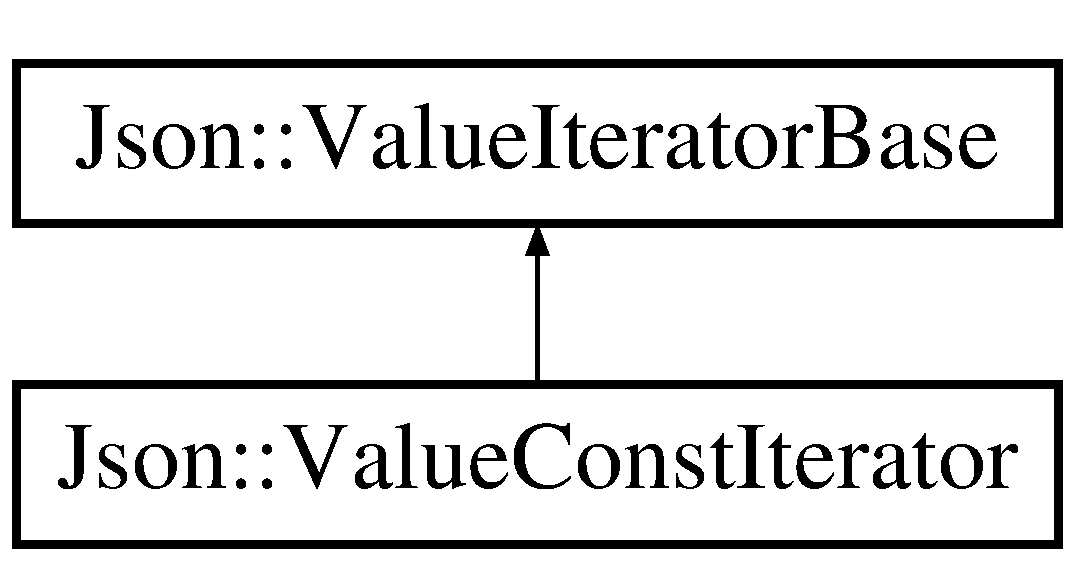
\includegraphics[height=2.000000cm]{class_json_1_1_value_const_iterator}
\end{center}
\end{figure}
\subsection*{Public Types}
\begin{DoxyCompactItemize}
\item 
\hypertarget{class_json_1_1_value_const_iterator_aa5f1707dcef4bfe73e23ddc14dbe760d}{}typedef const \hyperlink{class_json_1_1_value}{Value} {\bfseries value\+\_\+type}\label{class_json_1_1_value_const_iterator_aa5f1707dcef4bfe73e23ddc14dbe760d}

\item 
\hypertarget{class_json_1_1_value_const_iterator_aa9b05c6a37cd352ea1ee6e13b816f709}{}typedef const \hyperlink{class_json_1_1_value}{Value} \& {\bfseries reference}\label{class_json_1_1_value_const_iterator_aa9b05c6a37cd352ea1ee6e13b816f709}

\item 
\hypertarget{class_json_1_1_value_const_iterator_a400136bd8bc09e9fddec0785fa2cff14}{}typedef const \hyperlink{class_json_1_1_value}{Value} $\ast$ {\bfseries pointer}\label{class_json_1_1_value_const_iterator_a400136bd8bc09e9fddec0785fa2cff14}

\item 
\hypertarget{class_json_1_1_value_const_iterator_a0c2e33e7eb5a80dd8709fb28ece83933}{}typedef \hyperlink{class_json_1_1_value_const_iterator}{Value\+Const\+Iterator} {\bfseries Self\+Type}\label{class_json_1_1_value_const_iterator_a0c2e33e7eb5a80dd8709fb28ece83933}

\end{DoxyCompactItemize}
\subsection*{Public Member Functions}
\begin{DoxyCompactItemize}
\item 
\hypertarget{class_json_1_1_value_const_iterator_a7ef3df204a9ae83a0d8a3cd128e05c70}{}{\bfseries Value\+Const\+Iterator} (\hyperlink{class_json_1_1_value_iterator}{Value\+Iterator} const \&other)\label{class_json_1_1_value_const_iterator_a7ef3df204a9ae83a0d8a3cd128e05c70}

\item 
\hypertarget{class_json_1_1_value_const_iterator_ad1b1c11f8d7fb22d4d3c231915f2b15b}{}\hyperlink{class_json_1_1_value_iterator_base}{Self\+Type} \& {\bfseries operator=} (const \hyperlink{class_json_1_1_value_iterator_base}{Value\+Iterator\+Base} \&other)\label{class_json_1_1_value_const_iterator_ad1b1c11f8d7fb22d4d3c231915f2b15b}

\item 
\hypertarget{class_json_1_1_value_const_iterator_ab3f0c2edbfc8f7d60645f3d597d05e28}{}\hyperlink{class_json_1_1_value_iterator_base}{Self\+Type} {\bfseries operator++} (int)\label{class_json_1_1_value_const_iterator_ab3f0c2edbfc8f7d60645f3d597d05e28}

\item 
\hypertarget{class_json_1_1_value_const_iterator_a94935961e9331c6f7b907b05ec8df75e}{}\hyperlink{class_json_1_1_value_iterator_base}{Self\+Type} {\bfseries operator-\/-\/} (int)\label{class_json_1_1_value_const_iterator_a94935961e9331c6f7b907b05ec8df75e}

\item 
\hypertarget{class_json_1_1_value_const_iterator_a31415e44e44e56fb2bfda7e8bb784646}{}\hyperlink{class_json_1_1_value_iterator_base}{Self\+Type} \& {\bfseries operator-\/-\/} ()\label{class_json_1_1_value_const_iterator_a31415e44e44e56fb2bfda7e8bb784646}

\item 
\hypertarget{class_json_1_1_value_const_iterator_a2cfe2f7a94a688186efdafb1b181c319}{}\hyperlink{class_json_1_1_value_iterator_base}{Self\+Type} \& {\bfseries operator++} ()\label{class_json_1_1_value_const_iterator_a2cfe2f7a94a688186efdafb1b181c319}

\item 
\hypertarget{class_json_1_1_value_const_iterator_aeb44153d71c61ac9397a84d5ecc244c5}{}\hyperlink{class_json_1_1_value}{reference} {\bfseries operator$\ast$} () const \label{class_json_1_1_value_const_iterator_aeb44153d71c61ac9397a84d5ecc244c5}

\item 
\hypertarget{class_json_1_1_value_const_iterator_ac493d31c8eede8af10b71415fe8e624b}{}\hyperlink{class_json_1_1_value}{pointer} {\bfseries operator-\/$>$} () const \label{class_json_1_1_value_const_iterator_ac493d31c8eede8af10b71415fe8e624b}

\end{DoxyCompactItemize}
\subsection*{Private Member Functions}
\begin{DoxyCompactItemize}
\item 
\hypertarget{class_json_1_1_value_const_iterator_aa0a87edf5f1097f91dca5f2a389c4abd}{}{\bfseries Value\+Const\+Iterator} (const Value\+::\+Object\+Values\+::iterator \&current)\label{class_json_1_1_value_const_iterator_aa0a87edf5f1097f91dca5f2a389c4abd}

\end{DoxyCompactItemize}
\subsection*{Friends}
\begin{DoxyCompactItemize}
\item 
\hypertarget{class_json_1_1_value_const_iterator_aeceedf6e1a7d48a588516ce2b1983d6f}{}class {\bfseries Value}\label{class_json_1_1_value_const_iterator_aeceedf6e1a7d48a588516ce2b1983d6f}

\end{DoxyCompactItemize}
\subsection*{Additional Inherited Members}


\subsection{Detailed Description}
const iterator for object and array value. 



The documentation for this class was generated from the following files\+:\begin{DoxyCompactItemize}
\item 
C\+:/\+Users/\+Mook T/\+Desktop/item/json.\+h\item 
C\+:/\+Users/\+Mook T/\+Desktop/item/jsoncpp.\+cpp\end{DoxyCompactItemize}

\hypertarget{union_json_1_1_value_1_1_value_holder}{}\section{Json\+:\+:Value\+:\+:Value\+Holder Union Reference}
\label{union_json_1_1_value_1_1_value_holder}\index{Json\+::\+Value\+::\+Value\+Holder@{Json\+::\+Value\+::\+Value\+Holder}}
\subsection*{Public Attributes}
\begin{DoxyCompactItemize}
\item 
\hypertarget{union_json_1_1_value_1_1_value_holder_adbfb384301298844ed955ba5cf6015a0}{}Largest\+Int {\bfseries int\+\_\+}\label{union_json_1_1_value_1_1_value_holder_adbfb384301298844ed955ba5cf6015a0}

\item 
\hypertarget{union_json_1_1_value_1_1_value_holder_aab65665dc15a24a29a8e93cdeeaa7e50}{}Largest\+U\+Int {\bfseries uint\+\_\+}\label{union_json_1_1_value_1_1_value_holder_aab65665dc15a24a29a8e93cdeeaa7e50}

\item 
\hypertarget{union_json_1_1_value_1_1_value_holder_af0c5ca724e5fe3a15db773d750e2351e}{}double {\bfseries real\+\_\+}\label{union_json_1_1_value_1_1_value_holder_af0c5ca724e5fe3a15db773d750e2351e}

\item 
\hypertarget{union_json_1_1_value_1_1_value_holder_a92edab1861dadbfefd8be5fd4285eefe}{}bool {\bfseries bool\+\_\+}\label{union_json_1_1_value_1_1_value_holder_a92edab1861dadbfefd8be5fd4285eefe}

\item 
\hypertarget{union_json_1_1_value_1_1_value_holder_a70ac2b153bc405527baa3850d2ddc3cb}{}char $\ast$ {\bfseries string\+\_\+}\label{union_json_1_1_value_1_1_value_holder_a70ac2b153bc405527baa3850d2ddc3cb}

\item 
\hypertarget{union_json_1_1_value_1_1_value_holder_a1e7a5b86d4f52234f55c847ad1ce389a}{}Object\+Values $\ast$ {\bfseries map\+\_\+}\label{union_json_1_1_value_1_1_value_holder_a1e7a5b86d4f52234f55c847ad1ce389a}

\end{DoxyCompactItemize}


The documentation for this union was generated from the following file\+:\begin{DoxyCompactItemize}
\item 
C\+:/\+Users/\+Mook T/\+Desktop/item/json.\+h\end{DoxyCompactItemize}

\hypertarget{class_json_1_1_value_iterator}{}\section{Json\+:\+:Value\+Iterator Class Reference}
\label{class_json_1_1_value_iterator}\index{Json\+::\+Value\+Iterator@{Json\+::\+Value\+Iterator}}


Iterator for object and array value.  




{\ttfamily \#include $<$json.\+h$>$}

Inheritance diagram for Json\+:\+:Value\+Iterator\+:\begin{figure}[H]
\begin{center}
\leavevmode
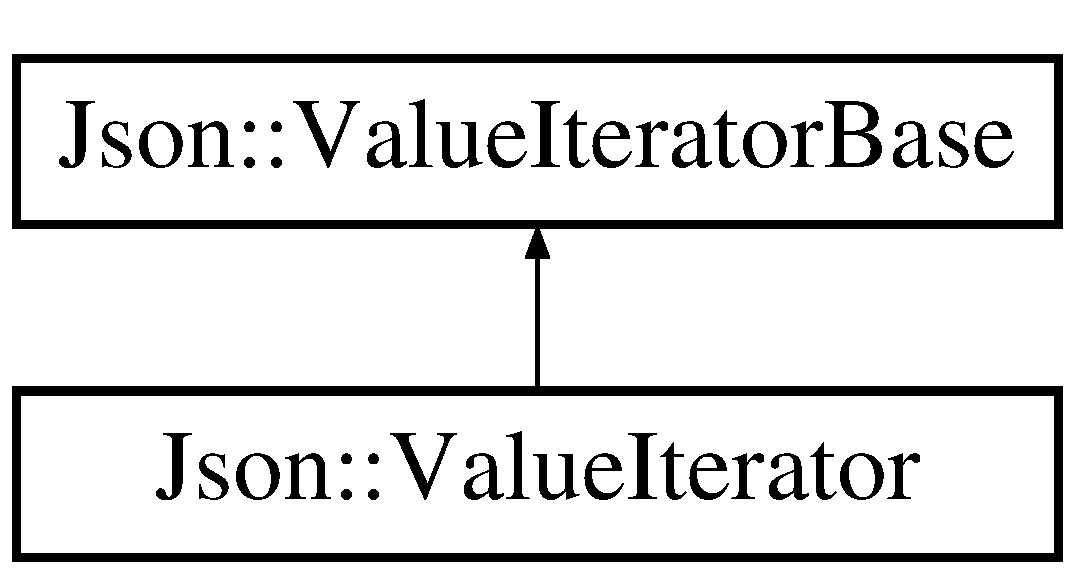
\includegraphics[height=2.000000cm]{class_json_1_1_value_iterator}
\end{center}
\end{figure}
\subsection*{Public Types}
\begin{DoxyCompactItemize}
\item 
\hypertarget{class_json_1_1_value_iterator_a2c5ba7be611f05546530c8a88b2d2e37}{}typedef \hyperlink{class_json_1_1_value}{Value} {\bfseries value\+\_\+type}\label{class_json_1_1_value_iterator_a2c5ba7be611f05546530c8a88b2d2e37}

\item 
\hypertarget{class_json_1_1_value_iterator_a308b8932ffc83eaa9d12dadd5c11a7dd}{}typedef unsigned int {\bfseries size\+\_\+t}\label{class_json_1_1_value_iterator_a308b8932ffc83eaa9d12dadd5c11a7dd}

\item 
\hypertarget{class_json_1_1_value_iterator_a2be1a9aa60bbfc8812e9dd1a7f1a8786}{}typedef int {\bfseries difference\+\_\+type}\label{class_json_1_1_value_iterator_a2be1a9aa60bbfc8812e9dd1a7f1a8786}

\item 
\hypertarget{class_json_1_1_value_iterator_ae87929b4567aa00372cf602c43b57160}{}typedef \hyperlink{class_json_1_1_value}{Value} \& {\bfseries reference}\label{class_json_1_1_value_iterator_ae87929b4567aa00372cf602c43b57160}

\item 
\hypertarget{class_json_1_1_value_iterator_acec45feb1ef1f3bf81240157d06d5432}{}typedef \hyperlink{class_json_1_1_value}{Value} $\ast$ {\bfseries pointer}\label{class_json_1_1_value_iterator_acec45feb1ef1f3bf81240157d06d5432}

\item 
\hypertarget{class_json_1_1_value_iterator_a23357670fdad61792670d86f62db7e16}{}typedef \hyperlink{class_json_1_1_value_iterator}{Value\+Iterator} {\bfseries Self\+Type}\label{class_json_1_1_value_iterator_a23357670fdad61792670d86f62db7e16}

\end{DoxyCompactItemize}
\subsection*{Public Member Functions}
\begin{DoxyCompactItemize}
\item 
\hypertarget{class_json_1_1_value_iterator_aa85aa208670891670392259efa0143bb}{}{\bfseries Value\+Iterator} (const \hyperlink{class_json_1_1_value_const_iterator}{Value\+Const\+Iterator} \&other)\label{class_json_1_1_value_iterator_aa85aa208670891670392259efa0143bb}

\item 
\hypertarget{class_json_1_1_value_iterator_a7d5e58a9a4a553968acdf3064b39d21c}{}{\bfseries Value\+Iterator} (const \hyperlink{class_json_1_1_value_iterator}{Value\+Iterator} \&other)\label{class_json_1_1_value_iterator_a7d5e58a9a4a553968acdf3064b39d21c}

\item 
\hypertarget{class_json_1_1_value_iterator_a8e23312b1db874f7e403fd7e76611bdc}{}\hyperlink{class_json_1_1_value_iterator_base}{Self\+Type} \& {\bfseries operator=} (const \hyperlink{class_json_1_1_value_iterator_base}{Self\+Type} \&other)\label{class_json_1_1_value_iterator_a8e23312b1db874f7e403fd7e76611bdc}

\item 
\hypertarget{class_json_1_1_value_iterator_abcf4ddd994a010742cd4a436d65acd08}{}\hyperlink{class_json_1_1_value_iterator_base}{Self\+Type} {\bfseries operator++} (int)\label{class_json_1_1_value_iterator_abcf4ddd994a010742cd4a436d65acd08}

\item 
\hypertarget{class_json_1_1_value_iterator_a06d6a29d96caf6af324a53973159e12b}{}\hyperlink{class_json_1_1_value_iterator_base}{Self\+Type} {\bfseries operator-\/-\/} (int)\label{class_json_1_1_value_iterator_a06d6a29d96caf6af324a53973159e12b}

\item 
\hypertarget{class_json_1_1_value_iterator_a811302a868518a0995a9def955df5720}{}\hyperlink{class_json_1_1_value_iterator_base}{Self\+Type} \& {\bfseries operator-\/-\/} ()\label{class_json_1_1_value_iterator_a811302a868518a0995a9def955df5720}

\item 
\hypertarget{class_json_1_1_value_iterator_a92146c46f8249e2b2d12869e70cd4cee}{}\hyperlink{class_json_1_1_value_iterator_base}{Self\+Type} \& {\bfseries operator++} ()\label{class_json_1_1_value_iterator_a92146c46f8249e2b2d12869e70cd4cee}

\item 
\hypertarget{class_json_1_1_value_iterator_aaa5be3457eedf0526a03b8a3b4c7c0a0}{}\hyperlink{class_json_1_1_value}{reference} {\bfseries operator$\ast$} () const \label{class_json_1_1_value_iterator_aaa5be3457eedf0526a03b8a3b4c7c0a0}

\item 
\hypertarget{class_json_1_1_value_iterator_ad9882e4ce815cef6a504afa113544bfb}{}\hyperlink{class_json_1_1_value}{pointer} {\bfseries operator-\/$>$} () const \label{class_json_1_1_value_iterator_ad9882e4ce815cef6a504afa113544bfb}

\end{DoxyCompactItemize}
\subsection*{Private Member Functions}
\begin{DoxyCompactItemize}
\item 
\hypertarget{class_json_1_1_value_iterator_afb06ea21add440c78c27dc49570460a5}{}{\bfseries Value\+Iterator} (const Value\+::\+Object\+Values\+::iterator \&current)\label{class_json_1_1_value_iterator_afb06ea21add440c78c27dc49570460a5}

\end{DoxyCompactItemize}
\subsection*{Friends}
\begin{DoxyCompactItemize}
\item 
\hypertarget{class_json_1_1_value_iterator_aeceedf6e1a7d48a588516ce2b1983d6f}{}class {\bfseries Value}\label{class_json_1_1_value_iterator_aeceedf6e1a7d48a588516ce2b1983d6f}

\end{DoxyCompactItemize}
\subsection*{Additional Inherited Members}


\subsection{Detailed Description}
Iterator for object and array value. 

The documentation for this class was generated from the following files\+:\begin{DoxyCompactItemize}
\item 
C\+:/\+Users/\+Mook T/\+Desktop/item/json.\+h\item 
C\+:/\+Users/\+Mook T/\+Desktop/item/jsoncpp.\+cpp\end{DoxyCompactItemize}

\hypertarget{class_json_1_1_value_iterator_base}{}\section{Json\+:\+:Value\+Iterator\+Base Class Reference}
\label{class_json_1_1_value_iterator_base}\index{Json\+::\+Value\+Iterator\+Base@{Json\+::\+Value\+Iterator\+Base}}


base class for \hyperlink{class_json_1_1_value}{Value} iterators.  




{\ttfamily \#include $<$json.\+h$>$}

Inheritance diagram for Json\+:\+:Value\+Iterator\+Base\+:\begin{figure}[H]
\begin{center}
\leavevmode
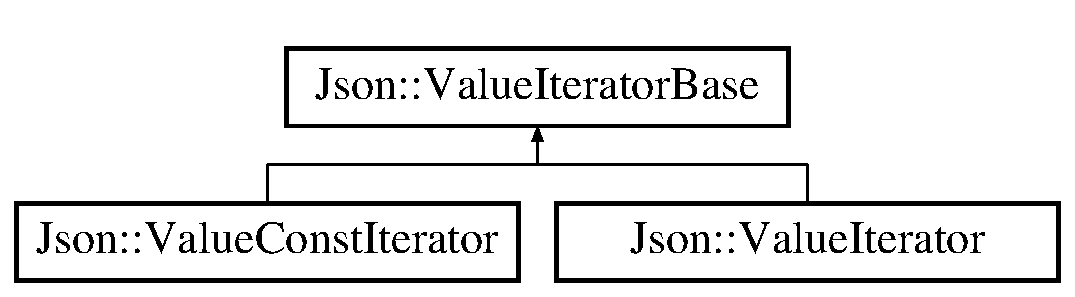
\includegraphics[height=2.000000cm]{class_json_1_1_value_iterator_base}
\end{center}
\end{figure}
\subsection*{Public Types}
\begin{DoxyCompactItemize}
\item 
\hypertarget{class_json_1_1_value_iterator_base_a02fd11a4fbdc0007da1e8bcf5e6b83c3}{}typedef std\+::bidirectional\+\_\+iterator\+\_\+tag {\bfseries iterator\+\_\+category}\label{class_json_1_1_value_iterator_base_a02fd11a4fbdc0007da1e8bcf5e6b83c3}

\item 
\hypertarget{class_json_1_1_value_iterator_base_a9d3a3c7ce5cdefe23cb486239cf07bb5}{}typedef unsigned int {\bfseries size\+\_\+t}\label{class_json_1_1_value_iterator_base_a9d3a3c7ce5cdefe23cb486239cf07bb5}

\item 
\hypertarget{class_json_1_1_value_iterator_base_a4e44bf8cbd17ec8d6e2c185904a15ebd}{}typedef int {\bfseries difference\+\_\+type}\label{class_json_1_1_value_iterator_base_a4e44bf8cbd17ec8d6e2c185904a15ebd}

\item 
\hypertarget{class_json_1_1_value_iterator_base_a9d2a940d03ea06d20d972f41a89149ee}{}typedef \hyperlink{class_json_1_1_value_iterator_base}{Value\+Iterator\+Base} {\bfseries Self\+Type}\label{class_json_1_1_value_iterator_base_a9d2a940d03ea06d20d972f41a89149ee}

\end{DoxyCompactItemize}
\subsection*{Public Member Functions}
\begin{DoxyCompactItemize}
\item 
\hypertarget{class_json_1_1_value_iterator_base_afc656672ac28502f640ade32c38c1b56}{}bool {\bfseries operator==} (const \hyperlink{class_json_1_1_value_iterator_base}{Self\+Type} \&other) const \label{class_json_1_1_value_iterator_base_afc656672ac28502f640ade32c38c1b56}

\item 
\hypertarget{class_json_1_1_value_iterator_base_a18c2dd42e0bb989ace141bfe9de52792}{}bool {\bfseries operator!=} (const \hyperlink{class_json_1_1_value_iterator_base}{Self\+Type} \&other) const \label{class_json_1_1_value_iterator_base_a18c2dd42e0bb989ace141bfe9de52792}

\item 
\hypertarget{class_json_1_1_value_iterator_base_ab786787fcad68ca5e8745aaf520fa17f}{}difference\+\_\+type {\bfseries operator-\/} (const \hyperlink{class_json_1_1_value_iterator_base}{Self\+Type} \&other) const \label{class_json_1_1_value_iterator_base_ab786787fcad68ca5e8745aaf520fa17f}

\item 
\hyperlink{class_json_1_1_value}{Value} \hyperlink{class_json_1_1_value_iterator_base_aa2ff5e79fc96acd4c3cd288e92614fc7}{key} () const 
\item 
\hypertarget{class_json_1_1_value_iterator_base_aa90591f5f7f8d2f06cc4605816b53738}{}U\+Int \hyperlink{class_json_1_1_value_iterator_base_aa90591f5f7f8d2f06cc4605816b53738}{index} () const \label{class_json_1_1_value_iterator_base_aa90591f5f7f8d2f06cc4605816b53738}

\begin{DoxyCompactList}\small\item\em Return the index of the referenced \hyperlink{class_json_1_1_value}{Value}, or -\/1 if it is not an array\+Value. \end{DoxyCompactList}\item 
std\+::string \hyperlink{class_json_1_1_value_iterator_base_a46a67081a5ef8d83f25ec15035403ce0}{name} () const 
\item 
char const $\ast$ \hyperlink{class_json_1_1_value_iterator_base_ac3aa3870761342e47c6486d81f643c6c}{member\+Name} () const 
\item 
char const $\ast$ \hyperlink{class_json_1_1_value_iterator_base_a543d4e73e3d2d121bc287b24231386c3}{member\+Name} (char const $\ast$$\ast$end) const 
\item 
\hypertarget{class_json_1_1_value_iterator_base_a640e990e5f03a96fd650122a2906f59d}{}{\bfseries Value\+Iterator\+Base} (const Value\+::\+Object\+Values\+::iterator \&current)\label{class_json_1_1_value_iterator_base_a640e990e5f03a96fd650122a2906f59d}

\end{DoxyCompactItemize}
\subsection*{Protected Member Functions}
\begin{DoxyCompactItemize}
\item 
\hypertarget{class_json_1_1_value_iterator_base_a40a20c65abc423a26e3aae68d9a0525c}{}\hyperlink{class_json_1_1_value}{Value} \& {\bfseries deref} () const \label{class_json_1_1_value_iterator_base_a40a20c65abc423a26e3aae68d9a0525c}

\item 
\hypertarget{class_json_1_1_value_iterator_base_afe58f9534e1fd2033419fd9fe244551e}{}void {\bfseries increment} ()\label{class_json_1_1_value_iterator_base_afe58f9534e1fd2033419fd9fe244551e}

\item 
\hypertarget{class_json_1_1_value_iterator_base_affc8cf5ff54a9f432cc693362c153fa6}{}void {\bfseries decrement} ()\label{class_json_1_1_value_iterator_base_affc8cf5ff54a9f432cc693362c153fa6}

\item 
\hypertarget{class_json_1_1_value_iterator_base_ad6c553b249e89e3dc9933e100ccbe064}{}difference\+\_\+type {\bfseries compute\+Distance} (const \hyperlink{class_json_1_1_value_iterator_base}{Self\+Type} \&other) const \label{class_json_1_1_value_iterator_base_ad6c553b249e89e3dc9933e100ccbe064}

\item 
\hypertarget{class_json_1_1_value_iterator_base_a21820d6ee564e541bd118b21e4741962}{}bool {\bfseries is\+Equal} (const \hyperlink{class_json_1_1_value_iterator_base}{Self\+Type} \&other) const \label{class_json_1_1_value_iterator_base_a21820d6ee564e541bd118b21e4741962}

\item 
\hypertarget{class_json_1_1_value_iterator_base_a496e6aba44808433ec5858c178be5719}{}void {\bfseries copy} (const \hyperlink{class_json_1_1_value_iterator_base}{Self\+Type} \&other)\label{class_json_1_1_value_iterator_base_a496e6aba44808433ec5858c178be5719}

\end{DoxyCompactItemize}
\subsection*{Private Attributes}
\begin{DoxyCompactItemize}
\item 
\hypertarget{class_json_1_1_value_iterator_base_ab3138ce8af8301cca3b041ea55cb922a}{}Value\+::\+Object\+Values\+::iterator {\bfseries current\+\_\+}\label{class_json_1_1_value_iterator_base_ab3138ce8af8301cca3b041ea55cb922a}

\item 
\hypertarget{class_json_1_1_value_iterator_base_a3e08b114a1aed9bde518c527f94a8c59}{}bool {\bfseries is\+Null\+\_\+}\label{class_json_1_1_value_iterator_base_a3e08b114a1aed9bde518c527f94a8c59}

\end{DoxyCompactItemize}


\subsection{Detailed Description}
base class for \hyperlink{class_json_1_1_value}{Value} iterators. 



\subsection{Member Function Documentation}
\hypertarget{class_json_1_1_value_iterator_base_aa2ff5e79fc96acd4c3cd288e92614fc7}{}\index{Json\+::\+Value\+Iterator\+Base@{Json\+::\+Value\+Iterator\+Base}!key@{key}}
\index{key@{key}!Json\+::\+Value\+Iterator\+Base@{Json\+::\+Value\+Iterator\+Base}}
\subsubsection[{key() const }]{\setlength{\rightskip}{0pt plus 5cm}{\bf Value} Json\+::\+Value\+Iterator\+Base\+::key (
\begin{DoxyParamCaption}
{}
\end{DoxyParamCaption}
) const}\label{class_json_1_1_value_iterator_base_aa2ff5e79fc96acd4c3cd288e92614fc7}
Return either the index or the member name of the referenced value as a \hyperlink{class_json_1_1_value}{Value}. \hypertarget{class_json_1_1_value_iterator_base_ac3aa3870761342e47c6486d81f643c6c}{}\index{Json\+::\+Value\+Iterator\+Base@{Json\+::\+Value\+Iterator\+Base}!member\+Name@{member\+Name}}
\index{member\+Name@{member\+Name}!Json\+::\+Value\+Iterator\+Base@{Json\+::\+Value\+Iterator\+Base}}
\subsubsection[{member\+Name() const }]{\setlength{\rightskip}{0pt plus 5cm}char const $\ast$ Json\+::\+Value\+Iterator\+Base\+::member\+Name (
\begin{DoxyParamCaption}
{}
\end{DoxyParamCaption}
) const}\label{class_json_1_1_value_iterator_base_ac3aa3870761342e47c6486d81f643c6c}
Return the member name of the referenced \hyperlink{class_json_1_1_value}{Value}. \char`\"{}\char`\"{} if it is not an object\+Value. \begin{DoxyRefDesc}{Deprecated}
\item[\hyperlink{deprecated__deprecated000004}{Deprecated}]This cannot be used for U\+T\+F-\/8 strings, since there can be embedded nulls. \end{DoxyRefDesc}
\hypertarget{class_json_1_1_value_iterator_base_a543d4e73e3d2d121bc287b24231386c3}{}\index{Json\+::\+Value\+Iterator\+Base@{Json\+::\+Value\+Iterator\+Base}!member\+Name@{member\+Name}}
\index{member\+Name@{member\+Name}!Json\+::\+Value\+Iterator\+Base@{Json\+::\+Value\+Iterator\+Base}}
\subsubsection[{member\+Name(char const $\ast$$\ast$end) const }]{\setlength{\rightskip}{0pt plus 5cm}char const $\ast$ Json\+::\+Value\+Iterator\+Base\+::member\+Name (
\begin{DoxyParamCaption}
\item[{char const $\ast$$\ast$}]{end}
\end{DoxyParamCaption}
) const}\label{class_json_1_1_value_iterator_base_a543d4e73e3d2d121bc287b24231386c3}
Return the member name of the referenced \hyperlink{class_json_1_1_value}{Value}, or N\+U\+L\+L if it is not an object\+Value. \begin{DoxyNote}{Note}
Better version than \hyperlink{class_json_1_1_value_iterator_base_ac3aa3870761342e47c6486d81f643c6c}{member\+Name()}. Allows embedded nulls. 
\end{DoxyNote}
\hypertarget{class_json_1_1_value_iterator_base_a46a67081a5ef8d83f25ec15035403ce0}{}\index{Json\+::\+Value\+Iterator\+Base@{Json\+::\+Value\+Iterator\+Base}!name@{name}}
\index{name@{name}!Json\+::\+Value\+Iterator\+Base@{Json\+::\+Value\+Iterator\+Base}}
\subsubsection[{name() const }]{\setlength{\rightskip}{0pt plus 5cm}std\+::string Json\+::\+Value\+Iterator\+Base\+::name (
\begin{DoxyParamCaption}
{}
\end{DoxyParamCaption}
) const}\label{class_json_1_1_value_iterator_base_a46a67081a5ef8d83f25ec15035403ce0}
Return the member name of the referenced \hyperlink{class_json_1_1_value}{Value}, or \char`\"{}\char`\"{} if it is not an object\+Value. \begin{DoxyNote}{Note}
Avoid {\ttfamily c\+\_\+str()} on result, as embedded zeroes are possible. 
\end{DoxyNote}


The documentation for this class was generated from the following files\+:\begin{DoxyCompactItemize}
\item 
C\+:/\+Users/\+Mook T/\+Desktop/item/json.\+h\item 
C\+:/\+Users/\+Mook T/\+Desktop/item/jsoncpp.\+cpp\end{DoxyCompactItemize}

\hypertarget{class_json_1_1_writer}{}\section{Json\+:\+:Writer Class Reference}
\label{class_json_1_1_writer}\index{Json\+::\+Writer@{Json\+::\+Writer}}


Abstract class for writers.  




{\ttfamily \#include $<$json.\+h$>$}

Inheritance diagram for Json\+:\+:Writer\+:\begin{figure}[H]
\begin{center}
\leavevmode
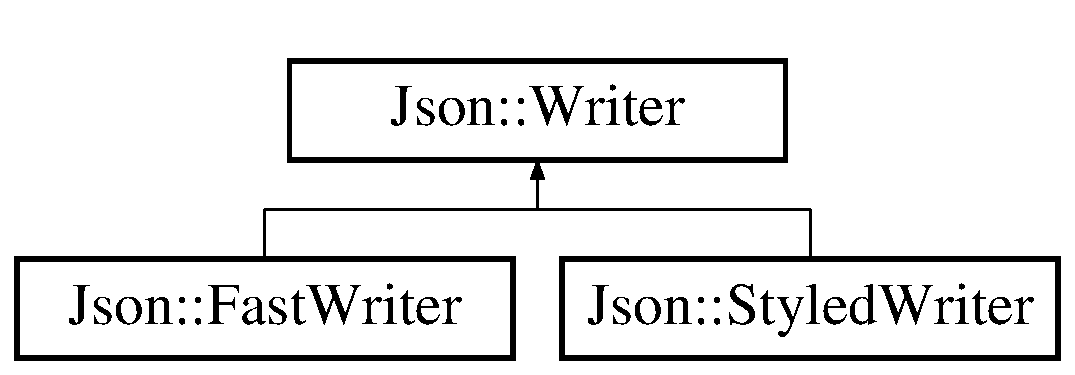
\includegraphics[height=2.000000cm]{class_json_1_1_writer}
\end{center}
\end{figure}
\subsection*{Public Member Functions}
\begin{DoxyCompactItemize}
\item 
\hypertarget{class_json_1_1_writer_a7b2273a4ffd6f32b369ac8a53b7b5a0d}{}virtual std\+::string {\bfseries write} (const \hyperlink{class_json_1_1_value}{Value} \&root)=0\label{class_json_1_1_writer_a7b2273a4ffd6f32b369ac8a53b7b5a0d}

\end{DoxyCompactItemize}


\subsection{Detailed Description}
Abstract class for writers. 

\begin{DoxyRefDesc}{Deprecated}
\item[\hyperlink{deprecated__deprecated000007}{Deprecated}]Use \hyperlink{class_json_1_1_stream_writer}{Stream\+Writer}. (And really, this is an implementation detail.) \end{DoxyRefDesc}


The documentation for this class was generated from the following files\+:\begin{DoxyCompactItemize}
\item 
C\+:/\+Users/\+Mook T/\+Desktop/item/json.\+h\item 
C\+:/\+Users/\+Mook T/\+Desktop/item/jsoncpp.\+cpp\end{DoxyCompactItemize}

%--- End generated contents ---

% Index
\backmatter
\newpage
\phantomsection
\clearemptydoublepage
\addcontentsline{toc}{chapter}{Index}
\printindex

\end{document}
